\documentclass[a4paper,10pt]{book}
\usepackage[english]{babel}
\usepackage[T1]{fontenc}
\usepackage[latin1]{inputenc}
\usepackage{float}
\usepackage[center]{subfigure}
%\usepackage[light, first]{draftcopy}
\usepackage{fancyhdr}
\usepackage{tabularx}
\usepackage{booktabs}
\usepackage{amsmath}
\usepackage{amssymb}
%\usepackage{footnpag}
\usepackage[perpage,symbol*]{footmisc}
\usepackage[square,comma,sort&compress,numbers]{natbib}
\usepackage{bibentry}
%\usepackage[small,hang,bf]{caption2}
\usepackage[small,bf]{caption2}
%\usepackage{multicol}
%\usepackage{times}
%\usepackage{index}
%\usepackage{theorem}
%\usepackage{tabls}
%\usepackage{wrapfig}
\usepackage{a4wide}
\usepackage{PhD}
\usepackage{ifthen}
\usepackage{mystuff}
%\usepackage{hyperref}
\usepackage[pdftex,colorlinks=true,
				 pdfstartview=FitV,
				 linkcolor=blue,
				 citecolor=blue,
				 urlcolor=blue,
		  ]{hyperref}
%          \pdfinfo{
%            /Title      (Why the system crashed)
%            /Author     (Jonas Juselius)
%            /Keywords   (XML Java OOA/OOD Corba COM)
%          }
\newif\ifappendix
\ifpdf
  \appendixtrue
%  \appendixfalse
%  \usepackage[dvips]{graphicx}
  \usepackage{pdfpages}
  \pdfcompresslevel=1
\else
%  \appendixfalse
  \appendixtrue
  \usepackage[dvips]{graphicx}
\fi

\newcommand\Eq[1]{Eq.~\ref{#1}}
\newcommand\Fig[1]{Fig.~\ref{#1}}
\newcommand\Ch[1]{Chap.~\ref{#1}}
\newcommand\Sec[1]{Sec.~\ref{#1}}


%\graphicspath{{../calc/}}
%\shortindexingon
%\makeindex
%\shortindexingon
%\makeindex

%\numberwithin{equation}{chapter}
%\bibpunct{[}{]}{,}{n}{}{}
%\setlength{\bibsep}{0pt}

\bibliographystyle{PhD2}
\nobibliography*
\defcitealias{Juselius:t99}{Article~I}
\defcitealias{Juselius:t00}{Article~II}
\defcitealias{Juselius:t00a}{Article~III}
\defcitealias{Juselius:t01}{Article~IV}
\defcitealias{Juselius:t01a}{Article~V}
\defcitealias{Juselius:t03}{Article~VI}
\defcitealias{Juselius:t04}{Article~VII}
\defcitealias{Juselius:t04c}{Article~VIII}

\begin{document}
\pagestyle{fancy}
\fancyfoot{}
\fancyhead{}

%\floatstyle{topruled}
%\restylefloat{table}
%\restylefloat{figure}

\renewcommand{\chaptermark}[1]{\markboth{\sf\thechapter.\ #1}{}}
\renewcommand{\sectionmark}[1]{\markboth{\sf\thesection.\ #1}{}}
\renewcommand{\subsectionmark}[1]{}

\fancyhead[RE,LO]{{\rmfamily\thepage}}

\title{Theoretical investigation of magnetically induced \\currents in 
closed-shell molecules}

\subtitle{Dissertation for the degree of Doctor Philosophiae}
\author{{\sf Jonas Jus\'elius}}
\address{
{\sf University of Helsinki}\\
{\sf Department of Chemistry}\\
{\sf Laboratory for Instruction in Swedish}\\
{\sf P.O. Box 55 (A.I. Virtasen Aukio 1) }\\
{\sf FIN-00014 University of Helsinki, Finland}
}
\years{2004}
\abstract{To be presented, with the assent of the Faculty
of Science, University of Helsinki, for public discussion in Auditorium A129,
Department of Chemistry (A.I. Virtasen Aukio 1, Helsinki), 
December the 20th, 2004, at noon.\\[3mm]
\centerline{\sf Helsinki 2004}}

\maketitle
\newpage\thispagestyle{empty}
\vspace*{5cm}
\sf\noindent
{\large Supervised by}\\[2mm]
{\large Dr. Dage Sundholm\\
Department of Chemistry\\
University of Helsinki}\\[2cm]
{\large Reviewed by}\\[2mm]
{\large Prof. Kenneth Ruud\\
Department of Chemistry\\
University of Troms\o}\\[0.5cm]
{\large Dr. Juha Vaara\\
Department of Chemistry\\
University of Helsinki}\\[1cm]
\vfill
{\large\noindent
ISBN 952-91-8135-3 (paperback)\\[1mm]
ISBN 952-10-2247-7 (PDF)\\[1mm]
http://ethesis.helsinki.fi\\[3mm]
Yliopistopaino\\
Helsinki 2004
}
\rm

\chapter*{Abstract}
\pagenumbering{roman}
\thispagestyle{empty}
\addcontentsline{toc}{chapter}{Abstract}
%\setcounter{page}{1}
%\newpage\thispagestyle{empty}
%\vspace*{2.2cm}
%{\bf\Huge Abstract}
%\vspace{1cm}

The work presented in this thesis is concerned with the theory and development
of methods for {\em ab initio} calculation of  magnetically induced current
densities in closed-shell molecules. Two new methods are presented.  The
underlying theory of both methods is closely related to the theory of nuclear
magnetic shielding (NMR) calculations.
The Aromatic Ring-Current Shieldings (ARCS) method can be viewed
as an experimental procedure in a theoretical framework. In the ARCS method, 
the strength of the magnetically induced ring current in aromatic molecules is
extracted from the long-range part of the calculated NMR shielding function
through a fitting procedure.

In the Gauge-Including Magnetically Induced Currents (GIMIC) method, the
magnetically induced current density in molecules is calculated explicitly. In
order to overcome problems with the dependence on the magnetic gauge origin,
Gauge-Including Atomic Orbitals (GIAOs) are employed. The advantage of the
GIMIC method is high accuracy, and the applicability to mean-field,
density-functional and electron-correlated levels of theory. The GIMIC method
is fast and can be applied to large closed-shell molecules of
nano-technological importance. The method can also reveal the detailed
structure of the current density in molecules.  Using quadrature, the
GIMIC method can be used to obtain the strength of induced currents in
aromatic molecules.

The ARCS and GIMIC methods have been applied to a variety of
different molecular systems, both to test their applicability and accuracy,
and in an attempt to understand and classify molecular aromaticity.
\newpage
\thispagestyle{plain}
\vspace*{2.0cm}
{\noindent\bf\Huge List of publications}
\addcontentsline{toc}{chapter}{List of publications}
\vspace{1cm}

\section*{List of publications included in the thesis}
\renewcommand{\theenumi}{\Roman{enumi}}
\begin{enumerate}
\item \bibentry{Juselius:t99}.
\item \bibentry{Juselius:t00}.
\item \bibentry{Juselius:t00a}.
\item \bibentry{Juselius:t01}.
\item \bibentry{Juselius:t01a}.
\item \bibentry{Juselius:t03}.
\item \bibentry{Juselius:t04}.
%\item \bibentry{Juselius:t04c}

\end{enumerate}

\section*{List of other publications}
\begin{enumerate}
\item \bibentry{Berger:t01}.
\item \bibentry{Juselius:t04e}.
\item \bibentry{Juselius:t04c}.
\item \bibentry{Juselius:t04f}.
\item \bibentry{Juselius:t04b}.
\item \bibentry{Lin:t04}.
\end{enumerate}

\renewcommand{\theenumi}{\arabic{enumi}}


\chapter*{\vspace{-2cm}Acknowledgments}
\addcontentsline{toc}{chapter}{Acknowledgments}
%\thispagestyle{empty}
%\newpage\thispagestyle{empty}\phantom,
%\newpage\thispagestyle{empty}
%\vspace*{0.5cm}
%{\bf\Huge Acknowledgments}
%\vspace{1cm}

I would like to express my deepest gratitude to my supervisor Dage Sundholm,
who is an excellent scientist, a top-notch supervisor and a good 
friend. In his good-humored way, he always seems to find time to listen and 
help. He also knows when to come and ''kick in my door'' and give me a push, 
without interfering more than needed. I thank Pekka Pyykk� for hiring me to
the group already in my second year at the university. I consider Pekka my
second supervisor, since he has spent numerous hours explaining and teaching
me both quantum mechanics and chemistry. Pekka's enormous knowledge in
physics, quantum mechanics and chemistry has been an invaluable asset during
my studies. I also jointly thank Pekka and Dage for sending me to many 
research schools and conferences over the years.

I owe a lot of gratitude to the past and present members of the Laboratory of
Instruction in Swedish: Mikael Johansson, Henrik Konschin, Olli Lehtonen,
Ying-Chan Lin, Bjarne Lindstr�m, Michael Patzschke, Stefan Taubert, Bertel
Westermark, Pekka Manninen, Michaela Ekholm, Carola Olkkonen, Nino Runeberg,
Toomas Tamm, Henrik Tylli and Juha Vaara. I thank you for what you have taught
me, for proof-reading manuscripts and all the discussions in the coffee room,
ranging from chemistry to politics. One person who deserves an extra big 
thank-you is the sunshine of the laboratory, Susanne Lundberg, who somehow
always manages to be in a cheerful mood and never fails to be helpful.

I especially want to thank J�rgen Gauss for inviting me to Mainz, and for his
great hospitality during my stays. I had a very good time in Mainz, both
scientifically and socially, not least thanks to the Mainz group at the time:
Alexander Auer, Michael Harding, Miriam Heckert, Oliver Heun, Uli H�berle,
Dan Jonsson, Mih�ly K�llay, Michael Lenhart and Thorsten Metzroth.

I also want to thank my co-authors for many fruitful collaborations: 
Raphael Berger, Rui Fausto, J�rgen Gauss, Mikael Johansson, 
Leonid Khriachtchev, Antti Lignell, Ying-Chan Lin, Ermelinda Ma\c{c}\^oas, 
Michael Patzschke, Mika Petterson, Markku R�s�nen, Elena Savchenko,
Michal Straka and  Dage Sunholm.
I thank Magnus Ehrnrooths stiftelse, Waldemar von Frenkells stiftelse, the
LASKEMO graduate school, the Academy of Finland and the University of
Helsinki for their generous support.

Last, but not least, I want to thank my family and friends. 
I thank my brothers, Mikael and Joakim Jus\'elius for just
being there. My mother Katarina Jus\'elius, and S\o ren Johansen I thank for
their enourmous support, and for the beautiful summers at Troll�n.
I also thank my father Jussi Jus\'elius, and Tuula Jus\'elius for being
supportive. My grandmother, Maija Jus\'elius deserves a huge
hug for being there for me, and for cooking wonderful dinners every Sunday. I
also thank my godmother Kaisa Lillqvist, and my Danish ''brothers'' for being
so nice.  I want to thank Tommy V�nsk� for being such a good friend, for the
rock climbing trips around Europe, for the countless hours in the pool hall,
and for the afternoons on Troll�n, sitting in the sun and contemplating
quantum mechanics.

Finally, I want to express my greatest gratitude to my love, Mia Tenhunen, for
putting up with me, and always supporting me. You have taught me so many
things that cannot be aquired by reading books. I thank you for your patience
and understanding, for being a worthy opponent, but most of all, for just
being you. I also silently thank the rest of my good friends, you know how you
are, but you are too many to fit on this page.

\vspace{0.5cm}
\begin{center}
Jonas Jus\'elius\\[5mm]
Helsinki, \today
\end{center}

%\chapter*{List of publications}
%\newpage\thispagestyle{empty}
\tableofcontents

\chapter*{List of abbreviations}
\addcontentsline{toc}{chapter}{List of abbreviations}
\begin{tabular}{ll}
\bf{AO} & Atomic Orbital \\
\bf{ARCS} & Aromatic Ring-Current Shielding \\
\bf{CC} &   Coupled-Cluster \\
\bf{CCSD} & Coupled-Cluster with Single and Double excitations \\
\bf{CHF} & Coupled Hartree--Fock \\
\bf{CI} & Configuration Interaction \\
\bf{CSGT} & Continuous Set of Gauge Transformations \\
\bf{CTOCD}& Continuous Transformation of Origin of the Current Density \\
\bf{CPHF} & Coupled Perturbed Hartree--Fock \\
\bf{DFT} & Density-Functional Theory \\
\bf{GIMIC} & Gauge-Including Magnetically Induced Current \\
\bf{GIAO} & Gauge-Including Atomic Orbital \\
\bf{GTO} & Gaussian Type Orbital \\
\bf{HF} & Hartree--Fock \\
\bf{LCAO} & Linear Combination of Atomic Orbitals \\
\bf{MBPT} & Many-Body Perturbation Theory \\
\bf{MP2} & M\o ller--Plesset perturbation theory to the second order \\
\bf{MO} & Molecular Orbital \\
\bf{NICS} & Nucleus-Independent Chemical Shift \\
\bf{NMR} & Nuclear Magnetic Resonance \\
\bf{PARCS} & Planar Aromatic Ring-Current Shielding \\
\bf{SCF} & Self-Consistent Field  \\
\end{tabular}


\chapter{Introduction}
%\pagestyle{fancy}
\fancyhead[RE,LO]{\leftmark}
\fancyhead[RO,LE]{{\rmfamily\thepage}}
\pagenumbering{arabic}
\setcounter{page}{1}
Aromaticity is an important concept in chemistry. Although widely used, the
aromaticity concept is not uniquely defined. High stability, reduced bond
length alternation, low reactivity and increased response to magnetic fields
are typical characteristics for aromatic molecules.  One of the motivations
for starting the work presented in this thesis was to try to understand the
chemical concept of aromaticity from a theoretical point of view.

For a long time, aromaticity was considered to be a property of only
cyclic, planar organic molecules having 4$n$+2 $\pi$-electrons. However, the
concept of aromaticity has later been extended to include also inorganic and
non-planar, spherical and even linear molecules! The idea that only the 
$\pi$-electrons contribute to aromaticity has been revised to include
$\sigma$-electrons. Aromaticity has previously been defined on the basis of
energetics, as well as geometric and magnetic criteria, such as nuclear
magnetic shielding tensors and magnetic susceptibilities 
\cite{Fleischer:94,Elvidge:61,Abraham:65,Schleyer:96b,Subramanian:96,Buehl:98,
Julg:67,Bird:85,Jug:91,Minkin:94,Schleyer:95a,Jiao:96,Schleyer:96a,Cernusak:97,
Zanasi:97,Cyranski:98}. The degree of aromaticity is even more difficult to
deduce from energetic and structural data than from magnetic criteria such as
elevated magnetic susceptibility, susceptibility anisotropies, and
Nucleus-Independent Chemical Shift (NICS) values \cite{Schleyer:95a}.  
With this in mind it might seem
futile to try to come up with a single theoretical model which would be able
to quantify aromaticity.

While aromaticity, like beauty, may be in the eye of the beholder, the
magnetically induced currents in a molecule are unequivocally defined.  In the
pursuit to understand and quantify aromaticity a very pragmatic view is hence
adopted here. The key molecular property for a molecule to be aromatic is the
ability to sustain a {\em net} electrical current when subjected to a magnetic
field.  A ring current does itself not guarantee aromaticity, but failure to
sustain a ring current guarantees that the molecule is not aromatic.
Throughout this thesis the word aromaticity is used as a synonym for ''ability
to sustain a ring current``, regardless of any other aromatic properties.

The calculation of time-independent ring
currents of closed-shell molecules, and the strength of the currents are
the main topic of this thesis.  Whether the strengths of these currents can
be used to classify aromatic strength can be debated. 
In order to lay the foundation for understanding the work presented in this
thesis, I will review the most important aspects of the underlying 
theoretical framework. \Ch{ch:energy} gives a short review of the Schr�dinger
equation and the most common approximations and methods for calculating
the molecular ground-state energy. In \Ch{ch:molprop} general methods for 
obtaining molecular ground-state properties are discussed, with focus on 
derivative theory. The theory of magnetic interactions, and in particular
interactions between electrons and an external magnetic field, are considered
in \Ch{ch:magnet}. \Ch{ch:magnet} also touches the subject of calculating
nuclear magnetic shielding parameters, and the problem of gauge invariance. 
Ring currents and aromaticity are discussed in some detail in \Ch{ch:current},
with examples of various kinds of aromaticity. \Ch{ch:current} also presents
the theory underlying our first quantitative method for estimating the
strength of the ring current, the Aromatic Ring-Current Shieldings (ARCS)
method \cite{Juselius:t99}. In \Ch{ch:gimic} {\em ab
initio} ring-current models are presented, with an in-depth discussion of 
the new Gauge-Including Magnetically Induced Currents (GIMIC)
method \cite{Juselius:t04}. \Ch{ch:synopsis}
provides an summary of the original scientific papers included in the
appendices.

\chapter{The molecular energy}
\label{ch:energy}
In this chapter some of the standard methods and approximations of 
quantum chemistry are reviewed. Only the theory of time-independent,
closed-shell molecules in a non-relativistic framework will be considered.

The starting point for most of quantum chemistry is the time-independent
Schr�dinger equation which can be compactly written $\hat H\Psi=E\Psi$, where
$\hat H$ is the Hamiltonian and $\Psi$ is the wave function. 
In atomic units\footnote{In atomic units $e=\hbar=m_e=4\pi\epsilon_0=1$.}
the molecular Hamiltonian in its simplest form is given by
\begin{equation}
\hat H=-\oover{2}\sum_i^N\nabla_i^2+\sum_{i>j}^N\frac{1}{r_{ij}}-
\sum_A^K\sum_i^N\frac{Z_A}{r_{Ai}}-
\sum_A^K\oover{2M_A}\nabla_A^2+\sum_{A>B}^K\frac{Z_A Z_B}{R_{AB}},
\label{hamiltonian}
\end{equation} 
where $N$ is the number of electrons, $K$ the number of nuclei, $M_K$ the
nuclear mass and $Z_A$ the nuclear charge. The operator $r_{ij}$ is the
inter-electronic distance between electrons $i$ and $j$.
Using the Born--Oppenheimer approximation \cite{Oppenheimer:27}
the nuclear degrees of freedom can be separated from the electronic degrees of
freedom, and the (time-independent) wave function then depends 
only parametrically on the nuclear coordinates. The wave function
is then dependent on $4N$ variables, including the electron spin. Already for
moderately complicated molecules, containing hundreds or thousands of
electrons, this function quickly becomes extremely complicated. 

The electronic wave function must be square integrable and normalized to be
consistent with the Born probability interpretation \cite{Gas:96}
\begin{equation} 
1=\int d\mbf x_1\ldots d\mbf x_N\Psi(\mbf x_1\ldots \mbf x_N)^*
\Psi(\mbf x_1\ldots \mbf x_N),
\end{equation} 
where $\Psi^*$ denotes the complex conjugate and 
$\mbf x=(r_1, r_2, r_3,\sigma)$, where $\sigma\in\{\alpha,\beta\}$ is the 
electron spin coordinate. In closed-shell molecules the spin can be be
integrated out, leaving three spatial degrees of freedom per electron.

In accordance with the above condition the electron density of
the system is
\begin{equation} 
\rho(\mbf{r})=N
\int d\mbf r_2 \ldots d\mbf r_{N} \Psi(\mbf r,\mbf r_2,\ldots \mbf r_N )^*
\Psi(\mbf r,\mbf r_2,\ldots \mbf r_N ).
\end{equation} 

To deal with this formidable function, one usually expands it in a basis of
$3N$-dimensional functions.  The basis functions are formed by
anti-symmetrizing direct products of $N$ one-particle functions with respect to
the particle indices. These functions can conveniently be written as Slater
determinants, $\Phi=\det|\phi_p(\mbf r_1)\ldots\phi_q(\mbf r_N)|$.  
The one-particle
functions are usually taken as linear combinations of atom-centered functions
\begin{equation}
\phi_a(\mbf r)=\sum_\mu^{N_{AO}} C_{\mu a} \chi_\mu(\mbf r),
\label{mo}
\end{equation} 
optimized to loosely resemble atomic orbitals.  This expansion thus
views the molecule as a linear combination of atoms, and the expanded
functions are commonly referred to as molecular orbitals (MOs).
This is somewhat misleading, and the procedure is best viewed as a 
practical way of generating a compact basis set expansion.

The atom-centered functions, referred to as atomic orbitals (AOs), 
are usually constructed from fixed linear combinations of Gaussian Type 
Orbitals (GTOs) 
\begin{equation}
\chi_\mu(\mbf r)= \sum_\xi w_{\xi\mu} r_x^{l_x} r_y^{l_y} r_z^{l_z} 
e^{-\alpha_{\xi\mu} \mbf{r}^2},
\end{equation} 
where $\alpha_{\xi\mu}$ are orbital exponents, $w_{\xi\mu}$ are
contraction coefficients and the prefactor exponents \{$l_{\{x,y,z\}}\in~Z_+\}$ are related to the
orbital angular momentum quantum number.  The  coordinates are given relative
to the origin $\mbf R_\mu$ of the basis function,
$r_\beta=r_\beta'-R_{\mu\beta}$. The primary reason for using Gaussians is
due to their locality and appealing properties for integral calculations.

In a similar manner, a function of two variables can be expanded by
considering the expansion coefficients in \Eq{mo} as functions of the second
variable. This function can again be expanded in the same basis
\begin{equation}
\Phi(\mbf{r}_1,\mbf{r}_2)=\sum_\mu
C_\mu(\mbf r_2)\chi_\mu(\mbf{r}_1)=
\sum_{\mu\nu}C_{\mu\nu}\chi_\mu(\mbf r_1)\chi_\nu(\mbf r_2).
\end{equation} 
Generalizing, the exact $N$-particle wave function can be written
\begin{equation} 
\Psi=\sum_k c_k\sum_{n=1}^{N!}(-1)^{p_n}
\mathcal{P}_n\prod_i^N\phi^{\{k\}}_i(\mbf{r}_i)\,
\label{wfexp}
\end{equation}
where $\{k\}$ denotes the $k$:th unique set of MOs from
all possible sets. In order to ensure fermionic symmetry of the wave function,
a permutation operator $\mathcal{P}_n$, has been included. 
$\mathcal{P}_n$ generates the $n$:th permutation
of the electronic coordinates $\mbf r_i$, and $p_n$ is the
number of transpositions needed to generate the permutation.

Henceforth, Slater determinants will be denoted
$\Phi_s=|\phi_p\ldots\phi_t\ket$, and integrals over Slater determinants will be
denoted $\bra\Phi_p|\hat O|\Phi_q\ket$, where an arbitrary operator has been
included. The following convention will be used regarding indices:
$i,j\ldots$ refer to occupied orbitals\footnote{See \Sec{mfield} for a
definition of occupied and unoccupied orbitals.}, 
$a,b\ldots$ refer to 
unoccupied orbitals and $p,q\ldots$ are general indices. Greek letters will
used for atomic orbital basis function indices.

A very elegant way of constructing a wave function of the proper symmetry,
is through the formalism of second quantization. 
Second quantization revolves
around a set of abstract operators acting on Slater determinants. 
An electron is created in a spin-orbital $\phi_p$ 
from the vacuum by the {\em creation operator},
$a_p^\dag|\phi_q\phi_r\ket=|\phi_p\phi_q\phi_r\ket$. 
The conjugate operator is called an {\em annihilation operator},
$a_p|\phi_p\phi_q\phi_r\ket=|\phi_q\phi_r\ket\ (p\neq q,r)$, 
which destroys the electron in a spin-orbital
$\phi_p$. In fermionic systems, acting with a creation operator on an occupied 
state gives zero, $a_p^\dag|\phi_p\phi_q\ket=0$, and conversely for the
annihilation operators $a_p|\phi_q\phi_r\ket=0$. Furthermore, the following 
anticommutation relations hold for the creation and  annihilation operators 
\begin{equation}
\left.\begin{array}{l}
\{a_p^\dag,a_q^\dag\} = a_p^\dag a_q^\dag + a_q^\dag a_p^\dag=0\\
\{a_p,a_q\} = a_p a_q + a_q a_p=0\\
\{a_p,a_q^\dag\} = a_p a_q^\dag + a_q^\dag a_p=\delta_{pq}\\
\end{array}\right\}
\Rightarrow
\begin{array}{l}
a_p^\dag a_q^\dag =-a_q^\dag a_p^\dag\\
a_p a_q=-a_q a_p\\
a_p a_q^\dag=\delta_{pq}-a_q^\dag a_p
\end{array}.
\label{anticom}
\end{equation}
This definition of the operators ensures the proper antisymmetry of the wave
function.

Using the formalism of second quantization, the electronic Hamiltonian can be
written in terms of creation and annihilation operators
\begin{equation}
\hat H=\sum_{pq} h_{pq}a_p^\dag a_q+
\oover{4}\sum_{pqrs}g_{pqrs}a_p^\dag a_q^\dag a_s a_r,
\end{equation}
where $h_{pq}$ and $g_{pqrs}$ are given by the integrals
\begin{equation}
h_{pq} = \bra\phi_p(1)|{\hat h}|\phi_q(1)\ket
\quad\mathrm{with}\quad{\hat h}= -\oover{2}\nabla^2(1)-
\sum_{A}^{K}\frac{Z_A}{r_{1A}} \label{oneint}
\end{equation}
\begin{equation}
g_{pqrs} = \bra\phi_p(1)\phi_q(2)|r_{12}^{-1}|\phi_r(1)\phi_s(2)\ket-
\bra\phi_p(1)\phi_q(2)|r_{12}^{-1}|\phi_s(1)\phi_r(2)\ket=\bra pq||rs\ket.
\label{twoint}
\end{equation}

Applying the second-quantized Hamiltonian to a reference wave function, and
using the anticommutation relations in \Eq{anticom}, the energy expression can
be reduced to involve only specific integrals and orbital coefficients. 
The energy can then be written very compactly in matrix notation
\begin{equation}  
E = \sum_{\mu \nu }h_{\mu \nu }D_{\mu \nu}+\frac{1}{2}\sum_{\mu \nu \sigma \rho}g_{\mu \sigma \nu \rho}
d_{\mu \sigma \nu \rho},
\label{Edens}
\end{equation}
where the orbital coefficients are contained in the one- and
two-body density matrices $D_{\mu \nu}$ and $d_{\mu \sigma \nu \rho}$.
Similarly to \Eq{oneint} and \Eq{twoint}, the AO representation of the 
one- and two-electron interaction integrals are
\begin{equation}  
h_{\mu \nu} = \bra\chi_{\mu}|{\hat h}|\chi_{\nu}\ket \quad\mathrm{and}\quad
g_{\mu \sigma \nu \rho} = 
\bra \chi_{\mu}\chi_{\sigma}||\chi_{\nu}\chi_{\rho}\ket.
\end{equation}

\section{Computational methods}
So far no approximations have been made, provided we expand the wave function
in an infinite number of basis functions. In practice one is always forced to
use a finite number of AOs, which truncates the MO expansion since the number
of MOs is equal to the number of AOs. Truncation of the basis set naturally
truncates the total wave-function expansion, but regardless of this, the
expansion is completely intractable for anything but the simplest systems. We
shall now look at some of the most common approximations for the wave
function.

\subsection{The mean-field approximation}
\label{mfield}
The computationally least demanding {\em ab initio} wave-function based method
for calculating the molecular energy is the Hartree--Fock (HF) approximation.
In the HF approximation the wave-function expansion in \Eq{wfexp} is truncated
at the first term, {\em i.e.} the wave function is described by one Slater
determinant.  Since a Slater determinant is a direct product of one-particle
functions, this implies a description where the electrons move independently
of each other, in the mean potential of the other electrons and nuclei.

The energy of a one-determinant trial function is
\begin{multline}
E[\Phi]=\bra\Phi|\hat H|\Phi\ket=\sum_i\bra \phi_i|{\hat h}|\phi_i\ket+
\oover{2}\sum_{ij}\left(\bra\phi_i\phi_j|r_{12}^{-1}|\phi_i\phi_j\ket-
\bra\phi_i\phi_j|r_{12}^{-1}|\phi_j\phi_i\ket\right)\\
=\sum_i\bra \phi_i|{\hat h}|\phi_i\ket+
\oover{2}\sum_{ij}\bra\phi_i|(J_j-K_j)|\phi_i\ket,
\end{multline} 
where $J$ is the Coulomb operator, describing the interaction between two
charge distributions, and $K$ is the exchange operator, arising from the
anti-symmetry of the wave function. Linear variation of the trial function,
$\Phi$, under the constraint that the one-particle functions remain
orthonormal, $\bra\phi_p|\phi_q\ket=\delta_{pq}$, yields the Hartree--Fock
equations
\begin{equation}
f\phi_i=\epsilon_i\phi_i,
\end{equation}
where the Fock operator is 
\begin{equation}
f(1)=\hat h(1)+\sum_i(J_i(1)-K_i(1))=h(1)+v^{HF}(1).
\label{fockop}
\end{equation} 

Solving the Hartree--Fock
equations yields a set of eigenfunctions, the molecular orbitals, and the
corresponding eigenvalues, the orbital energies. The molecular orbitals form a
complete orthonormal set in the space spanned by the basis, and are
obtained as the MO coefficients in \Eq{mo}.  
The variational principle \cite{McWeeny:92}
ensures that the energy of an approximate wave function is always higher than
the true energy of the system.  The equations must be solved iteratively,
until self-consistency is reached, since the HF potential is a functional of
its eigenfunctions. 

It should be noted that the molecular orbitals are not unique, and the energy
is invariant to unitary transformations of the molecular orbitals. One should
be very careful in trying to ascribe any real physical meaning to the molecular
orbitals. The $N$ orbitals of lowest energy are referred to as occupied
orbitals, and the complementary set as virtual or unoccupied orbitals.  The
single-determinant ground-state wave function, $\Psi_0$, is obtained from the
direct product of the occupied orbitals.

The eigenvalue of the total Fock operator, $F=\sum_i f(i)$, 
acting on the ground-state wave function is
\begin{equation} 
F|\Psi_0^{HF}\ket=E_0|\Psi_0^{HF}\ket,
\end{equation}
where $E_0=\sum_i^N \epsilon_i$. 
It is important to realize that this eigenvalue is not the ground-state
energy, due to double counting of the electron-electron interactions. The
true Hartree--Fock ground state energy is 
\begin{equation}
E_{HF}=%\bra\Psi_0^{HF}|\hat H|\Psi_0^{HF}\ket=
\sum_i^N\epsilon_i-\oover{2}\sum_{ij}^N\bra\phi_i|(J_j-K_j)\phi_i\ket, 
\end{equation}
which is not an eigenvalue of the Fock operator.%, nor the Hamiltonian.
The computational work needed to solve the Hartree-Fock equations
scales formally as \compscale{4} with respect to the system size, where 
$\mcal N$ is related to the number of occupied and unoccupied orbitals.

The mean-field energy is not the exact energy of the system, but it is 
often a good approximation. The
energy difference between the mean-field energy and the exact energy is due to 
electron correlation, {\em i.e.} the fact that electrons do {\em not} move 
independently of each other. Electron correlation lowers the energy by 
reducing the probability of electrons being in the vicinity of each 
other, thereby reducing the electron-electron repulsion.
The correlation energy is defined as the difference between the
Hartree--Fock energy and the (unknown), exact non-relativistic
energy \cite{Lowdin:62}
\begin{equation} 
E_{corr}=E_{HF}-E_{exact}.
\end{equation}

Determinants where one or more occupied orbitals have been substituted by
virtual orbitals, symbolically $\Psi_0(i\rightarrow a, j\rightarrow
b)=\Psi_{ij}^{ab}$, are called excited determinants.  In principle it is easy
to recover the correlation energy, in a given finite $N$-particle subspace
generated by the one-particle orbitals, by diagonalizing the Hamiltonian in
the basis of all unique excited determinants
\begin{equation}
\Psi=\Phi_0+\sum_{ia}c_i^a\Phi_i^a+\sum_{ijab}c_{ij}^{ab}\Phi_{ij}^{ab}+
\ldots+\sum_{ij\ldots n}\sum_{ab\ldots q}c_{ij\ldots n}^{ab\ldots q}
\Phi_{ij\ldots n}^{ab\ldots q}
\end{equation}
This approach, called Full Configuration Interaction (FCI), has one major
practical drawback.  The number of determinants in the $N$-particle basis
grows approximately as $\begin{pmatrix}2K \\ N \end{pmatrix}$, where $K$ is
the number of basis functions and $N$ is the number of electrons. For a small
system like benzene with 42 electrons in a small basis with 120 functions, the
number of unique determinants is of the order $10^{47}$. Diagonalization of a
$10^{47}\times10^{47}$ matrix exceeds what is computationally possible today
by roughly $40$ orders of magnitude! 

It can be argued that determinants that differ from the ground state
determinant only by a few functions affect the energy more than $n$-fold
excited determinants. Thus truncating the wave-function expansion, by
including only all up to, for example, doubly excited determinants, the
dimensionality of the problem can be drastically reduced. 
Such a truncation is not without problems, though. 
The calculated energy of two infinitely separated, non-interacting
systems should equal the sum of the two separate systems. This important
property of the energy is called size consistency. 
A related, more general, property
of the energy has to do with the scaling of the energy with the number of 
electrons. The quality of the energy should be independent of
the number of electrons. This property is usually referred to as size
extensivity \cite{Bartlett:78,Pople:76}. When the wave-function expansion is
indiscriminately truncated these two important properties are lost.

\subsection{Perturbation theory}
Perturbation theory is a very powerful technique for calculating
corrections to the wave function and the energy of a known system. Suppose
the complete eigenvalue spectrum of a Hamiltonian $H_0$ is known, and one
wants to know the energy of the Hamiltonian $H=H_0+\lambda H_1$, where
$\{\lambda\in[0,1]\}$ is an order parameter, which smoothly turns the
perturbation on.  When the effect of $H_1$ on the energy is small compared to
$H_0$, $H_1$ can be treated as a perturbation to the Hamiltonian. When the
solution to $H$ is close to the unperturbed solution, the eigenvalues and
eigenfunctions of $H$ can be found by expanding both the energy and wave
function in a series in $\lambda$:
\begin{multline}
(H_0+\lambda H_1)
(\Psi_n^{(0)}+\lambda\Psi_n^{(1)}+\lambda^2\Psi_n^{(2)}+\ldots)=\\
(E_n^{(0)}+\lambda E_n^{(1)}+\lambda^2 E_n^{(2)}+\ldots)
(\Psi_n^{(0)}+\lambda\Psi_n^{(1)}+\lambda^2\Psi_n^{(2)}+\ldots).
\label{pertexp}
\end{multline} 
Collecting terms in orders of $\lambda$ and rearranging gives 
\begin{subequations}
\begin{gather}
E_n^{(0)}=\bra\Psi_n^{(0)}|H_0|\Psi_n^{(0)}\ket \\
E_n^{(k)}=\bra\Psi_n^{(0)}|H_1|\Psi_n^{(k-1)}\ket 
\end{gather} 
\end{subequations}
The first-order energy correction can be calculated as a simple expectation
value using the unperturbed zero-order wave function. The second-order
energy, however, requires knowledge of the first-order perturbed wave
function. Using the complete set of eigenfunctions of the unperturbed
Hamiltonian, the perturbed wave function can be expanded in the set of
eigenfunctions
\begin{equation}
\Psi_n^{(k)}=\sum_i c_{ni}^{(k)}\Psi_i^{(0)}.
\end{equation}
From \Eq{pertexp}, equations for the expansion coefficients $c_{ni}^{(1)}$ for
the first-order correction to the wave function can be derived
\begin{equation}
c_{ni}^{(1)}=\frac{\bra\Psi_n^{(0)}|H_1|\Psi_i^{(0)}\ket}{E_n^{(0)}-E_i^{(0)}}
\end{equation}
The second-order energy expression is then
\begin{equation}
E_n^{(2)}=\sum_{i\neq n}\frac{\bra\Psi_n^{(0)}|H_1|\Psi_i^{(0)}\ket
\bra\Psi_i^{(0)}|H_1|\Psi_n^{(0)}\ket}{E_n^{(0)}-E_i^{(0)}}.
\end{equation} 

Using many-body perturbation theory it is possible to recover the correlation
energy, order by order. The special case of perturbation theory, where the
ground state wave function is a Hartree--Fock wave function, and the
perturbation is the fluctuation potential, 
$H_1=\sum_{i<j}r_{ij}^{-1}-\sum_i v^{HF}(i)$, is
called M\o ller-Plesset (MP) perturbation theory. Expanding the perturbed
wave function using excited determinants, and making use of
Slater's rules for two-electron integrals, gives for the second-order 
correction to the ground-state energy 
\begin{equation}
E_0^{(2)}=\oover{4}\sum_{ijab}\frac{|\bra ij||ab\ket|^2}
{\epsilon_i+\epsilon_j-\epsilon_a-\epsilon_b}.
\end{equation} 
Assuming that the perturbation series is convergent \cite{Olsen:96}, 
more of the
correlation energy can be recovered by progressively including higher order 
terms. The MP series can be shown to be both size consistent and size
extensive \cite{HJO}.

\subsection{Coupled-cluster theory}
An alternative way of truncating the wave function, which retains both size
consistency and size extensivity, is the so called coupled-cluster expansion
(for a nice overview see \cite{Crawford:00} and references therein).
A cluster function correlates two or more electrons, or more precisely, two 
or more orbitals, since electrons are indistinguishable. A cluster function
correlating electrons in orbitals $i$ and $j$ can be written
$f_{ij}(\mbf r_p,\mbf r_q)=
\sum_{ab}t_{ij}^{ab}\phi_a(\mbf r_p)\phi_b(\mbf r_q)$,
where $a$ and $b$ refer to virtual orbitals, and the $t_{ij}^{ab}$ are
the cluster amplitudes. A four-electron wave function, correlating the 
electrons in orbitals 
$i$ and $j$ would then be $\Psi=|(\phi_i\phi_j+f_{ij})\phi_k\phi_l\ket$.
Clearly, to treat all electrons on an equal footing one should include
the cluster functions for all other unique pairs, and also products of cluster
functions, and even ''one electron'' clusters. One need not stop at
pair-wise clusters; three-electron and higher order clusters can also be 
included.

Generating all possible and unique combinations of clusters quickly becomes
very difficult as the number of electrons and basis functions increase. 
By using the formalism of second quantization, operators can be constructed
which generate the cluster functions from a reference function. 
For example, the $\hat t_i=\sum_a t_i^a a_a^\dag a_i$ operator
generates the $i$:th single electron cluster function, 
$\hat t_{ij}=\sum_{ab} t_{ij}^{ab} a_a^\dag a_b^\dag a_i a_j$, generates
a two-particle cluster function and so on. Thus, all single excitations can be
generated by summing over all occupied orbital indices, $\hat T_1=\sum_i\hat
t_i$, and similarly for higher-order excitations. The coupled-cluster ansatz
for the wave functions is then taken to be 
\begin{equation}	
\Psi_{CC}=e^{\hat T_1+\hat T_2+\ldots}\Psi_0=e^{\hat T}|0\ket.
\end{equation} 
By truncating the $\hat T$ operator at
some excitation level, electron correlation is accounted for in a 
size-extensive manner. Including the operators up to the $\hat T_2$ operators
gives to the so called CCSD method, and including $\hat T_3$ gives the CCSDT
method.
Although the $\hat T$ operator is formally truncated at some level, certain
classes of higher order excitations are still included through products of
lower-order excitations.

In practice it is beneficial to take a slightly different view on the wave
function ansatz. Multiplying the Schr�dinger equation from the left by the
inverse of the exponential operator, and instead viewing the ansatz as a
similarity transformed effective Hamiltonian, $W=e^{-T}He^{T}$, leads to 
some substantial simplifications. 
Using the Baker-Campbell-Hausdorff (BCH)\cite{HJO} series expansion the
transformed Hamiltonian becomes
\begin{equation}
e^{-T}He^{T}=H+[H,T]+\oover{2!}[[H,T],T]+\oover{3!}[[[H,T],T],T]+\ldots,
\label{BCH}
\end{equation}
where $[H,T]$ denotes the commutator between operators.
Since the Hamiltonian contains at most two-body interactions, this infinite
series truncates {\em exactly} at the fourth order, regardless of truncation
of the $T$ operator.

To obtain the coupled-cluster energy, one needs to solve the formal eigenvalue
equation, $e^{-T}He^{T}\Psi_0=E\Psi_0$, where $\Psi_0$ is a reference wave
function, typically a Hartree-Fock ground state determinant. Treating the 
energy equation as a normal eigenvalue problem is difficult, since the
transformed Hamiltonian is non-Hermitian, and the $\hat T$ operator is
unknown. Instead the coupled-cluster energy is calculated by left projection
with the reference function, and the amplitudes are solved by projecting
against the excited determinants.
\begin{gather}
\bra\Psi_0|e^{-T}He^{T}|\Psi_0\ket=E \\
\bra\Psi_{ij\ldots}^{ab\ldots}|e^{-T}He^{T}|\Psi_0\ket=0.
\end{gather}
Using the similarity transformed Hamiltonian the energy- and amplitude
equations are decoupled. The amplitude equations are non-linear and must be
solved iteratively. 

Solving the coupled-cluster equations is computationally very demanding. For
example the CCSD method scales as \compscale{6} with the system size. The
CCSDT method scales as \compscale{8}, which quickly becomes intractable for
larger molecules.  The strength of the coupled-cluster methods is that they
can consistently provide highly accurate results, both for the energy and
properties, for a wide range of molecular systems. The MP2 method, which has a
formal scaling of \compscale{5}, does not provide the same level of accuracy
and consistency. It can be shown that the initial step in a CCSD calculation
gives the MP2 energy. As a side note, the formal scaling of both MBPT and CC
methods can be reduced using various techniques, including density
fitting \cite{Whitten:73,Feyereisen:93} and localization
techniques \cite{Strain:96,White:96}. Today there exist CC and MBPT methods
which scale linearly with the system size, however, sacrificing some of the
accuracy \cite{Werner:99,Werner:01}.

\subsection{Density-functional theory}
In 1964 Hohenberg and Kohn \cite{Hohenberg:64} showed that the wave function in
fact contains a large degree of redundancy, and that only knowledge of
the ground state electron density is needed to calculate the energy and
corresponding molecular properties. Thus, instead of having to deal with a
$3N$-dimensional wave function, every molecular ground-state property can be
calculated from a quantity which is only $3$-dimensional.  This seemingly
immense simplification relies on the existence of a functional of the density
which gives the exact energy of the system. This functional is unfortunately
not known, and one can only assume it to be as complicated as the wave
function itself. There are thus two problems; obtaining the exact density of
the system and finding the functional which gives the energy. By going back to 
wave mechanics it is possible to formulate equations for obtaining both the
density and the energy. In the Kohn-Sham equations \cite{Kohn:65} the density
is expanded in a basis of molecular orbitals, similar to the Hartree-Fock
equations. The kinetic energy is taken to be the expectation value of the
usual kinetic energy operator, and the Coulomb interactions are retained. The
non-local exchange terms are strictly wave mechanical, arising from
the antisymmetry of the {\em wave function}. The exchange {\em potential},
however, is a pure quantum effect, and cannot be neglected. In pure DFT, 
exchange is accounted for by introducing a {\em local} exchange functional of
the density. The Kohn-Sham energy for a molecular system is
\begin{equation}
E_{KS}=\bra\hat h\ket+J[\rho]+E_{xc}[\rho],
\label{eks}
\end{equation} 
where square brackets have been used to indicate functionals, and $E_{xc}$ is
a functional which tries to account for electron exchange, parts of the
kinetic energy and the effects electron correlation. 
In hybrid-DFT methods \cite{Becke:93,Lee:88}, some exact
Hartree--Fock exchange is included by scaling the HF exchange operator.

In principle \Eq{eks} is exact, provided that the exact density is known, and
that the exact form of $E_{xc}$ is known. Much work has been done in the field
of developing approximate functionals which can give accurate energies for a
wide range of molecules, and modern DFT functionals are performing very well.
In some respects DFT can be viewed as empirically corrected
Hartree-Fock methods, but also {\em first principles} DFT methods 
exist \cite{Bartlett:01,Goerling:99}. 

Computationally the DFT equations are solved in much the same way as the
Hartree--Fock equations, and the computational scaling is similar or better.
The scaling of DFT can be improved by using density fitting, also sometimes
called resolution of the identity (RI), techniques
\cite{Eichkorn:95,Whitten:73,Dunlap:79,Vahtras:93}. Since
pure DFT lacks exact Hartree--Fock exchange (which is non-local), scaling can
be improved by expanding the Coulomb
operator in a fitting basis which reduces the two-electron integrals from four 
index to three index quantities. Using this technique the formal scaling of
DFT can be reduced to \compscale{3}. It should be noted that similar
techniques can be used to improve the scaling of other methods as well
\cite{Feyereisen:93,Bernholdt:96,Weigend:98}. 
Techniques also exist for fitting of the exchange operator, but the
overall gain in performance is not as significant as for the Coulomb operator
\cite{Weigend:02}.
The advantageous scaling of DFT, combined with, in many cases, the far
superior accuracy compared to Hartree--Fock, has contributed to the immense
popularity of DFT-based methods. 

\chapter{Molecular properties as energy derivatives}
\label{ch:molprop}
Many molecular properties, arising from interactions with external fields
({\em e.g.} electric, magnetic) can conveniently be calculated using
derivative theory \cite{Ruud:PhD}.  
When the field is weak, it can be considered as a small
perturbation on the system. Most external fields are weak on the atomic scale,
the exception being strong laser fields. The effect of the applied field on
the molecular system can be calculated by expanding the energy in a Taylor
series around a stationary point of the unperturbed system
\begin{equation} 
E(\lambda)=E_0+\lambda E^{(1)}+\lambda^2 E^{(2)}+\ldots,
\end{equation} 
where $E^{(n)}$ is the $n$:th derivative of the energy with respect to the external
perturbations
\begin{equation} 
E^{(n)}=\oover{n!}\frac{d^n E(\lambda)}{d\lambda^n}.
\end{equation} 
Depending on the perturbation, the different derivatives of
the energy can be identified as measurable properties of the system. 

To evaluate a property which depends, to first order, on $\lambda$,
we need to calculate the first derivative of the energy with respect to the
perturbation.
\begin{equation}
\left.\frac{dE(\lambda)}{d\lambda}\right|_{\mbf{c=c'}}=
\left.\frac{\partial\Epsilon(\lambda;\mbf{c})}{\partial\lambda}
\right|_{\mbf{c=c'}}+
\left.\frac{\partial\Epsilon(\lambda;\mbf{c})}{\partial\mbf{c}}
\frac{\partial\mbf{c}}{\partial\lambda}\right|_{\mbf{c=c'}},
\label{dedl}
\end{equation}
where $\Epsilon(\lambda;\mbf{c}')=E(\lambda)$ when the wave-function
coefficients $\mbf{c}$ satisfies the stationary condition for $\mbf{c=c'}$
\begin{equation}
\left.\frac{\partial\Epsilon(\lambda;\mbf{c})}
{\partial\mbf{c}}\right|_{\mbf{c=c'}}=0.
\label{statcond}
\end{equation}
The first term on the right hand side of \Eq{dedl} represents the effect of
the perturbation while keeping the wave function unaltered. The second
term represents the energy change as the electrons adjusts themselves to 
the perturbed environment \cite{Gerratt:68}. The second term is usually called
the relaxation or response term. However, due to the stationary condition 
(\Eq{statcond}) the second term in \Eq{dedl} vanishes. This
result is equivalent to the Hellmann-Feynman theorem
\begin{equation}
\frac{\partial}{\partial\lambda}\bra\Psi|H|\Psi\ket=\bra\Psi|
\frac{\partial H}{\partial\lambda}|\Psi\ket,
\end{equation}
which holds for both exact and variationally optimized wave functions. A
similar condition also exists for coupled-cluster wave functions
\cite{Szalay:94}.
Thus, to calculate first-order properties no information about the orbital
relaxation is needed. However, in case the
wave-function parameterization depends explicitly on the perturbation, the
Hellmann--Feynman theorem is not valid. This is typically the case for
geometric perturbations, and for field-dependent basis
functions commonly used in conjunction with calculations of magnetic
properties.

For second-order properties, we need to evaluate the second derivative of the 
energy with respect to the perturbation
\begin{equation}
\left.\frac{d^2E(\lambda)}{d\lambda^2}\right|_{\mbf{c=c'}}=
\left.\frac{\partial^2\Epsilon(\lambda;\mbf{c})}{\partial\lambda^2}
\right|_{\mbf{c=c'}}+
\left.\frac{\partial^2\Epsilon(\lambda;\mbf{c})}{\partial\lambda\partial\mbf{c}}
\frac{\partial\mbf{c}}{\partial\lambda}\right|_{\mbf{c=c'}}.
\label{d2edl}
\end{equation}
The last term in \Eq{d2edl} involves the derivatives of the expansion
coefficients with respect to the perturbation. Equations for these response
terms are obtained by differentiating the stationary condition \Eq{statcond}
with respect to the perturbation 
\begin{equation}
\left.\frac{d}{d\lambda}
\frac{\partial\Epsilon(\lambda;\mbf{c})}{\partial\mbf c}\right|_{\mbf{c=c'}}=
\left.
\frac{\partial^2\Epsilon(\lambda;\mbf{c})}{\partial\lambda\partial\mbf{c}} 
\right|_{\mbf{c=c'}}+
\left.\frac{\partial^2\Epsilon(\lambda;\mbf{c})}{\partial\mbf{c}^2}
\frac{\partial\mbf{c}}{\partial\lambda}\right|_{\mbf{c=c'}}=0.
\label{resp}
\end{equation}
The response terms describe the changes to the wave function which
make it stationary in the presence of the perturbation.
Introducing the following notations for the electronic gradient
\begin{equation}
\boldsymbol{\mathcal F}(\lambda)=
\frac{\partial\Epsilon(\lambda;\mbf{c})}{\partial\mbf{c}}
\label{egrad},
\end{equation}
and the electronic Hessian
\begin{equation}
\boldsymbol{\mathcal G}(\lambda)=
\frac{\partial^2\Epsilon(\lambda;\mbf{c})}{\partial\mbf{c}^2}
\label{ehessian},
\end{equation}
\Eq{resp} can be written as Newton's equation
\begin{equation}
\boldsymbol{\mathcal G}(\lambda)\frac{\partial\mbf{c}}{\partial\lambda}=
-\frac{\partial \boldsymbol{\mathcal F}(\lambda)}{\partial\lambda}.
\label{eresp}
\end{equation}
This set of equations can be solved by calculating the inverse of the Hessian. 
In practice this is usually not feasible due to the size of the Hessian
matrix, which formally has a dimension of $N^2\times N^2$, where $N$ is the
number of basis functions. 

\section{Coupled Hartree-Fock theory}
\label{sec:cphf}
Perhaps the most elegant way to obtain practical equations for the response
vectors, is to explore the fact that the change in the wave function due to
the perturbation must be such that the Brillouin condition is restored.
The Brillouin condition states that the ground-state Hartree--Fock wave
function is orthogonal to all singly excited determinants \cite{Szabo:96}.
Differentiation of the Brillouin condition, together with the orthonormality
condition yields a set of explicit equations for the response
vectors \cite{GaussHab}.  Here, I will follow a different derivation, which
retains a closer relationship to the wave function \cite{McWeeny:92}. In order
to keep the equations simple an orthogonal basis is assumed. 

Changes to the wave function which preserve orthonormality, can 
be parameterized using an orbital rotation operator $e^{\boldsymbol\kappa}$,
where $\boldsymbol\kappa$ is an anti-hermitian matrix
$\boldsymbol\kappa^\dag=-\boldsymbol\kappa$.  The $\boldsymbol\kappa$ matrix
can be expressed in terms of annihilation and creation operators
\begin{equation}
e^{\boldsymbol\kappa}=\exp\left({\sum_{ia}\kappa_{ia}a_a^\dag a_i}\right)
=1+\boldsymbol\kappa+\frac{\boldsymbol\kappa^2}{2}+\ldots,
\label{orbrot}
\end{equation}
where the summation is restricted to the occupied-virtual space\footnote{
The Hartree--Fock energy is invariant to
orbital rotations within the occupied-occupied and virtual-virtual spaces.}.  
Operating on the reference wave function with the orbital rotation operator
gives
\begin{equation} 
\Psi_0'=\Psi_0+\sum_{ia}\kappa_{ia}\Psi_i^a+
\sum_{ijab}\kappa_{ia}\kappa_{ib}\Psi_{ij}^{ab}+\ldots.
\end{equation} 
Taking the first and second order derivatives with respect to the orbital
rotation parameters, in the limit of
$\boldsymbol\kappa=0$, yields
\begin{equation}
\frac{\partial\Psi_0}{\partial\kappa_{ia}}=\Psi_i^a
\end{equation}
\begin{equation}
\frac{\partial^2\Psi_0}{\partial\kappa_{ia}\partial\kappa_{jb}}=
(1-\delta_{ij})\Psi_{ij}^{ab}.
\end{equation}
The energy derivatives in Equations \ref{egrad} and \ref{ehessian} can now be
evaluated. Using Slater's rules, the expression for the 
gradient is (ignoring complex conjugates)
\begin{equation}
\frac{\partial\bra\Psi_0|H|\Psi_0\ket}{\partial\kappa^*_{ia}}=
\bra\Psi_i^a|(H-E)|\Psi_0\ket=\bra a|h|i\ket+\sum_j\bra aj||ij\ket=
\bra a|F|i\ket .
\end{equation}
The electronic gradient can thus be obtained from the off-diagonal elements of
the Fock matrix. For a variationally optimized wave function, all off-diagonal
elements of the Fock matrix are zero in the canonical representation, and the
gradient vanishes. The previous equation is also a proof of the Brillouin
condition \cite{Szabo:96}. Although the gradient is zero for an optimized wave
function, this is not necessarily the case when the perturbation is turned on,
$H\rightarrow H+H_1, H_1=\sum_i h_i'(\lambda)$.  For the Hessian we get two
terms
\begin{eqnarray}
\frac{\partial^2\bra\Psi_0|H|\Psi_0\ket}
{\partial\kappa^*_{ia}\partial\kappa^*_{jb}}
&= \bra\Psi_{ij}^{ab}|(H-E)|\Psi_0\ket &=
\bra ab||ij\ket \\
\frac{\partial^2\bra\Psi_0|H|\Psi_0\ket}
{\partial\kappa^*_{ia}\partial\kappa_{jb}}
&= \bra\Psi_{i}^{a}|(H-E)|\Psi_j^b\ket &=
\delta_{ij}\delta_{ab}(\epsilon_a-\epsilon_i)+\bra ai||jb\ket.
\end{eqnarray}

In an orthonormal basis, the equations for the response vectors,
$\partial\mbf c/\partial\lambda=\mbf U$ from \Eq{eresp}
for a perturbation $h'(\lambda)$ are 
\begin{equation}
\bra a|h'(\lambda)|i\ket+\sum_{jb}
\left[\delta_{ij}\delta_{ab}(\epsilon_a-\epsilon_i)+
\bra ai||jb\ket U_{ai}\right]+
\sum_{jb}\bra ab||ij\ket U^*_{ai}=0.
\end{equation}
$U_{ai}$ are thus the sought coefficients that describe the orbital rotations
that make the energy stationary in the presence of the perturbation.  In
practice one prefers to work in a non-orthonormal basis, as all integrals
would have to be transformed from the AO basis to the MO basis
\begin{equation}
\bra ij|kl\ket=\sum_{\mu\nu\sigma\lambda} C_{\mu i}C_{\nu j}
C_{\sigma k}C_{\lambda l}\bra\mu\nu|\lambda\sigma\ket,
\end{equation}
which has a very unfavorable computational scaling of \compscale{5}.

When the wave function is explicitly dependent on the
perturbation through the basis functions, the response equations become 
slightly more complicated \cite{McWeeny:60,McWeeny:62,Stevens:63,
Gerratt:68,Gauss:93}. The occupied-virtual blocks are given by
\begin{multline}
\sum_{em}[\bra am||ie\ket-\bra ae||im\ket+\delta_{im}\delta_{ea}
(\epsilon_a-\epsilon_i)]U_{em}=\\-\sum_{\mu\nu}c_{\mu a}^*
\left(\frac{\partial h_{\mu\nu}}{\partial\lambda}+\sum_{m}\sum_{\sigma\rho}
c_{\sigma m}^* c_{\rho m}\frac{\partial \bra\mu\sigma||\nu\rho\ket}
{\partial\lambda}\right)c_{\nu i}+\sum_{mn} S_{mn}^\lambda\bra an||im\ket+
S_{ai}^\lambda\epsilon_a,
\end{multline} 
where $S_{nm}^\lambda$ represents the AO overlap matrix differentiated with
respect to the perturbation
\begin{equation}
S_{\mu\nu}^\lambda=\frac{\partial \bra\mu|\nu\ket}{\partial\lambda},
\end{equation}
and rotated back to the MO representation. The occupied-occupied and
virtual-virtual blocks can be determined from the orthonormality condition 
$U_{pq}+S_{pq}+U_{qp}^*=0$.

Knowledge of the response vectors $\mbf U$ allows us to construct the
perturbed density matrix for the perturbation $\lambda$ 
\begin{equation}
\frac{\partial D_{\mu\nu}}{\partial \lambda}=
\sum_{pi}(U_{pi}^*c_{\mu p}^*c_{\nu i}+c_{\mu i}^*c_{\nu p}U_{pi}),
\end{equation} 
which we shall need later (see \Sec{sec:GIMIC}).

The same ideas as outlined above can also be used when electron correlation is 
taken into account at coupled-cluster or perturbation-theory levels. The
treatment gets somewhat more involved, as the density matrices are replaced by
effective or ''relaxed'' electron densities. The relaxed densities can be
determined via the solution of the so called Z-vector equations
\cite{Handy:84}, and the corresponding derivatives of the densities are
obtained by differentiating the zeroth-order Z-vector equations
\cite{Gauss:93}.


\chapter{Magnetic interactions in closed-shell molecules}
\label{ch:magnet}
When a molecule is subjected to an external magnetic field, the
electrons respond by reorganizing in order to minimize the effect on the
energy caused by the field. One of the main effects of the
magnetic field is to induce currents in the molecule. The current induces a
secondary magnetic field which, in most molecules, opposes the external field,
thereby minimizing the effect of the external field. This phenomenon is in
many ways similar to classical electrodynamics, where an oscillating magnetic
field induces a diamagnetic current in a conductor. There are however
differences. In molecules, a static magnetic field can induce a current which
persists until the magnetic field is turned off. This phenomenon is not related
to superconductivity, however, since superconductivity is a solid state or
bulk property. In molecules the electrons move in energetically discrete
states, so that no scattering occurs and hence there is no resistance.

In closed-shell molecules the total electronic orbital angular momentum
$\mbf{L}$ and total spin angular momentum $\mbf{S}$ are zero.  In other words,
there are no net intrinsic magnetic moments arising from the electrons in the
system.  However, an external magnetic field can couple with the individual
angular momenta and spins of the electrons. 
The coupling of electrons with magnetic fields also induce currents, $\mbf J$, 
which
in turn give rise to additional magnetic fields.
Nuclei with spin $I>0$ also carry
an intrinsic magnetic moment. The nuclear magnetic moments can interact with
each other, giving rise to direct, anisotropic spin-spin coupling between the
nuclei.  The nuclear spins also couple with an external magnetic field, which
is the basis for nuclear magnetic resonance (NMR) spectroscopy.  The nuclear
spins can also couple indirectly through the electron spin and orbital angular
momenta, giving rise to indirect spin-spin coupling, which is of great
analytic importance in NMR spectroscopy.  Furthermore, there are other
magnetic interactions in molecules. These are due to non-adiabatic
corrections, {\em i.e.}  due to the Born--Oppenheimer (see \Ch{ch:energy})
approximation not being exact.  These interactions, described by the
rotational and vibrational g-tensors, give rise to small splittings in
rotational and vibrational spectra \cite{Flygare:74}.

In this section I will focus on the interaction between electrons and an
external magnetic field. 
%The
%magnetic field is introduced in the Hamiltonian in the form of a vector
%potential. The vector potential acts as an one-electron operator, that is, it
%couples the magnetic field to the individual magnetic momenta of the
%electrons. It is known from classical electrodynamics that a magnetic field
%when applied to a conductor induces a current in the conductor. It is also
%known that a current (or any moving charge) induces a magnetic field. The
%magnitude of this field is given by Biot-Savarts law in classical electro
%dynamics. We shall utilize this relationship between the current and magnetic
%field, only changing the definition of the classical current to its quantum
%mechanical counter part, to calculate the induced current in molecules and
%atoms. 

\section{The magnetically induced probability current}
Although we shall only be concerned with time-independent phenomena, 
the time-dependent Schr�dinger equation 
\begin{equation}
\hat H\Psi(\mbf r, t)=-i\frac{\partial }{\partial t}\Psi(\mbf r, t)
\label{tdse}
\end{equation} 
is needed to derive an expression for the current.
Differentiating the time-dependent density
\begin{equation}
\rho(\mbf r,t)=N\int_{-\infty}^\infty d\mbf r_2...d\mbf r_N|
\Psi(\mbf r,\mbf r_2,...\mbf r_N,t)|^2 ,
\label{qmprob}
\end{equation}
with respect to the time coordinate gives together with \Eq{tdse} the
continuity equation
\begin{equation}
\frac{\partial}{\partial t} \rho(\mbf r,t)=
-\nabla\mbf J(\mbf r,t),
\label{jtime}
\end{equation}
where $\mbf J(\mbf r,t)$ is the flux, or the probability current 
\begin{equation}
\mbf J(\mbf r,t)=\frac{1}{2i}\int_{-\infty}^\infty d\mbf r_2...d\mbf r_N
(\Psi^*\nabla\Psi-\nabla\Psi^*\Psi).
\end{equation}
When the wave function is real, and the system is independent of time, the
current must vanish. Equation~\ref{jtime} represents a conservation law; a
change in the density in some region must be compensated by a flux in or out
of that region.

The magnetic field is introduced into the quantum mechanical framework through
minimal substitution of the magnetic vector potential, $\mbf{A}$, into the
kinetic energy operator
\begin{equation} 
\mbf{p}\rightarrow \boldsymbol\pi=\mbf p+\frac{e}{c}\mbf A,
\end{equation}
where $\mbf{p}=-i\nabla$, $e$ is the electron charge and $c$ is the speed of
light\footnote{In atomic units $c=137.035987$\,.}. 
It is possible to show that this gives the 
correct form for the Hamiltonian by considering the Lagrangian for
the Lorentz force of a electron in an electromagnetic field \cite{Davies:67}.
The vector potential itself is related to the magnetic field through the 
relation $\mbf{B}=\nabla\times\mbf{A}$. 

The magnetic vector potential of interest consists of two contributions,
$\mbf{A}=\mbf{A^B}+\mbf{A}^{\mbf{m}_I}$.
The first term describes a uniform, time-independent external magnetic field
\begin{equation}
\mbf{A}^{\mbf{B}}(\mbf{r})=\frac{1}{2}\mbf{B}\times(\mbf{r}-\mbf R_O )
\label{vecpot:B},
\end{equation}
where $\mbf R_O$ is the chosen origin of the magnetic field.
The second term is due to the magnetic moments of the nuclei 
\begin{equation}
\mbf{A}^{\mbf{m}_I}(\mbf{r})=\sum_I\mbf{m}_I\times
\frac{\mbf{r}-\mbf{R}_I}{|\mbf{r}-\mbf{R_I}|^3},
\label{vecpot:m}
\end{equation}
where  $\mbf m_I$ is the magnetic moment of the $I^\mathrm{th}$ nucleus, and
$\mbf{R}_I$ the nuclear position vector.

% o First order induced current = 0 (imaginary)

In the presence of a uniform, time-independent magnetic field the probability
current is
\begin{equation}
\mbf{J(r)}=\frac{i}{2} \int  d\mbf{r}_2..d\mbf{r}_N 
\left(\Psi^*\nabla\Psi-\Psi\nabla\Psi^*+\frac{2i}{c}\mbf A\Psi^*\Psi\right). 
\label{Jreal}
\end{equation}
Due to the last term, which involves the electronic 
density, the current is non-vanishing in the presence of a magnetic field. 
Furthermore, the other two
terms are no longer necessarily zero, either. The wave function is implicitly
dependent on the magnetic field, as well as complex. 
The first order change in the wave function due to the magnetic field can be
expressed using a series expansion
\begin{equation}
\Psi=\Psi_0^{(0)}+\Psi_0^{(1)}+\ldots=
\Psi_0+\frac{\partial\Psi_0}{\partial\mbf B}\mbf B+\ldots
\label{psib}
\end{equation}
Inserting \Eq{psib} into \Eq{Jreal} yields
\begin{equation}
\mbf{J(r)}=\frac{i}{2} \int  d\mbf{r}_2..d\mbf{r}_N\left[ 
\left(\Psi_0^{(1)*}\nabla\Psi_0+\Psi_0^*\nabla\Psi_0^{(1)}-
\Psi_0^{(1)}\nabla\Psi_0^*-\Psi_0\nabla\Psi_0^{(1)*}\right)\mbf B+
\frac{2i}{c}\mbf A\Psi_0^*\Psi_0\right].
\label{Jpert}
\end{equation}
The last term in \Eq{Jpert} is commonly referred to as the diamagnetic
contribution, and the other terms are collectively known as the 
paramagnetic contribution to the current. This terminology can be somewhat
confusing, since the particular choice of the gauge, affects both the size and
the sign of the two contributions, leaving only the sum invariant. 
Only atoms have a natural gauge origin at
the nucleus, which annihilates the paramagnetic terms for closed-shell
atoms.  The first-order perturbed wave function $\Psi_0^{(1)}$ can be obtained
by solving the Coupled-Perturbed Hartree--Fock equations for a magnetic 
perturbation.

%, which is a consequence of the N�ther theorem,

The induced current has to obey the law of charge conservation which states 
that in an isolated system charge can not be
created nor destroyed.
Charge conservation is not a
property which is imposed on the equations, rather a condition that must be
fulfilled. For a molecule in a stationary state
the charge-conservation condition becomes $\nabla\cdot\mbf{J}=0$, in any point
of space. Alternatively this can be stated in terms of the Sambe-Epstein
integral condition \cite{Lazzeretti:00}
\begin{equation}
\int \mbf{J(r)}\cdot d{\bf r} = 0.
\label{SambeEpstein}
\end{equation}
For closed-shell molecules in the absence of an
external magnetic field, \Eq{SambeEpstein} reduces to $\mbf{J}=\mbf 0$. 

The induced current gives rise to a secondary magnetic field. 
The strength of the induced magnetic field can be
calculated using the Biot-Savart law
\begin{equation} 
\mbf{B(r)}=\oover c\int \frac{\mbf{J(r)}\times \mbf{r}_I}{|\mbf{r}_I|^3}.
\label{biot}
\end{equation}
%It can be shown \cite{Landau} that the second order magnetic
%interaction energy can be written 
%\begin{equation}  
%E^{m B} = -\int\mbf{A^{\boldsymbol m_I}(r)\cdot J^B(r)}d\mbf{r}.
%\label{E_bb}
%\end{equation}
Inserting \Eq{Jreal} into the Biot-Savart equation, gives an expression 
for the internal magnetic field at a nucleus in a molecule 
\begin{equation}
\mbf{B}_{\mathrm{int}}=-\oover{2c^2}\bra\Psi|\frac{\mbf{A}\times\mbf{r}_I}
{|\mbf{r}_I|^3}|\Psi\ket
+\frac{i\mbf{B}}{c}\bra\frac{\partial\Psi}
{\partial\mbf{B}}|\frac{\mbf{r}_I\times\nabla}{|\mbf{r}_I|^3}|\Psi\ket
+\frac{i\mbf{B}}{c}\bra\Psi|\frac{\mbf{r}_I\times\nabla}
{|\mbf{r}_I|^3}|\frac{\partial\Psi}{\partial\mbf{B}}\ket.
\end{equation}
Making the identification 
\begin{align}
\frac{\partial H}{\partial\mbf{m}_I} &= 
-\frac{i}{c}\frac{\mbf{r}_I\times\nabla}{|\mbf{r}_I|^3}\\
\frac{\partial^2 H}{\partial\mbf{m}_I\partial \mbf{B}} &= 
\frac{i}{2c^2}\frac{(\mbf{r}_I\cdot\mbf{r}_O)\mbf{1}-\mbf{r}_I\mbf{r}_O}
{|\mbf{r}_I|^3},
\end{align}
gives
\begin{equation}
\mbf{B}_{\mathrm{int}}=-\frac{\partial^2 E}{\partial\mbf{m}_I\partial \mbf{B}}
\mbf{B}=-\sigma_I\mbf{B},
\end{equation}
which is the definition of the nuclear magnetic shielding tensor, $\sigma_i$. 
In terms of
the energy expression in \Eq{Edens}, the second derivative expression for the
nuclear magnetic shielding becomes
\begin{equation}
\sigma_{\alpha\beta} = \sum_{\mu\nu}D_{\mu\nu}
\frac{\partial^2h_{\mu\nu}}{\partial m_\alpha^I\partial B_\beta}+
\sum_{\mu\nu}\frac{\partial D_{\mu\nu}}{\partial B_\beta}\frac{\partial
h_{\mu\nu}}{\partial m_\alpha}.
\label{nmr_dens}
\end{equation} 

\section{The gauge problem}
The magnetic field defined by $\mbf{B}=\nabla\times\mbf{A}$ is unique, 
but the vector potential itself is not. The relation contains a hidden 
ambiguity arising from the fact that the curl of any gradient vanishes: 
$\nabla\times\nabla\lambda(\mbf r)=\mbf 0$ for an arbitrary 
scalar function $\lambda(\mbf r)$. 
Thus, addition of the gradient of a scalar function to the
vector potential leaves the magnetic field unchanged. To a given magnetic
field there are an infinite number of vector potentials. Such an addition can
be viewed as a change of the gauge origin of the vector potential. As a
consequence of the translational invariance of space the energy of any system
must be invariant to the choice of gauge. 

In general, transformations which leave the energy invariant are represented by
unitary transformations. It can be shown that a gauge transformation of the 
vector potential
\begin{equation}
\mbf{A(r)}\rightarrow\mbf{A'(r)}=\mbf{A(r)}+\nabla\Lambda(\mbf{r}),
\end{equation}
is equivalent to a unitary transformation of the Hamiltonian
\begin{equation}
\mbf{H(A')}=e^{-i\Lambda}\mbf{H(A)}e^{i\Lambda}.
\end{equation}
%where $\Lambda=\sum_i^3\lambda_i(\mbf{r}_i)$. %(units!).
A typical gauge transformation is
\begin{equation}
\mbf{A(r)}\rightarrow\mbf{A'(r)}=\oover{2}\mbf{B}\times\mbf{r}+\oover{2}
\nabla(\mbf{B}\times\mbf{d}\cdot\mbf{r})=\oover{2}\mbf{B\times(r+d)},
\label{gaugetrans}
\end{equation} 
which displaces the gauge origin by the vector $\mbf{d}$.
Under the transformation the wave function has to change correspondingly, so
that the original wave function is related to the new wave function by a phase
factor
\begin{equation}
\mbf{\Psi(A')}=e^{-i\Lambda}\mbf{\Psi(A)},
\label{gaugepsi}
\end{equation} 
where  $\Lambda=\mbf B\times\mbf{d\cdot r}$.

It can be shown, using the hypervirial theorem
\begin{equation} 
\bra\Psi(\mbf A)|[\Lambda,\hat H(\mbf A)]|\Psi(\mbf A)\ket=0,
\label{hypervirial}
\end{equation} 
that charge conservation is in fact equivalent to gauge 
invariance \cite{Epstein:73}. More generally, charge conservation is a
consequence of the N�ther theorem \cite{Lanczos:70}, which connects conserved
quantities to symmetries of nature.

It can be shown that exact solutions to the Schr�dinger equation are
gauge invariant \cite{Davies:67}. 
Certain approximate solutions to the Schr�dinger equation can 
also be shown to be gauge invariant. Most importantly, energies calculated 
from variationally optimized wave
functions are gauge invariant when the following conditions hold: The set of
optimal trial functions are invariant to the set of gauge transformations
$\exp(-i\Lambda)$, and using this same set of trial functions with both $H(A)$
and $H(A')$ the resulting wave functions are related through \Eq{gaugepsi}
and give the same energies. All variationally optimized wave functions 
do not give gauge invariant energies, though. 
Uncoupled Hartree-Fock theory is not gauge invariant, but the coupled
Hartree-Fock equations are, due to the relaxation of the wave 
function \cite{Epstein:64}. Non-variational methods like
M\o ller-Plesset perturbation theory and coupled-cluster theory do not exactly 
fulfill the hypervirial theorem in \Eq{hypervirial}.
Despite not being formally gauge invariant, the inherent gauge error of these
methods is significantly smaller than the gauge error introduced by truncating
basis set \cite{Gauss:95a,Gauss:93}  ({\em vide infra}).

\subsection{The gauge problem in a finite basis}
Although certain approximate solutions to the Schr�dinger equation can be
shown to be formally gauge invariant, this invariance only holds in the limit
of an infinite basis. The reasons behind this problem can be understood in a
number of ways. 
It is illuminating to consider an alternative expression to
\Eq{nmr_dens} for the 
nuclear magnetic shielding tensor derived from perturbation theory
\begin{equation}
\sigma_I=\bra 0|\hat h_I^{dia}|0\ket-2\sum_{n\neq 0}
\frac{\bra 0|\hat l_O|n\ket\bra n|(\hat h_I^{pso})^T|0\ket}{E_n-E_0},
\label{nmrpert}
\end{equation} 
with
\begin{subequations}
\begin{align}
\hat h^{dia}&= \frac{(\mbf{r}_O\cdot\mbf{r}_I)\mbf{1}-
\mbf{r}_O\mbf{r}_I}{r_I^3}\\
\hat h^{pso}&= \frac{(\mbf{r-r}_I)\times\mbf{p}}{r_I^3} \\
\hat l_O&= (\mbf{r-r}_O)\times\mbf{p},
\end{align}
\end{subequations}
where $\mbf r_I$ is the coordinate of the $I^\mathrm{th}$ nucleus and 
$\mbf{r}_O$ is
the point where $\hat l_O$ vanishes. The convergence of \Eq{nmrpert}
in a finite basis depends largely on the convergence of the matrix
representation of the angular momentum operator $\hat l_O$. The dependence of
$\hat h^{dia}$ and $\hat h^{pso}$ on the basis set is a lot less severe due to
the nuclei centered basis functions and the $r^{-3}$ dependence of these
operators, making them inherently local. Considering an atom, which has
a natural gauge origin at the nucleus, and the wave function is an
eigenfunction of the angular momentum operator, it can be shown that a gauge
transformation results in a truncation of the representation of the operator
which is different depending on the gauge \cite{GaussHab}. The further away
from the nucleus the origin is, the worse the representation becomes.  
Molecules do not have a natural gauge origin. With the exception of linear
molecules, the wave function is not an eigenfunction to any component of the
angular momentum operator. The lack of eigenfunctions also implies that there
exists no natural basis in which to expand the operator.

An alternative way of viewing the gauge problem is to focus on the unitary
gauge transformation operators $U=\exp(-i\lambda(\mbf r))$. The matrix
representation of these operators, in a finite basis, is not exactly unitary.
This can be seen if one expands the operators in a Taylor series
\begin{equation}
e^{-i\lambda(\mbf r)}=1-i\lambda(\mbf r)+\lambda^2(\mbf r)-\ldots,
\label{lambdat}
\end{equation} 
where $\lambda(\mbf r)=\oover{2}\nabla\mbf  B\times\mbf  d\cdot\mbf  r$ (using
the definition in \Eq{gaugetrans}). The effect of this operator on an infinite
basis can be rationalized in the following way. 
Focusing on the second term in \Eq{lambdat}, it will
essentially transform the basis functions as follows (assuming $\lambda$ is
linear in $r$): $s\rightarrow p$,
$p\rightarrow d$, $...$, {\em i.e.} it increments the $l$ quantum number of the
basis functions. In an infinite basis this corresponds to a change of the
linear expansion coefficients. In a finite basis, however, the operator
effectively changes the space {\em spanned} by the basis, and hence the
original and transformed functions are no longer related by a unitary
transformation. As a result, exact gauge invariance is no longer fulfilled
\cite{Davies:67,Epstein:73}.

A number of different approaches exists that try to remedy the gauge
invariance problem in a finite basis set representation. 
None of these approaches accomplishes true gauge invariance, but
rather gauge-origin independence. Two very similar approaches, the methods of
Localized Orbitals for Local Origins (LORG) by Bouman and
Hansen \cite{Hansen:93}, and the
Individual Gauges for Localized Orbitals (IGLO) by Kutzelnigg
\cite{Kutzelnigg:93} address the
problem by localizing the molecular orbitals and applying gauge
transformations to the individual localized molecular orbitals. One problem
with these approaches is that localization of the orbitals is an iterative
process which can be very slow, and sometimes even impossible for systems
where the electrons are truly delocalized.
Although these
approaches work very well, and improve basis set convergence significantly,
it has proved difficult to generalize them from the Hartree-Fock framework to
electron correlated methods, although some such methods
have been developed \cite{Bouman:90,vanWullen:93}.

\subsection{Gauge-including atomic orbitals}
An elegant way of dealing with the gauge problem is through the use of
explicitly field-dependent basis functions. First proposed by London in 1937
\cite{London:37}, the so called London orbitals or Gauge-Including Atomic
Orbitals (GIAOs) are defined as
\begin{equation}
\chi_\mu(\mbf{r})=e^{-\frac{i}{2c}(\mbf{B\times[R_\mu-R_\mathrm O]\cdot r})}
\chi^{(0)}_\mu(\mbf{r}),
\label{GIAO}
\end{equation}
where $\chi^{(0)}_\mu(\mbf r)$ denotes a standard Gaussian-type basis
function with $\mbf R_\mu $ as center, and $\mbf R_O$ is the chosen gauge 
origin. The GIAO is thus a gauge transformed atomic orbital, with the new
gauge origin at the nucleus. 
One justification for the use of GIAOs is, that they are correct to first order
for the atomic problem in a magnetic field. Using the same arguments as
for the LCAO approximation, the GIAO seems quite natural; the GIAOs extend the
basis so that the expansion of the operators in \Eq{nmrpert} converges
faster. Appealing as such an interpretation might be, it provides very little
insight into the actual effect of the GIAOs. The GIAOs are better viewed as
gauge transformations of the individual basis functions. Since the AOs are
inherently local, such a transformation has only a local effect, ensuring an
optimal gauge for the AOs. 
The use of GIAOs eliminates any explicit
reference to the global gauge origin $\mbf R_O $ in the expressions for the
nuclear magnetic shielding constants and other magnetic properties
\cite{Gauss:96a}. It is important to keep in mind that the GIAOs are
not proper gauge transformations of the wave function, nor of the molecular
orbitals and their use does not make the energy gauge invariant. 
GIAOs do, however, ensure rapid basis-set convergence for many second-order 
magnetic properties, and thus resolve the gauge problem.

%\cite{London:37,Hameka:58,Ditchfield:74,Chesnut:85a,Chesnut:85b,Wolinski:90,
%Marco:92,Gauss:92,Gauss:93,Pulay:93,Ruud:94,Gauss:94,Gauss:95,Lee:95,
%Schreckenbach:95,Cheeseman:96,Gauss:96,Gauss:96a,Rauhut:96,Helgaker:99,
%Gauss:00,Gauss:02,Gauss:02a,Kallay:04}.  

There are a number of complications with the use of GIAOs, which hampered
their use for quite a while. The first problem is due to the explicit field
dependence in the basis which complicates the expressions for magnetic
properties.  GIAOs were first used in nuclear magnetic shielding calculations
by Pople\cite{Pople:57a,Pople:57b} and Hameka \cite{Hameka:58}, 
and later popularized by
Ditchfield and others \cite{Ditchfield:74,Chesnut:85a,Chesnut:85b}. One of the
main problems was
the calculation of integrals involving GIAOs. 
The actual breakthrough of the GIAO approach is due to the work of
Wolinski {\it et al.}~\cite{Wolinski:90,Pulay:93} who demonstrated that modern
analytic derivative theory \cite{Pulay:95} can be efficiently used for the
calculation of nuclear magnetic shieldings within the GIAO framework.
The GIAO approach has since then been implemented in most of the popular
quantum chemical program systems \cite{Turbomole,aces2_long,Dalton}
and also been extended to post-Hartree--Fock, multi-configuration
and DFT methods \cite{Gauss:94,Gauss:95,Gauss:96,Lee:95,Schreckenbach:95,
Ruud:94,Gauss:92, Marco:92,Helgaker:99,
Rauhut:96,Cheeseman:96,Gauss:00,Gauss:02a,Kallay:04}.

\chapter{Ring currents and aromaticity}
\label{ch:current}
%\section{Aromaticity}
Aromaticity is a property used to describe certain cyclic molecules, 
possessing some
''unusual`` properties. Although aromatic molecules have been known for more
than 150 years, no one has yet been able to exactly and quantitatively
determine what aromaticity is. In many respects,
aromaticity is an experimentalist's finger-tip classification of molecules
which possess some special properties. Such properties are high stability and
low reactivity, site specific reactions, reduced bond length alternation,
high magnetizability and ''aromatic smell``. 
Common structural denominators for these molecules are that they are cyclic,
planar and have conjugated double bonds. Not all molecules fulfilling these
criteria are aromatic, and there are molecules which are considered aromatic
but are not planar nor conjugated in the normal sense. Apart from the
structural requirements, there is also an electronic prerequisite that the
conjugated ring occupies ($4n+2$) $\pi$-electrons. This rule was discovered by
H\"uckel \cite{Huckel:31a,Huckel:31b}, and although this rule is not strict, it
holds remarkably well. The origins of this rule can be understood when one
considers a symmetric, simplified cyclic system with one $\pi$-orbital at each
center.  The nodal structure of the H\"uckel molecular orbitals constructed
from these orbitals has the following general pattern 
(\Fig{fig:huckeldiag}): The MO with the lowest
energy has no nodal plane, the two following MOs have one nodal plane, and are
degenerate. When the system has an odd number of orbitals all higher orbitals
come in degenerate pairs. On the other hand, if the system has an even number
of orbitals, the highest energy orbital is not degenerate and all orbitals
between the highest and lowest are pairwise degenerate.
\begin{figure}[t]%[H]
\centering
  \subfigure[]{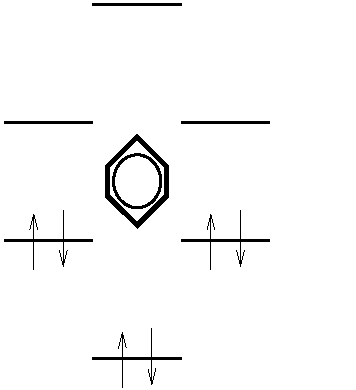
\includegraphics[scale=0.5,clip=]{benz-eht}}
  \subfigure[]{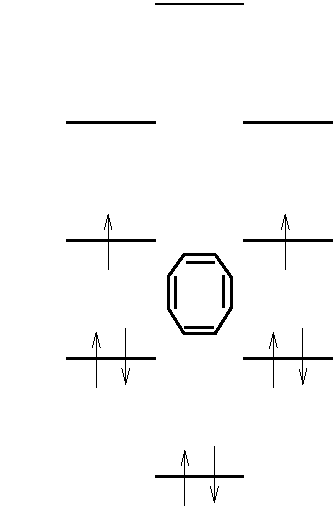
\includegraphics[scale=0.5,clip=]{cyklooktene}}
\caption{Molecular orbital diagrams  for the $\pi$-electron system in (a) 
benzene and (b) in cyclotetraoctene.}
\label{fig:huckeldiag}
\end{figure}
Stated in another way; the angular part of a wave function in a circular
potential would
correspond to $\Psi(\theta)=e^{i|m|\theta}$, where $\{m \in \mathrm Z\}$ and
$0\leq\theta\leq 2\pi$. 
Since  two electrons can occupy each
orbital, the degeneracy for $\{|m|~|~m \in \{0,\pm
1,\pm 2,\ldots\}\}$ is $2,4,4,\ldots$, from which the H\"uckel rule follows:
$4\sum_{i=1}m_i+2=4n+2$.

The $\pi$-orbitals thus have a shell-like structure.
As each orbital can occupy two electrons it takes precisely ($4n+2$)
electrons to fill a shell. In the case of benzene, which is the
prime example of an aromatic molecule, there are 6 $\pi$-electrons filling up
the three lowest molecular orbitals. All of these orbitals are bonding,
whereas the three unoccupied orbitals are anti-bonding, 
explaining much of the great stability of benzene.

\section{Ring currents}
\label{sec:rc}
The shell structure of aromatic molecules also has a profound effect on the
magnetic properties of these systems. Aromatic molecules are known to exhibit
an exalted diamagnetic response to external magnetic fields. When an aromatic
molecule is subjected to an external magnetic field perpendicular to the
molecular plane, the induced current can flow not only in the individual 
chemical bonds but also around the conjugated $\pi$-system, giving rise to a
non-vanishing net current. This ring current
is directed so that the secondary induced magnetic field from the current is
directed opposite to the external field, as seen in \Fig{fig:ringcurr}. From
this figure it can be seen that the net magnetic field is decreased on the
inside of the ring and enhanced on the outside of the ring. This effect is
sometimes visible in NMR experiments \cite{Abraham:65,Wuthrich:82}, 
where the outer protons
are deshielded compared to normal values for aliphatic molecules. A nucleus
on the inside of the ring would experience a stronger magnetic shielding.
\begin{figure}[b]%[H]
\centering
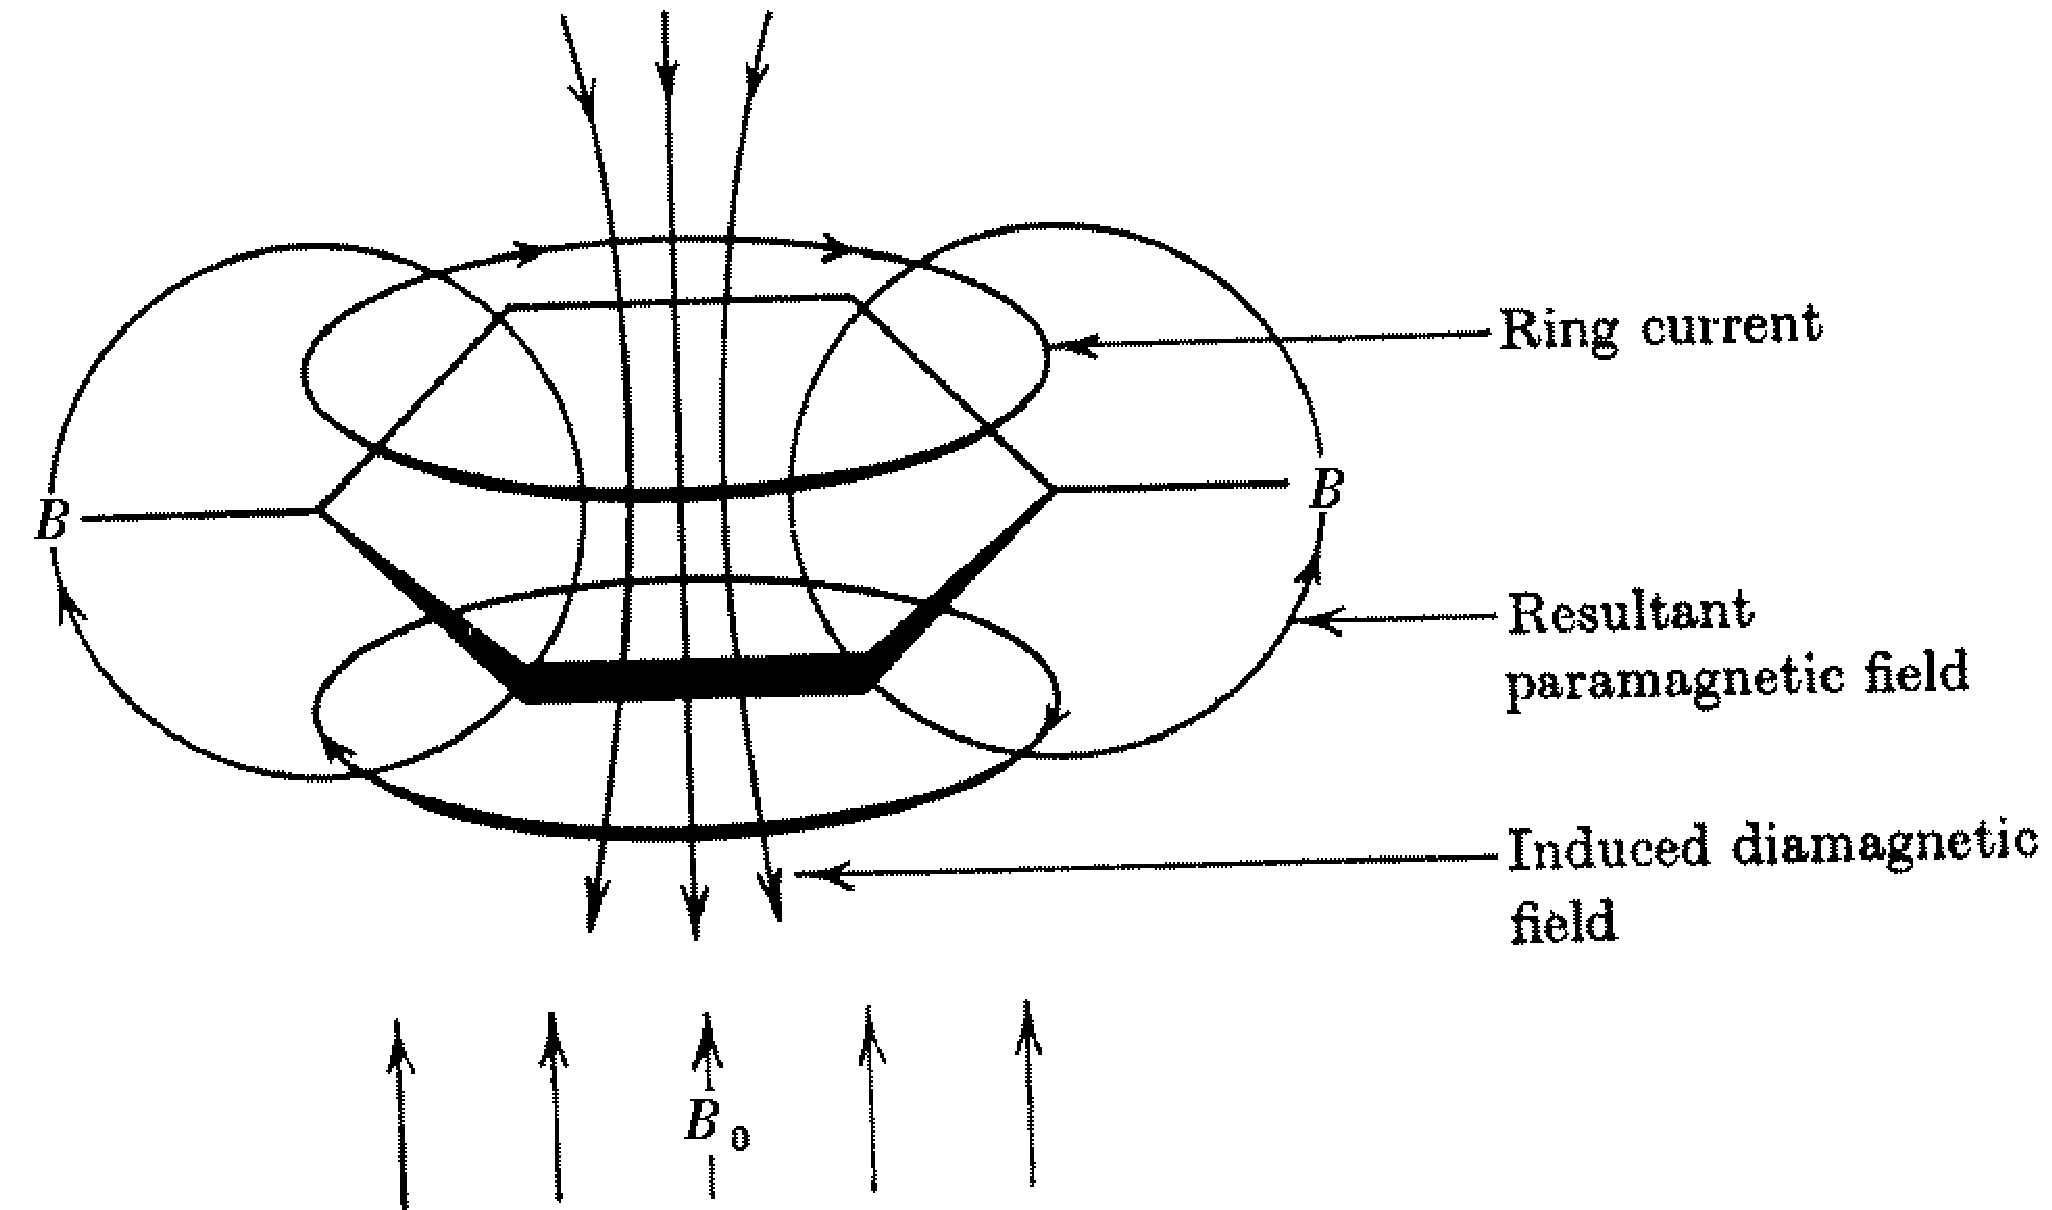
\includegraphics[width=7.5cm,clip=]{ringcurr}
\caption{Schematic picture of the induced ring current in benzene.}
\label{fig:ringcurr}
\end{figure}

\subsection{Orbital contributions to the ring current}
The diamagnetic ring-current effect has been neatly explained in terms of
symmetry by Steiner and Fowler \cite{Fowler:01a,Fowler:01b}, and we shall follow
their arguments here. For simplicity we shall only consider electrons in an
independent-particle model for which the eigenvectors are the MOs and
eigenvalues are the orbital energies.  Using perturbation theory, the 
first-order change to an occupied orbital $\psi_n^{(1)}$ can be partitioned 
into a paramagnetic and a diamagnetic part 
\begin{equation}
\psi_n^{(1)}=\psi_n^{(p)}+\psi_n^{(d)}=-\oover{2}\sum_{a>N}\psi_a
\frac{\bra\psi_a|\hat{l}|\psi_0\ket}{\epsilon_a-\epsilon_n}\cdot\mbf{B}
+\oover{2}\mbf{d}\times\sum_{a>N}\psi_a
\frac{\bra\psi_a|\hat{p}|\psi_0\ket}{\epsilon_a-\epsilon_n}\cdot\mbf{B},
\label{psipd}
\end{equation}
where the summation runs over all virtual orbitals. When this equation is used
in conjunction with \Eq{Jreal}, 
it can be shown that $\psi_n^{(p)}$ gives rise to
the paramagnetic contribution to the current and $\psi_n^{(d)}$ gives rise 
to the diamagnetic current. 
From \Eq{psipd} it is immediately clear that the largest contributions to the 
perturbed wave function come from the low-lying unoccupied orbitals. 
Furthermore, the amplitudes are affected by
the symmetry of the orbitals and operators. The angular momentum operator
$\hat{l}$ spans the irreducible representations (irrep), $\Gamma$, for
rotational symmetry, $R$, of the molecular point group, and the linear momentum
operator, $\hat{p}$, spans the translational  symmetry $T$. When the magnetic
field is perpendicular to the molecular plane, only $R_\parallel$ and
$T_\perp$ need to be considered as the other components are trivially zero.
Thus, the only amplitudes which are non-zero, are those for which 
\begin{equation} 
A_1\in\Gamma=\{\Gamma_{\psi_a}\otimes\Gamma_{\{\hat
l,\hat p\}}\otimes\Gamma_{\psi_0}\},
\end{equation} 
where $A_1$ is the totally symmetric irreducible representation. In other
words, if the direct product of the orbitals and the operator does not span the 
totally symmetric component, the integral vanishes.
In aromatic molecules, the first accessible transition is to the lowest
unoccupied molecular orbital (LUMO) via a translational excitation, giving
rise to a large contribution to the diamagnetic response (diatropic current). 

In contrast, molecules with a conjugated $\pi$-system containing $4n$
electrons behave completely differently. In such systems the largest
contributions to the current come, not from the translational transitions, but
from rotational excitations making the overall current paratropic. In these
molecules, there are usually substantial contributions from
translational transitions making the paramagnetic response less
pronounced. Molecules sustaining paratropic currents are usually classified
as antiaromatic. Antiaromatic molecules are much less common than aromatic
molecules. Examples of antiaromatic molecules are cyclotetraoctene (see
\Fig{fig:huckeldiag}) and cyclodecatrienetriyne, which is discussed more in
detail in \citetalias{Juselius:t01a}.

These arguments are of course simplifications, based on some 
simple H\"uckel-type Hamiltonian, but the general ideas are valid. In
\Ch{ch:gimic} a method of calculating the current for the full quantum
mechanical system is derived. Before doing so we shall look at some
qualitative methods to estimate the ring current.

\section{Types of aromaticity}
As pointed out earlier, aromaticity is an elusive phenomenon. As a result, in
the pursuit to classify, quantify and understand the subject, aromaticity has
been given many subclasses. The following section presents the most common
types of aromaticity, with the emphasis on the ring currents. Henceforth, I
shall use the word aromaticity as a synonym for ability to sustain a ring
current.

\subsection{Normal aromaticity}
Benzene is the epitome of aromaticity. Not only was it the first aromatic
molecule to be discovered \cite{Faraday:1825}, but it has almost every
conceivable characteristic of aromaticity. Benzene has unusually high
stability, low reactivity, no bond length alternation in the carbon
framework, high magnetic susceptibility, highly deshielded proton shifts
corresponding to a strong ring 
current \cite{Juselius:t99,Juselius:MSc,Lazzeretti:00}. The
induced current in benzene is visualized in \Fig{fig:benz-curr}.
Figure~\ref{fig:benz-curr}(a) shows the current in the molecular plane
containing the nuclei. By inspection it is easy to see that the net current is
nearly zero due to cancellation, and that most of the currents are localized
in the $\sigma$-bonds. On the other hand, \Fig{fig:benz-curr}(b) shows the
current in a plane approximately 0.5 � above the molecular plane,
in the region of large $\pi$-electron density, where the ring-current effect
is very clearly visible.
\begin{figure}%[H]
\begin{center}
\subfigure[]{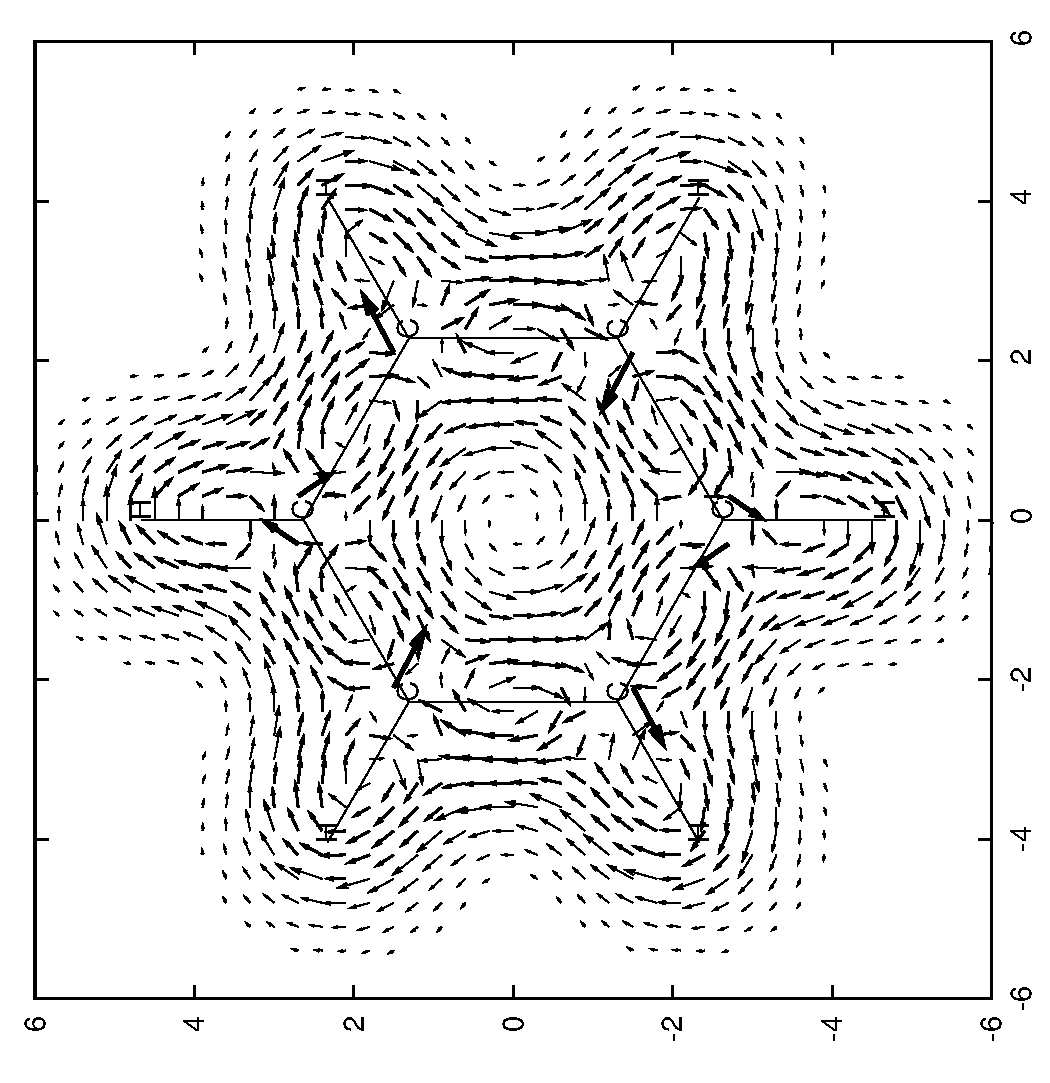
\includegraphics[clip=0,scale=0.36,angle=-90]{benzene_0au}}
\subfigure[]{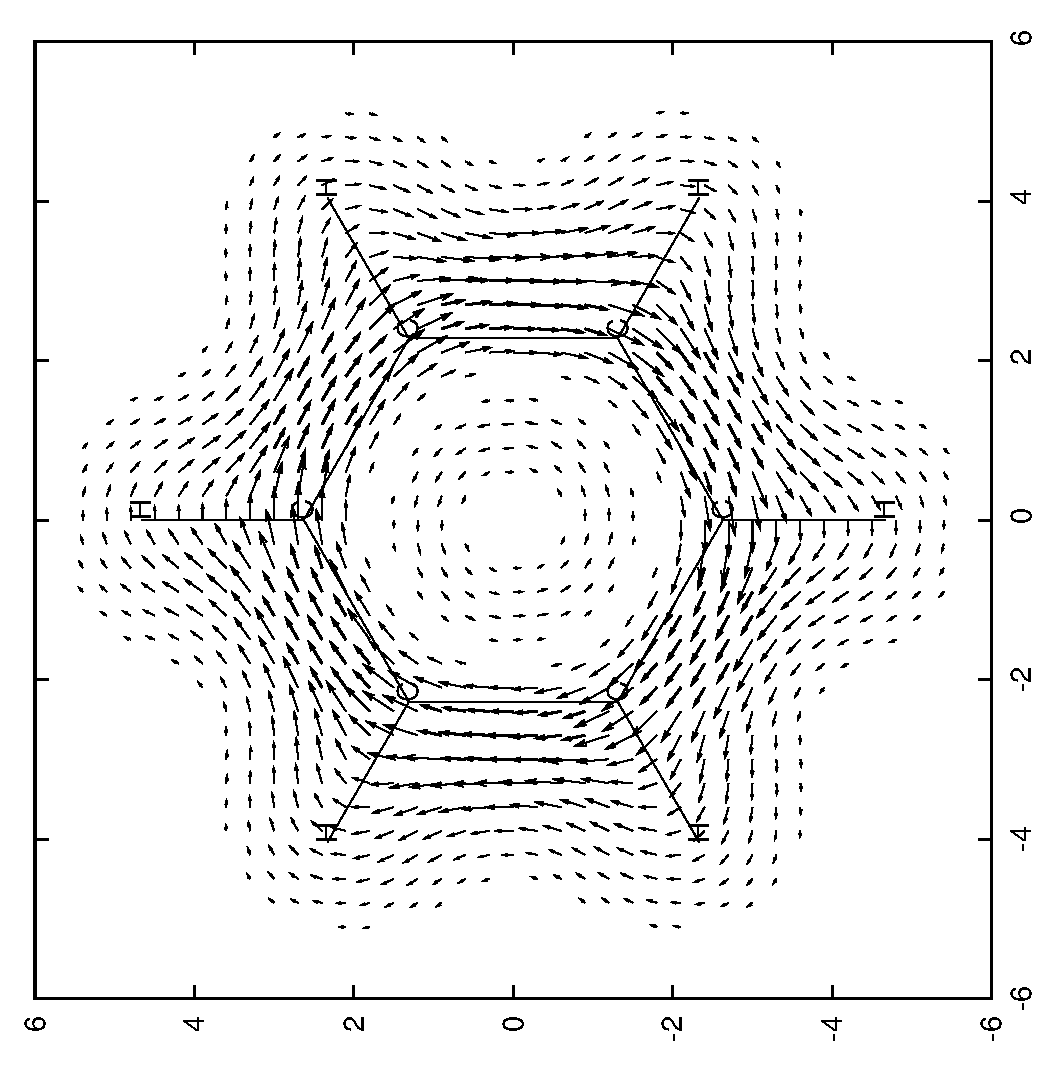
\includegraphics[clip=0,scale=0.36,angle=-90]{benzene_1au}}
\caption{Induced current density in benzene calculated at
the HF-SCF/TZP level.
Figure (a) shows the current density in the plane defined by the nuclei, and
Figure (b) shows it 1 Bohr above the molecular plane. The magnetic field 
is directed perpendicular to the molecular plane.}
\label{fig:benz-curr}
\end{center}
\end{figure}

In more complicated aromatic molecules, consisting of one or more fused rings,
questions arise, not only regarding the ring current, but also about the
aromatic pathway. In simple fused molecules like naphthalene the question is
easy to answer, but in more complicated systems like porphyrins or coronenes
the answer needs a careful analysis \cite{Juselius:t00,Juselius:t00a,
Juselius:t04}.
%The ring current in hexabenzocoronene is shown in \Fig{fig:coronene}. 
It is
interesting to note that the classical law of Kirchoff \cite{Ohanian:89} 
also holds in
molecular systems. The need to understand the aromatic pathways in molecules
is not only of academic interest, but can also be of importance
to, for example, molecular transistors.%\cite{transistor}.

\subsection{Antiaromaticity}
Molecules classified as antiaromatic have $4n$ $\pi$-electrons, and thus
show a paramagnetic response to magnetic fields. Antiaromatic molecules are
not very common, as $4n$ $\pi$-electrons usually constitute an open
$\pi$-shell. Prime examples of a closed-shell antiaromatic molecules are 
cyclobutadiene and cyclodecatrienetriyne \cite{Pople:66,Juselius:t01a}.

\subsection{$\sigma$-aromaticity}
Ring currents are not only confined to $\pi$-electrons as in organic molecules.
Certain inorganic molecules can sustain ring currents also in the
$\sigma$-framework. This phenomenon is probably due to low-lying $\sigma^*$
and $\pi^*$
orbitals in metallic rings.
An example of a $\sigma$-aromatic molecule is 
Al$_4^{2-}$\cite{Li:01,Lin:t04} which has been observed experimentally.

\subsection{Homoaromaticity}
Homoaromatic molecules are classified as compounds that show aromatic
character even though the molecular conjugation is interrupted by single bonds
\cite{Winstein:59,Childs:84,Williams:01}. The concept of homoaromaticity was
introduced more than 40 years ago and is still of interest
\cite{Williams:01}. A family of potentially homoaromatic molecules can be
derived from cyclic and conjugated $(4n+2)\pi$-electron hydrocarbon species by
inserting a CH$_2$ unit into the molecular ring.  
The best-known example of
this kind of species is probably the homotropylium cation (C$_8^{}$H$_9^{+}$)
which can be considered as an aromatic C$_7^{}$H$_7^{+}$ ion with an
additional CH$_2$ unit. An interesting feature of homo-aromatic aromatic
molecules is that the ring current does not follow the molecular framework,
but can ''leap`` through space at the junction of the CH$_2$
group \cite{Winstein:59,Childs:84,Williams:01,Juselius:t03}, illustrated
schematically for the homotropylium cation in \Fig{fig:homo-curr}.
\begin{figure}[!hb]%[H]
\begin{center}
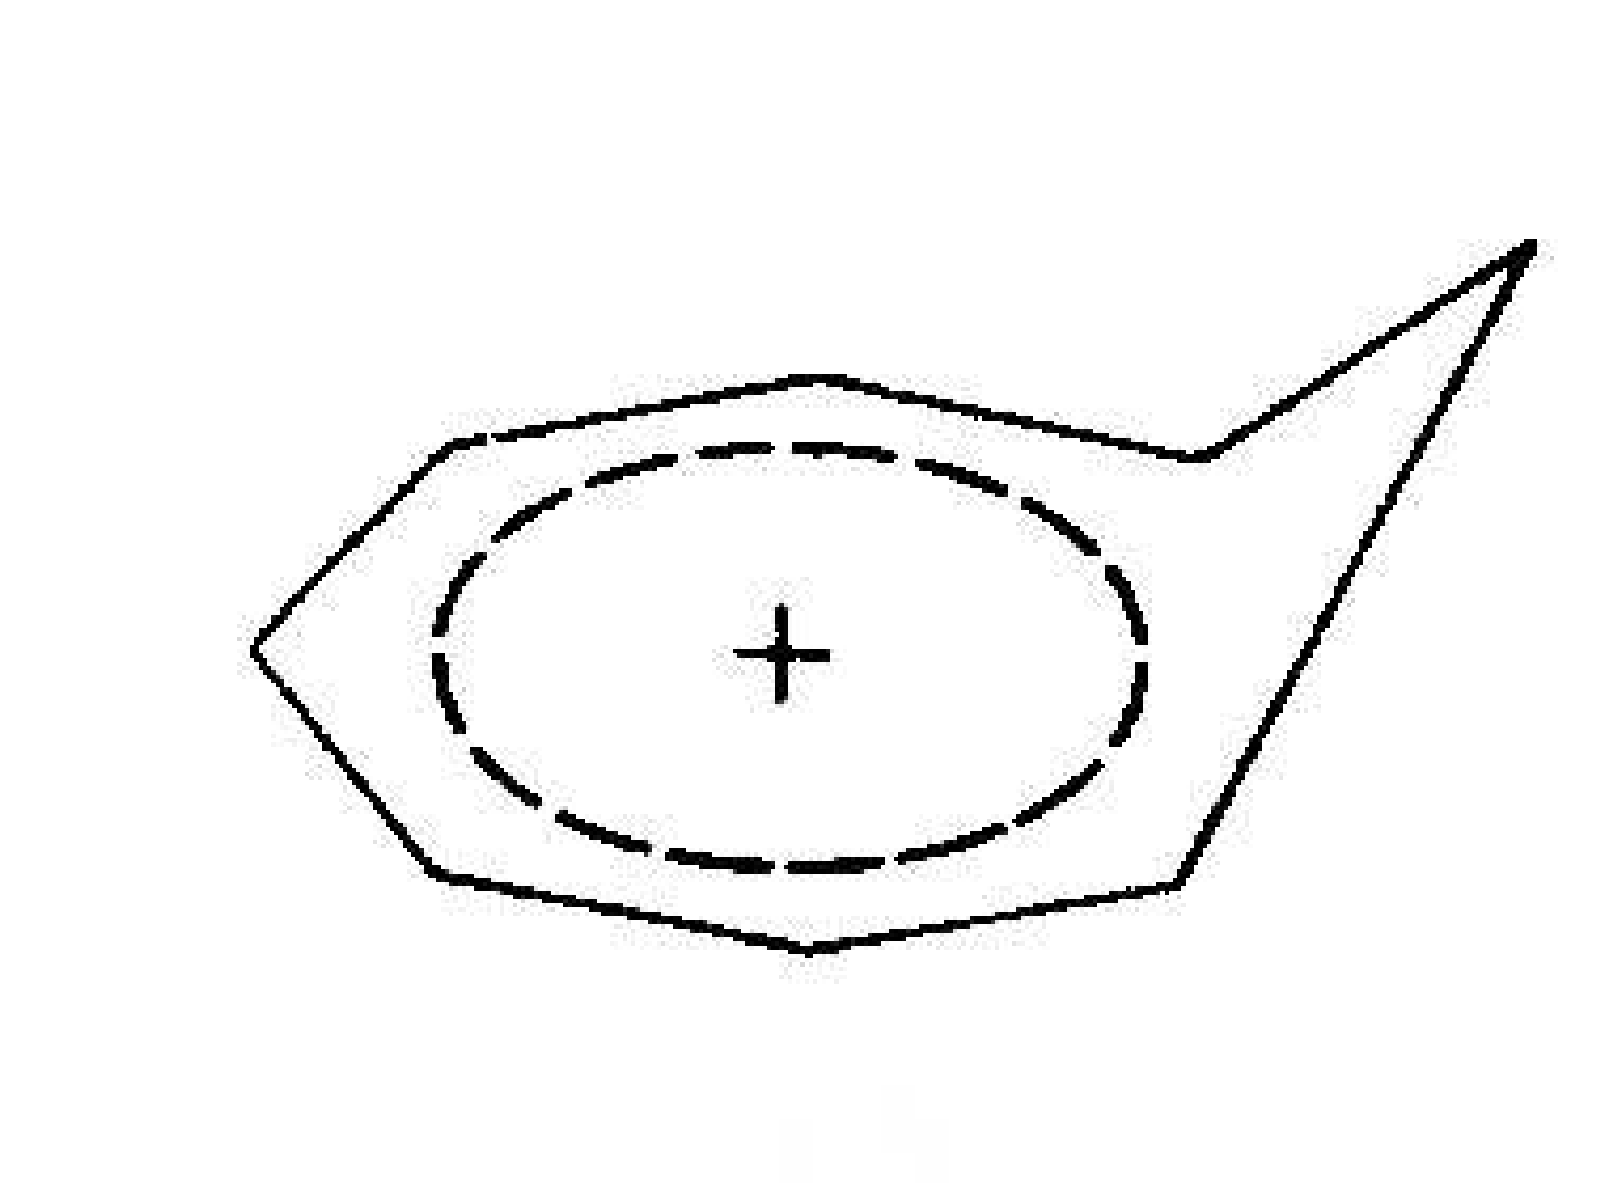
\includegraphics[clip=0,scale=0.10,angle=0]{homotropylium}
\caption{Schematic illustration of the ring current in the homotropylium
cation.}
\label{fig:homo-curr}
\end{center}
\end{figure}

\subsection{Spherical aromaticity}
A very interesting group of systems are cage molecules of high symmetry. 
Hirsch \cite{Hirsch:00} initially proposed a revised aromaticity rule for molecules
of icosahedral symmetry, in particular fullerenes \cite{Chen:01}.  
In contrast to the normal
H\"uckel ($4n+2$) rule for planar systems, molecules of $I_\mathrm{h}$
symmetry show complete filling of the electronic shell for $2(n+1)^2$
$\pi$-electrons. This rule has been
verified \cite{VanLier:02,Buehl:01,Buehl:98} for molecules like, C$_{20}^{2+}$,
C$_{60}^{10+}$ and C$_{80}^{8+}$. The rule for spherical aromaticity has later
been extended to include other highly symmetrical molecules belonging to the
$T_\mathrm{d}$ and $O_\mathrm{h}$ symmetry point
groups \cite{Chen:01,Hirsch:01,Hirsch:02}. The induced current of C$_{60}$ and
C$_{60}^{10+}$ are shown in \Fig{fig:shpere-curr}.

Another interesting property of these molecules, both spherical aromatic or
not, is to act as magnetic Faraday cages in the sense that the shielding is
constant within the shell \cite{Lounila:94,NMRBOOK:04,Lazzeretti:00,
Johansson:04}.
\begin{figure}
\begin{center}
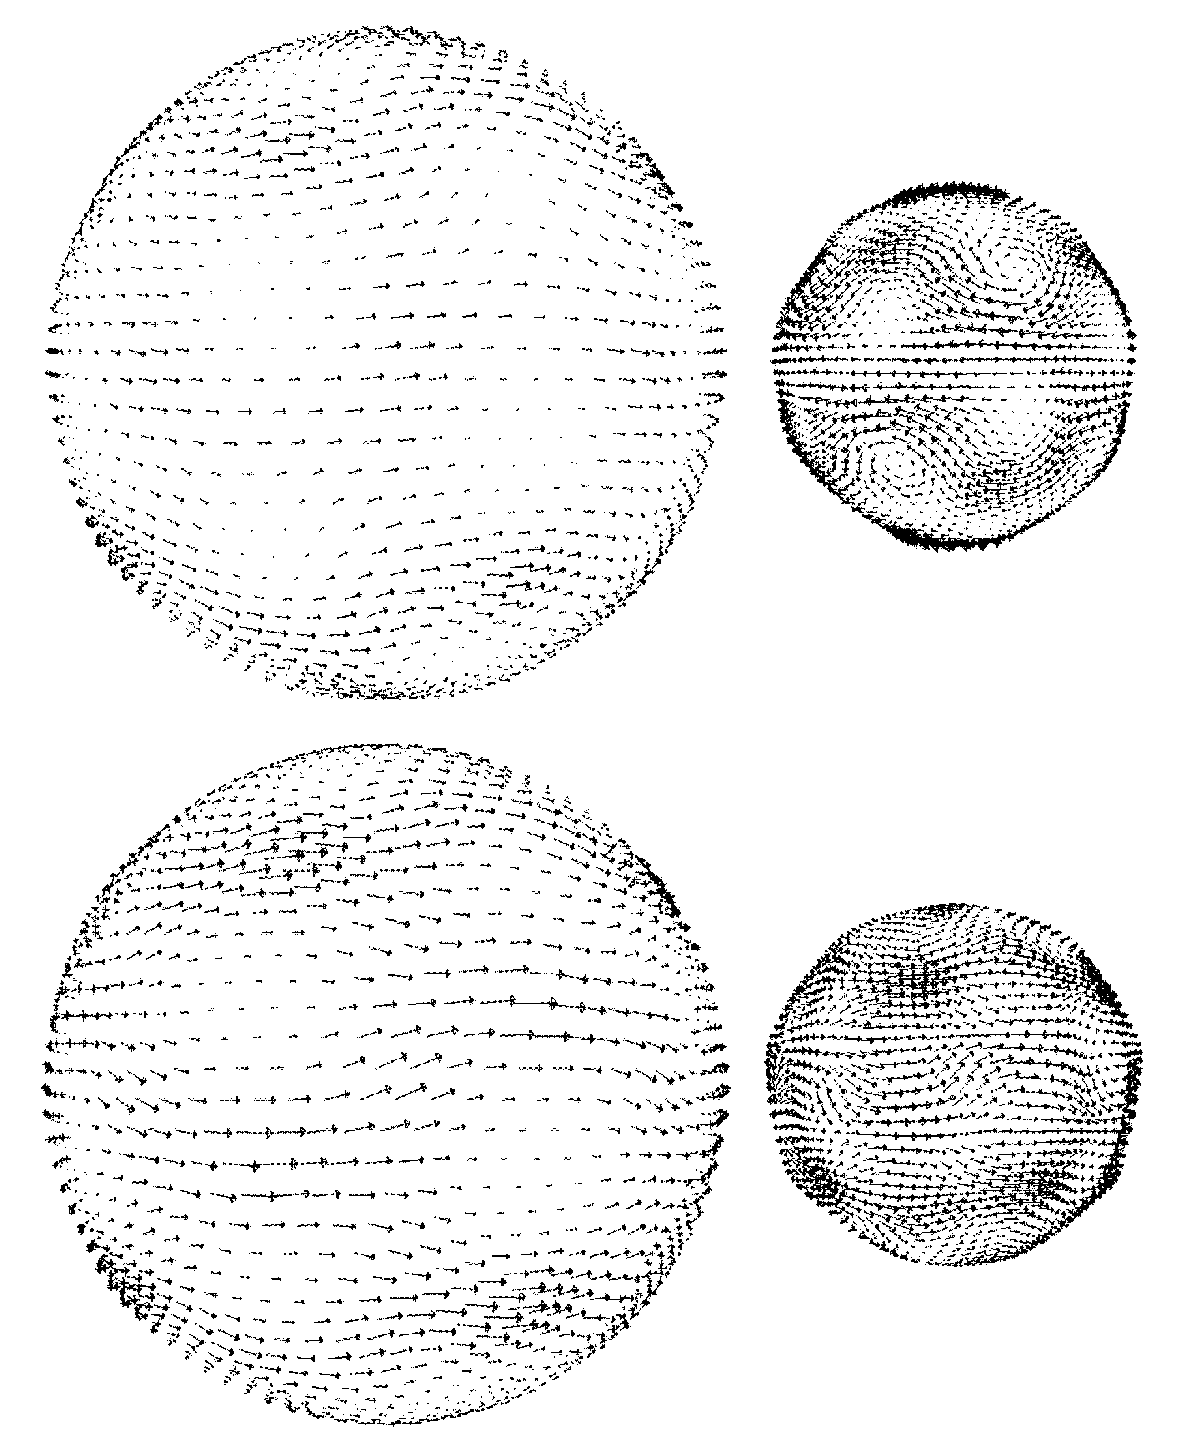
\includegraphics[clip=0,scale=0.4,angle=0]{C60}
\caption{The induced currents in neutral (top), and +10 charged (below)
fullerene, 1 � above (right) and below (left) the surface. The magnetic field
is directed along the figure plane, from top to bottom.}
\label{fig:shpere-curr}
\end{center}
\end{figure}

\subsection{M�bius aromaticity}
As a curiosity, Heilbronner \cite{Heilbronner:64} predicted that singlet
[$4n$]annulenes could be aromatic in certain twisted conformations. If the
carbon $p$-orbitals lie on a M�bius-like surface, the annulene should be able 
to sustain a diatropic current. Schleyer {et al.} have studied a number of
such M�bius annulenes and found them to be aromatic according to the NICS
aromaticity index \cite{Schleyer:02} ({\em vide infra}).  

\section{Nucleus-independent chemical shifts}
A very simple method of estimating the aromaticity through the strength
of the ring current was proposed by Schleyer {\em et
al.}\cite{Schleyer:96b,Subramanian:96} . The method lends its idea from the
aromatic shift observed in $^1$H NMR experiments and
calculations \cite{Abraham:65}.  However, the aromatic contribution to the
proton shielding is often relatively small and the proton shieldings also
depend significantly on other factors, such as the size of the current circuit,
the number of electrons, and the substituents.  Thus, the indirect measurement
of the strength of the ring current by detecting the proton shieldings does not
provide a general method for determining the degree of aromaticity.

Instead of using protons, which have fixed positions in
molecules, one calculates the NMR shielding for a ''ghost'' nucleus which 
carries
no charge, and no basis functions. Such a ghost atom has no effect on the
electronic structure of the molecule and can be placed anywhere in the
molecule to probe the magnetic shielding. This approach is called the 
Nucleus-Independent Chemical Shift (NICS) method, and has in recent times 
become a very popular tool of assessing molecular aromaticity. 

In the original proposal \cite{Schleyer:96b} one calculates the shielding 
tensor for one ghost
atom located at the center of the molecular ring. For topological reasons the
magnetic exaltation is largest near the center of the ring 
(see \Fig{fig:ringcurr}).
Judging from the NICS value one should in principle be able to estimate 
the strength of the current, and say whether a molecule is
aromatic or not.

There are a number of problems with the NICS 
approach \cite{Lazzeretti:04,Juselius:t01a,Juselius:t03}. 
The first problem is the lack of a
reference. Since one cannot simply turn off the current to get a non-aromatic
NICS reference value, one must either rely on NICS values for other molecules,
or chemical intuition. Neither approach is very satisfactory in terms of
reliability.  In general, the NICS values are not transferable from one group
of
molecules to another \cite{Buehl:98}. They can  be used as a relative measure
of the aromaticity for closely related molecules, but the NICS values do not
provide any accurate information about the strength of the ring current, since
the shielding at the center of the molecule depends on both the size of the
circuit and the current strength. The second problem is that there is usually
substantial electron density at the NICS point, which affects the
shielding through both electrostatic and quantum effects.  Some of these
problems have been acknowledged, and contemporary NICS calculations are often 
carried out using two NICS values. The NICS(0) is calculated in the original
NICS point, and an additional NICS(1) is calculated 1 atomic unit (0.52~�)
above the plane. Certain molecules, {\em e.g.}
Al$_4^{2-}$\cite{Lin:t04}, have diamagnetic short-range shielding, but
overall paramagnetic long-range shielding. For such molecules both NICS(0),
and NICS(1) values still give faulty answers regarding the aromaticity.

Recently the NICS method has been used to analyze the
the so-called anisotropy effect on fragments in NMR 
experiments \cite{Klod:01,Klod:02,Heine:04}. 
Larger molecules can be considered to be built from a number of functional
groups. The shieldings in functional groups can be strongly affected by other
groups near-by, causing difficulties in resolving NMR spectra correctly.
Functional groups containing double- or triple bonds and, in particular, 
aromatic rings give rise to highly anisotropic shieldings. In the method of
Klod and Kleinpeter \cite{Klod:01}, NICS values are calculated on a three
dimensional grid. By visualizing the isotropic shieldings on isosurfaces the
long-range shielding effects of functional groups can be better understood.
Using this method they have been able to resolve the NMR spectra for a number of
stereo-isomers.

%Klod, Kleinpeter J. Chem. Soc. Perk. Trans. 2 (2001) 1893 | (2002) 1506.

\section{Aromatic ring-current shieldings}
\begin{figure}%[H]
\centering
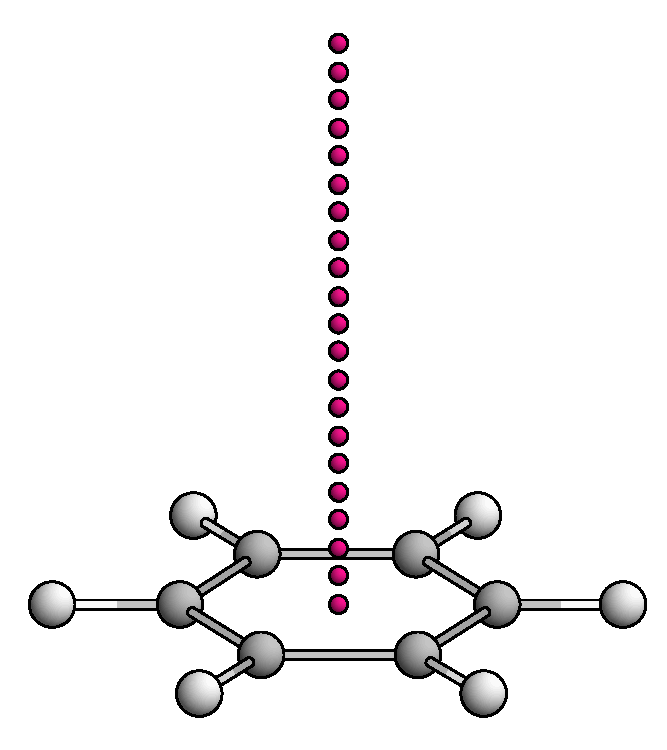
\includegraphics[scale=0.35,angle=-90,clip=]{benzarcs}
\caption{A set of ARCS probes in the center of, and perpendicular to, 
the molecular plane in benzene. Using a single point in the molecular plane
would correspond to the NICS(0) index.}
\label{fig:arcsline}
\end{figure}
To overcome some of the problems with the NICS approach, we 
devised a new method, called the Aromatic Ring-Current Shieldings (ARCS)
method, in \citetalias{Juselius:t99}. 
Instead of probing only {\em one} point in space, a {\em
set} of points along a line perpendicular to the aromatic ring are probed (see
\Fig{fig:arcsline}). Calculating the nuclear magnetic shielding along this
line gives the shielding as a function of distance from the center of the
molecule, $\sigma(r)$. As discussed in section~\ref{sec:rc}, a ring current
circulating in a molecule gives rise to a strong magnetic field which affects
the long-range shielding of the probes. Making the assumptions that the
current is of a classical nature and that the current loop is circular and
infinitely thin, the long-range shielding can be analyzed in terms of
classical electrodynamics. Strictly speaking, the last two assumptions are not
necessary but simplify the treatment considerably. Using the Biot-Savart law
\cite{Arfken:85}, the long-range shielding can be related back to the strength
of the current circulating in the molecule.

%The induced ring current leads to an additional (induced) magnetic field 
%that can be observed as a long-range magnetic shielding contribution. 
%In our previous work 
%\cite{Juselius:t99,Juselius:t00,Juselius:t00a,Juselius:t01,Juselius:t01a,Berger:01,Juselius:t03},
%we estimated 
%ring-current strengths from the shape of the long-range magnetic 
%shielding function based on Biot-Savarts law for an infinitely
%thin and circular conductor ring.

The Biot-Savart expression for the magnetic field strength ({\bf B})
in the vicinity of a thin wire carrying a current $I$ is 
\begin{equation}
\label{eq1}
{\bf B} =\frac{\mu_0~I}{4\pi} \int \frac{d{\bf l}\times{\bf r}}{r^3},
\end{equation}
where ${\mu}_0$ is the permeability of vacuum, $d{\bf l}$ is a small length
element of the conductor, $r$ is the distance from the wire, and ${\bf r}$ is
the radial vector from $d{\bf l}$ to the probe. Assuming an
infinitely thin circular wire, the primitive function of \Eq{eq1} along
the symmetry axis of the loop becomes
\begin{equation} 
\label{eq2}
B(z)=\frac{\mu_0~I}{2}\frac{R^2}{(r^2+R^2)^{3/2}}  = -\sigma(r) B_{ex},
\end{equation}
where $R$ is the radius of the current loop, $r$ is taken to be the
perpendicular distance from the loop center. For large $r$-values, 
\Eq{eq2} yields the correct asymptotic behavior of $r^{-3}$ as expected for
a magnetic dipole. If the assumptions about the current loop hold, the induced
magnetic field is related linearly to the isotropic nuclear magnetic shielding 
function along the $r$-axis, $\sigma(r)$, for a given external magnetic field 
$B_{ex}$. 

Differentiating \Eq{eq2} with respect to the external magnetic field, yields
the relation between the isotropic nuclear magnetic shielding and the
derivative of the induced current with respect to the applied magnetic field:
\begin{equation}
\label{eq3}
\sigma(r) = -\frac{\mu_0}{2} \frac{\partial I}{\partial B_{ex}} 
\frac{R^2}{(r^2+R^2)^{3/2}} .
\end{equation}
The strength of the induced ring current for a given magnetic field can  
be obtained as:
\begin{equation}
\label{eq4}
I = \frac{\partial I}{\partial B_{ex}} B_{ex}.
\end{equation}
Calculating $\sigma(r)$ for a number of $r$-values 
in the range $r=[0,r_{max}]$, the induced current derivative  
($\frac{\partial I}{\partial B_{ex}}$) and the loop radius ($R$) 
can be deduced from the long-range part of the shielding function by fitting
to \Eq{eq3}. 
Typical values for $r_{max}$ are 30-60 Bohr, depending on the loop size. 
For small values of $r$, the shieldings do not obey the Biot-Savarts 
law for the circular model, as electrostatic and quantum effects of the
electron density start to play a role. Also, at short distances, the
approximation that the current loop is infinitely thin, is not very good.
In order to get reasonable and stable fits it is necessary to use a cut-off,
$r_{min}$, for the shielding function close to the ring. 
The results are not very sensitive to the choice of 
$r_{min}$ as long as it is outside the electron charge distribution. 
Typical $r_{min}$ values are about 3-5 Bohr (1.50-2.50 �). 
In many respects the ARCS method can be viewed as an experimental procedure in
a theoretical framework. 
\begin{figure}%[H]
\begin{center}
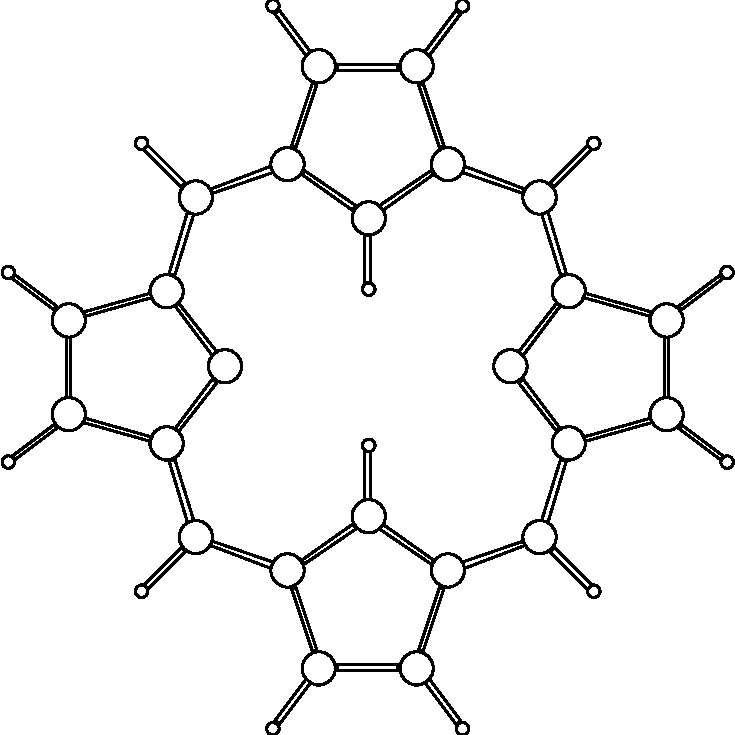
\includegraphics[clip=0,scale=0.4,angle=-90]{t-PH2}
\caption{The molecular structure of free-base porphyrin.}
\label{fig:t-PH2}
\end{center}
\end{figure}

The degree of aromaticity is usually assumed to be
proportional to the strength of the induced ring current which is a measure of
the delocalization of the $\pi$-electrons \cite{Elvidge:61}.  The degree of
aromaticity of any molecule, deduced from the calculated ARCS data, can then
be compared regardless of the size of the aromatic path. More precisely, the
shieldings are proportional to the derivative of the current strength with
respect to the applied magnetic field, while the ring current depends on the
field strength. Figure~\ref{fig:PH2-arcs} shows the result of an ARCS calculation
for free-base porphyrin.

\begin{figure}[b]%[H]
\subfigure[]{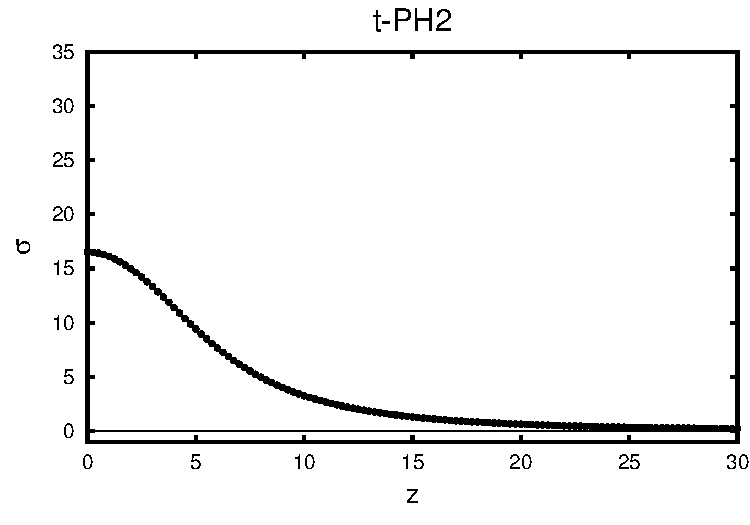
\includegraphics[width=7.5 cm,clip=]{arcs-t-PH2-dat}}
\subfigure[]{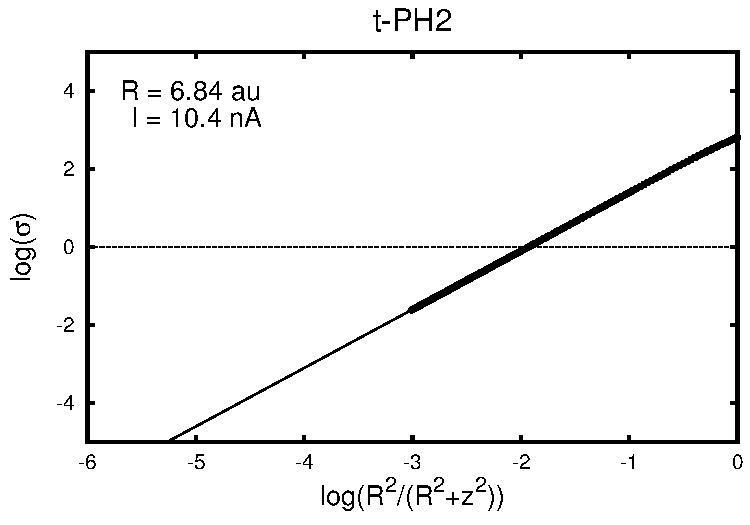
\includegraphics[width=7.5 cm,clip=]{arcs-t-PH2-fit}}
\caption{The calculated ARCS functions (a) for free-base porphyrin (in ppm)
and (b) the logarithmic fit of the ARCS functions to Eq. (\ref{eq3}).}
\label{fig:PH2-arcs}
\end{figure}

While the ARCS method has proved to be a very useful tool to calculate the
over-all strength of the ring current in molecules, it cannot convey any
details about the structure of the currents in molecules. The need to obtain
more detailed information about the currents becomes evident for more
complicated molecules consisting of multiple or fused aromatic rings. For
example free-base porphyrin (see \Fig{fig:t-PH2}) consists of four pyrrole
groups connected by conjugated bonds to form a macro cycle, and has ring
currents which are rich in detail (see Articles II, III and VII in the
Appendix). In an attempt to analyze this underlying structure we developed 
a method called Planar ARCS (PARCS).

In the PARCS approach, the shielding function is calculated in a
plane parallel to the molecular plane at a distance from it.
The PARCS data provides some information about anisotropies
in the ring currents, but it does not directly yield any information
about the fine structure of the currents.
It is, however, possible to manipulate the PARCS data in order to get
more detailed information about current paths.
The calculated two-dimensional PARCS functions can be expanded in
two-dimensional momentum functions analogously to
the expansion in spherical harmonics in the three-dimensional case
\begin{equation}
\label{parcseq3}
\phi(x,y)=\sum_i f_i(r)\chi_i(\theta),
\end{equation}
where $\chi_i(\theta)$ are angular functions {\it i.e.}
$s$, $p_x$, $p_y$, $d_{x^2-y^2}$, and $d_{xy}$, while $f_i(r)$
are the corresponding radial parts.
The radial functions for the first few angular functions can be obtained
by numerical integration and Gram-Schmidt orthogonalization.
The projected PARCS functions are obtained as
\begin{equation}
\label{parcseq4}
\tilde\varphi(r,\theta)=\varphi(r,\theta)-\sum_k
\frac{\int\chi_k(\theta)\varphi(r,\theta)d\theta}{\int\chi_k^2(\theta)d\theta}
\chi_k(\theta)~.
\end{equation}

By projecting out the dominating $s$-term and eventually some of
the higher-order terms from the two-dimensional PARCS function,
the underlying fine structure of the ring current is revealed. 
The results of the PARCS analysis for free-base porphyrin are shown in 
\Fig{fig:parcs}. Figure (b) clearly shows the existence of stronger local 
currents in the pyrrole units with an inner hydrogen.

\begin{figure}%[H]
\begin{center}
\subfigure[]{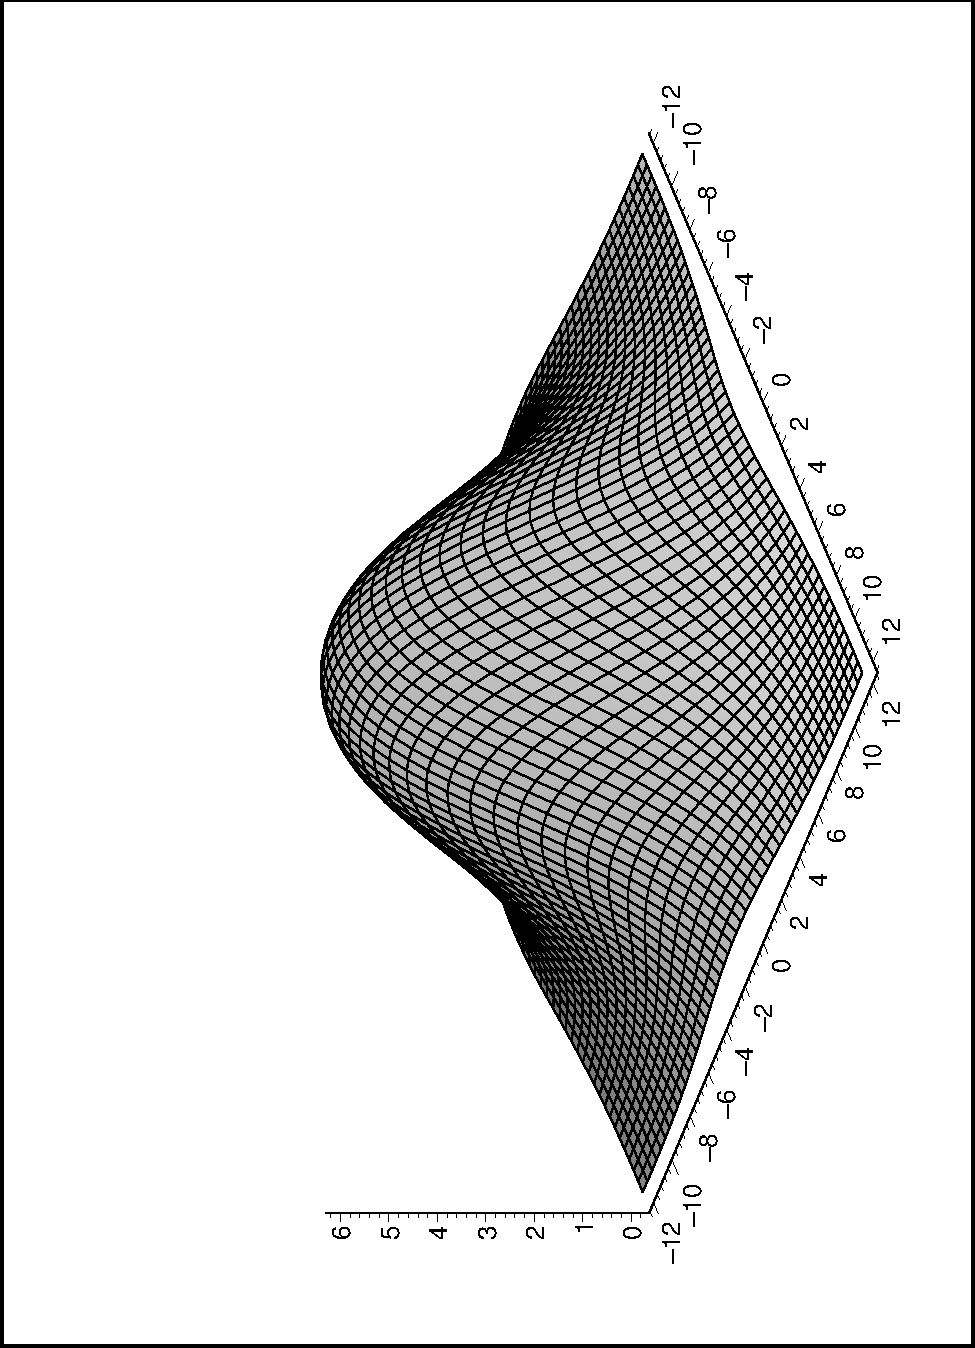
\includegraphics[clip=0,scale=0.32,angle=-90]{t-PH2_parcs}}
\subfigure[]{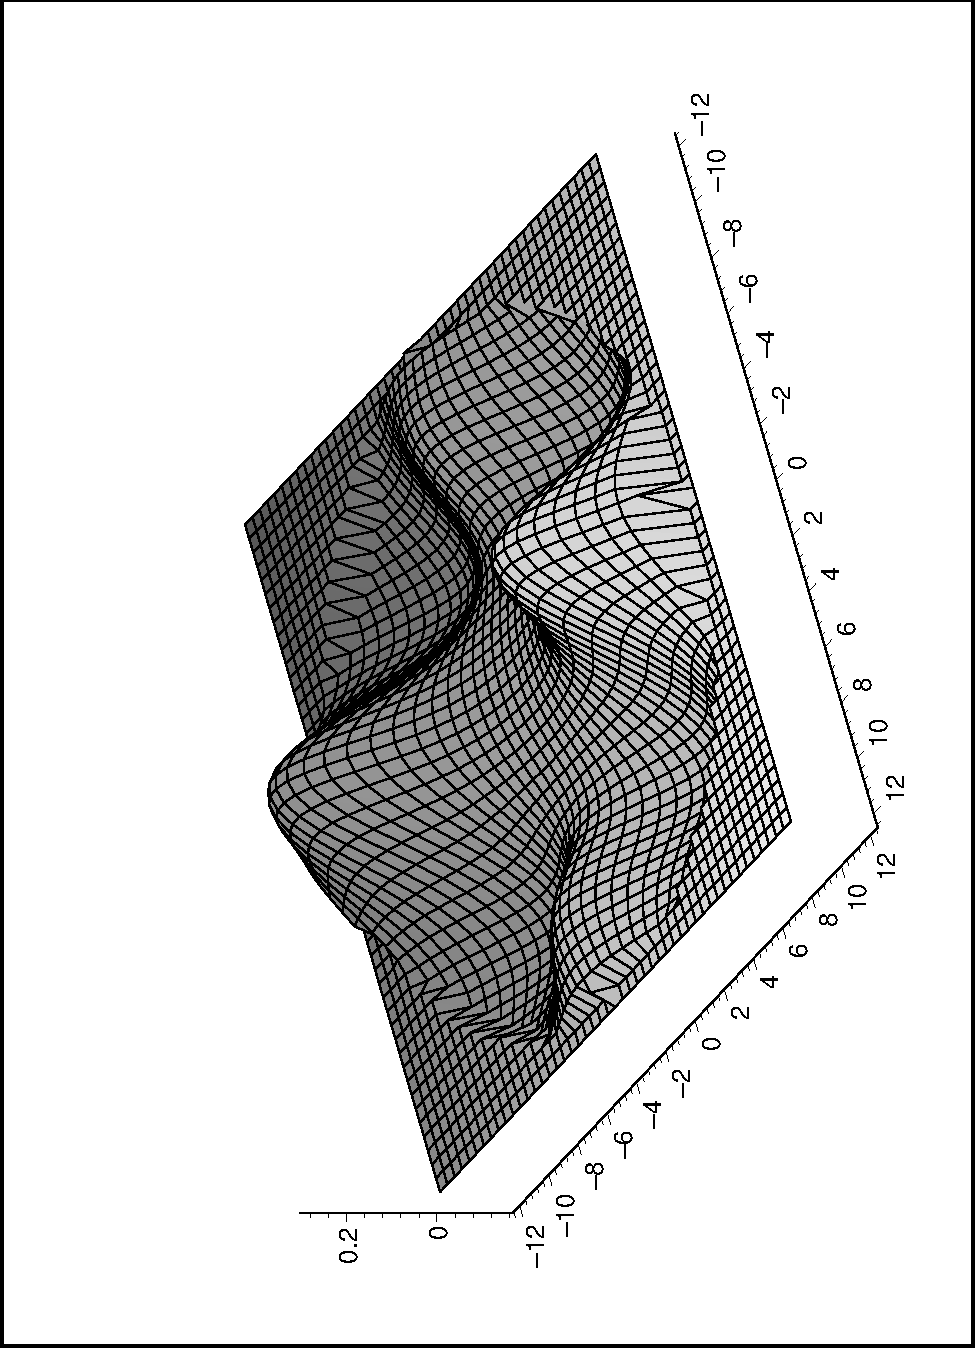
\includegraphics[clip=0,scale=0.32,angle=-90]{t-PH2_parcsint}}
\caption{(a) The nuclear magnetic shieldings for free-base porphin 
calculated at a distance of 7 Bohr from the molecular plane. (b)
The PARCS function after the circular
symmetric part has been projected out.
}
\label{fig:parcs}
\end{center}
\end{figure}

\chapter{Calculation of magnetically induced currents}
\label{ch:gimic}
We shall now turn from qualitative ring-current models to methods for
explicitly treating the magnetically-induced quantum-mechanical current 
density. The methods presented here are concerned with the time-independent
current density in closed-shell molecules. 

The first calculations of ring currents were based on simple model
Hamiltonians of H\"uckel type. Some of the earliest work goes back to Pauling, 
London and Lonsdale \cite{Pauling:36,Lonsdale:37,London:37}. 
Pople later refined and extended their ring-current model, in an
attempt to explain the proton NMR shifts in aromatic
molecules \cite{Pople:56}. 
Even though the use of GIAOs is
currently the most popular approach of resolving the gauge-origin issue in
shielding calculations \cite{Gauss:02}, magnetically induced current densities
have in most cases been obtained using computational methods with an explicit
gauge-origin dependence. One such method is the the Continuous Transformation
of the Origin of the Current Density (CTOCD) method
\cite{Keith:93,Bader:93,Lazzeretti:98,Lazzeretti:00} which has been widely
used to visualize the magnetically induced current density and current in
molecules. 
%One deficiency of the
%CTOCD method is that it deals only with Hartree-Fock wave functions. The CTOCD
%method has not been extended to quantitatively calculate current strengths. 

The Gauge-Including Magnetically Induced Currents method (GIMIC) is a new 
method of calculating the current density in molecules. The GIMIC method is
formulated in the framework of derivative theory, and relies on the use of
GIAOs for rapid basis-set convergence and gauge
independence. Since the theory is derived in terms of density matrices, it is
applicable also in conjunction with correlated wave functions such as M\o
ller--Plesset, coupled-cluster and multiconfigurational (MCSCF) wave functions.

\section{Continuous transformation of the origin of the current density}
The partitioning of the current density into paramagnetic and diamagnetic
contributions in \Eq{Jreal} is somewhat arbitrary, as the terms are dependent
on the chosen gauge origin of the external magnetic field. This property of
the current density was first used by Hirschfelder and Heller
\cite{Hirshfelder:77} to annihilate the paramagnetic terms to the one-electron 
current density using gauge transformations. Their derivation was based on a
hydrodynamical formulation of quantum mechanics. Later Keith and
Bader \cite{Keith:93,Cheeseman:96,Bader:93} showed that also the $N$-electron
diamagnetic current-density term can be formally annihilated at every point in
space using a ''continuous set of gauge transformations``. A gauge
transformation which shifts the gauge by a vector $\mbf d$,
$\mbf{r}_O\rightarrow\mbf{r}'=\mbf{r}_O+\mbf{d}$, leaves the total current
density in any point, $\mbf{r}$, invariant
\begin{multline} 
\mbf{J^B(r-r')}=\mbf{J_\mathrm d^B(r-r_O)}+
\mbf{J_\mathrm d^{(r'-r_O)\times B}(r)}+
\mbf{J_\mathrm p^B(r-r_O)} +\mbf{J_\mathrm p^{(r'-r_O)\times B}(r)}
=\mbf{J^B(r-r_O)}.
\end{multline} 
By choosing the gauge origin to coincide with the point of interest, 
$\mbf{r'}=\mbf{r}$, the diamagnetic terms are annihilated since
\begin{equation}
\mbf{J_\mathrm d^B(r-r_O)}=-\mbf{J_\mathrm d^{(r-r_O)\times B}(r)}.
\end{equation} 
As such, this approach is not very useful since it implies that the perturbed
wave function must be calculated separately for every point where the current
density is calculated. 

Lazzeretti {\em et al.} \cite{Lazzeretti:94} showed that
it is beneficial to view the gauge transformation in terms of a displacement
function $\mbf{d(r)}=\mbf{r}$, instead of a constant displacement $\mbf{d}$.
It's then possible to show that the point-wise procedure of Keith and Bader is
not necessary, and that the problem can be given a fully analytical solution.
This is the basis for the Continuous Transformation of the Origin of the
Current Density (CTOCD) methods \cite{Lazzeretti:94,Coriani:94,Zanasi:95,
Zanasi:96,Fowler:96,Zanasi:97,Fowler:98,Lazzeretti:98,Lazzeretti:00}. 
When the diamagnetic term is quenched the
method gets the acronym CTOCD-DZ \cite{Lazzeretti:94,Coriani:94}, 
where DZ stands for Diamagnetic Zero. In a
similar manner it is also possible to annihilate the paramagnetic terms,
giving the CTOCD-PZ (Paramagnetic Zero)
method \cite{Rebane:60,Zanasi:95,Zanasi:96,Fowler:96}. 

%It can be shown that the CTOCD
%methods are formally gauge invariant, but introduces
%unphysical contributions to the current density \cite{Lazzeretti:00}. 
%The CTOCD methods have only
%been used in conjunction of Hartree-Fock wave functions. 
%\footnote{M�ste kolla
%alla p�st�enden {\em noggrant}! Att l�sa Lazzeretti �r stundvis v�rre �n att 
%l�sa Joyce.}

%\section{The gauge-including magnetically induced currents method}
\section{The GIMIC method}
\label{sec:GIMIC}
Here we present a new computational approach to calculate magnetically induced
current densities, based analytical derivative theory in conjunction with
GIAOs.  The derivation is based on the Biot-Savart expression for the nuclear
magnetic shielding tensor \cite{Lazzeretti:00,Lazzeretti:94,Salsbury:97} as
well as the corresponding expressions obtained within analytic derivative
theory \cite{Wolinski:90,Gauss:93,Ruud:94,Gauss:95,Gauss:96,Gauss:02a}. By
combining these expressions, the resulting
equations only require knowledge about the basis set as well as the
unperturbed and perturbed one-electron density matrices. Using this approach,
current densities can be calculated at all computational levels
for which the relaxed one-electron density matrices are available.  
Due to the use of GIAOs, no reference to the gauge origin appears in the
final expression for the first-order induced current density. The obtained
currents are gauge-origin independent but gauge invariance is  achieved only
in the limit of a complete basis set. GIAOs have
previously been used in a similar approach, to calculate current densities in
conjunction with magnetizabilities \cite{Keith:96}.

\subsection{Analytic derivative-based current-density theory}
To derive a set of equations for the current density in conjunction with GIAOs,
we start from two different energy expressions. The general energy expression 
in \Eq{Edens} needs formally no modification itself in order to account for an 
external magnetic field or the GIAOs
\begin{equation}  
E = \sum_{\mu \nu }h_{\mu \nu }D_{\mu \nu}+\frac{1}{2}\sum_{\mu \nu \sigma \rho}g_{\mu \sigma \nu \rho}
d_{\mu \sigma \nu \rho}.
\label{E-dens}
\end{equation}
All modifications to \Eq{E-dens}, go into the density matrices, and the
one-electron operator ${\hat h}$, which affects the densities through the
integrals.  In the presence of an external magnetic field the kinetic energy
operator is replaced by the canonical momentum operator
\begin{equation} 
\boldsymbol\pi\cdot\boldsymbol\pi
=\mbf{p^2+2A^B\cdot p+2A^{\mbf{m}_I}\cdot p+2A^B\cdot A^{\mbf{m}_I}+
{A^B\cdot A^B}+{A^{\mbf{m}_I}}\cdot A^{\mbf{m}_I}},
\end{equation}
where $\mbf{A}=\mbf{A^m}+\mbf{A^B}$ is the vector potential for the external 
and internal magnetic fields defined in \Eq{vecpot:B} and \Eq{vecpot:m}.

The nuclear magnetic shielding is given as the second-order change of the
energy with respect to the nuclear magnetic moments and the external magnetic
field 
\begin{equation}
\sigma^I_{\alpha\beta}=\left.\frac{\partial^2 E}
{\partial{m^I_\alpha}\partial {B_\beta}}
\right|_{\substack{\mbf{B}=\mbf 0\\\mbf m_I=\mbf 0 }} .
\label{sigma1}
\end{equation}  
Differentiating the total energy in Eq.~(\ref{E-dens}) with respect 
to the nuclear magnetic moments and the components of the external 
magnetic field, in the limit of zero magnetic field, yields
\begin{equation}
\sigma_{\alpha\beta}^I = \sum_{\mu\nu}D_{\mu\nu}
\frac{\partial^2h_{\mu\nu}}{\partial m_\alpha^I\partial B_\beta}+
\sum_{\mu\nu}\frac{\partial D_{\mu\nu}}{\partial B_\beta}\frac{\partial
h_{\mu\nu}}{\partial m_\alpha^I},
\label{csE}
\end{equation} 
where
${\partial D_{\mu \nu}}/{\partial{ B_\beta}}$ 
are the perturbed density matrices, and
${\partial   h_{\mu\nu}}/ {\partial m_\alpha^I }$ and
${\partial^2 h_{\mu\nu}}/ {\partial m_\alpha^I \partial
B_\beta}$ 
are the corresponding derivatives of the integrals of ${\hat h}$ in 
the AO representation.

The second energy expression we need is the Biot-Savart expression for the 
magnetic interaction energy in terms of the induced current and the magnetic
vector potential \cite{Lazzeretti:00}
\begin{equation}  
E^{m B} = -\oover c\int\mbf{A^{\boldsymbol m_I}(r)\cdot J^B(r)}d\mbf{r}.
\label{ebb}
\end{equation}

Evaluating the second derivative in Eq.~(\ref{sigma1}) for the Biot-Savart  
energy in Eq.~(\ref{ebb}) yields 
\begin{equation}
\sigma_{\alpha\beta}^I = -\sum_\gamma\epsilon_{\alpha\delta\gamma}
\int \frac{r_\delta-R_{I\delta}}{|\mbf{r-R}_I|^3}
{\cal J}^{B_\beta}_\gamma d\mbf{r},
\label{csJ}
\end{equation} 
where 
\begin{equation}
{\cal J}^{B_\beta}_\gamma(\mbf{r})=\frac{\partial J_\gamma(\mbf{r})}
{\partial B_\beta},
\end{equation}
are the tensor elements of the first-order induced current density, 
and $\epsilon_{\alpha\delta\gamma}$ is the Levi-Civita 
tensor\footnote{$\epsilon_{\alpha\sigma\gamma}=1$ for even permutations of the
indices, $\epsilon_{\alpha\sigma\gamma}=-1$ for odd permutations. When any two
indices coincide, $\epsilon_{\alpha\sigma\gamma}=0$.}.

The two equations for the nuclear magnetic shielding tensor now allow us to 
make a connection between the expression containing the current-density tensor 
and the second-derivative expression for $\sigma$. 
Equating \Eq{csE} and \Eq{csJ} and explicitly introducing
the one-electron basis functions, we obtain the following equation that
relates  nuclear magnetic shieldings and the current-density tensor
\begin{multline}
\int \sum_{\mu\nu}D_{\mu\nu}
\frac{\partial^2}{\partial m_\alpha^I\partial B_\beta}\left\{
\chi^*_\mu(\mbf{r})\hat h\chi_\nu(\mbf{r})\right\}d\mbf{r}
+\int\sum_{\mu\nu}\frac{\partial D_{\mu\nu}}{\partial B_\beta}
\frac{\partial}{\partial m_\alpha^I}\left\{
\chi^*_\mu(\mbf{r})\hat h\chi_\nu(\mbf{r})\right\}d\mbf{r} 
\\=-\sum_\gamma\epsilon_{\alpha\delta\gamma}
\int \frac{(r_\delta-R_{I\delta})}{|\mbf{r-R}_I|^3}
{\cal J}^{B_\beta}_\gamma(\mbf{r}) d\mbf{r}.
\label{mess}
\end{multline}
Since \Eq{csE} is implicitly dependent on the current density through \Eq{biot},
the left- and right-hand side integrands in \Eq{mess} must be equal, defining 
the current-density tensor in a point in space. 
Together with the use of field-dependent basis
functions (\Eq{GIAO}), we get the following relation for the tensor
\begin{multline}
-\epsilon_{\alpha\delta\gamma}
\frac{(r'_\delta-R_{I\delta})}{|\mbf{r'-R}_I|^3}
{\cal J}^{B_\beta}_\gamma(\mbf{r'}) \\
=\sum_{\mu\nu}D_{\mu\nu}\chi^*_\mu(\mbf{r'})
\frac{\partial^2 \hat h}
{\partial m_\alpha^I\partial B_\beta}\chi_\nu(\mbf{r'})
+\sum_{\mu\nu}\frac{\partial D_{\mu\nu}}{\partial B_\beta}\chi^*_\mu(\mbf{r'})
\frac{\partial \hat h}{\partial m_\alpha^I}\chi_\nu(\mbf{r'})\\
+\sum_{\mu\nu}D_{\mu\nu}
\frac{\partial\chi^*_\mu(\mbf{r'})}{\partial B_\beta} 
\frac{\partial \hat h}{\partial m_\alpha^I}
\chi_\nu(\mbf{r'})+
\sum_{\mu\nu}D_{\mu\nu}
\chi^*_\mu(\mbf{r'}) 
\frac{\partial \hat h}{\partial m_\alpha^I}
\frac{\partial\chi_\nu(\mbf{r'})}{\partial B_\beta},
\label{xi_E}
\end{multline}
where the last two terms arise due to the GIAOs.
The derivatives of the one-electron Hamiltonian are
\begin{equation}
\left.\frac{\partial \hat h}{\partial
\mbf m_I}\right|_{\substack{\mbf{B}=\mbf 0\\\mbf m_I=\mbf 0 }} = -\frac{i}{c}
\frac{(\mbf{r-R}_I)\times\nabla}{|\mbf{r-R}_I|^3}
\label{h_m}
\end{equation}
\begin{equation}
\left.\frac{\partial^2\hat h}{\partial \mbf m_I\partial
\mbf{B}}\right|_{\substack{\mbf{B}=\mbf 0\\\mbf m_I=\mbf 0 }} =
\frac{1}{2c^2}\frac{(\mbf{r-R}_O)\cdot(\mbf{r-R}_I)\mbf{1}- 
(\mbf{r-R}_O)(\mbf{r-R}_I)}{|\mbf{r-R}_I|^3}.
\label{h-mb}
\end{equation}
 
Equation~\ref{xi_E} can be further simplified by noting that the denominators 
$|\mbf{r-R}_I|^3$ cancel. Defining a new set of operators, 
${\partial \tilde h}/{\partial m^I_\alpha}$ 
and ${\partial^2 \tilde h}/{\partial m^I_\alpha \partial B_\delta}$, 
without the denominator $|\mbf{r-R}_I|^3$, the components of the magnetically 
induced current-density tensor, $\mathcal J_\alpha^{B_\beta}(\mbf{r})$ can be
obtained as
\begin{multline}
\mathcal J_\alpha^{B_\beta}(\mbf{r'}) = 
-\epsilon_{\alpha\beta\delta}
\sum_{\mu\nu}D_{\mu\nu}\chi^*_\mu(\mbf{r'})
\frac{\partial^2 \tilde h}
{\partial m^I_\alpha\partial B_\delta}\chi_\nu(\mbf{r'})
+
\sum_{\mu\nu}\frac{\partial D_{\mu\nu}}{\partial B_\beta}\chi^*_\mu(\mbf{r'})
\frac{\partial \tilde h}{\partial m^I_\alpha}\chi_\nu(\mbf{r'}) \\
+\sum_{\mu\nu}D_{\mu\nu}
\frac{\partial\chi^*_\mu(\mbf{r'})}{\partial B_\beta} 
\frac{\partial \tilde h}{\partial m^I_\alpha}
\chi_\nu(\mbf{r'}) +
\sum_{\mu\nu}D_{\mu\nu}
\chi^*_\mu(\mbf{r'}) 
\frac{\partial \tilde h}{\partial m^I_\alpha}
\frac{\partial\chi_\nu(\mbf{r'})}{\partial B_\beta}.
\label{jtens}
\end{multline}
Equation~\ref{jtens} is easily evaluated at any point in space (except at the
nuclei), since it only involves basis functions and derivatives of basis
functions at that point as well as the corresponding one-electron density
matrices. The unperturbed AO density matrix is obtained by solving some
approximate Schr�dinger equation, as outlined in \Ch{ch:energy}. The perturbed 
AO density matrices are obtained by solving the CPHF equations in
\Ch{sec:cphf}, at the corresponding level of approximation.

The quantities that need to be evaluated in \Eq{jtens} are
\begin{subequations}
\begin{equation}  
\frac{\partial\chi_\mu(\mbf{r})}{\partial B_\alpha}=
-\frac{i}{2c}
\sum_\gamma\epsilon_{\alpha\beta\gamma} 
\tilde r_\gamma(R_{\mu\beta}-R_{O\beta})\chi_\mu(\mbf{r}) 
\end{equation}

\begin{equation}
\frac{\partial \tilde h}{\partial m^I_\alpha}\chi_\mu(\mbf r) = \sum_\gamma
\epsilon_{\alpha\beta\gamma}\tilde r_\gamma
\left(l_\beta\tilde r_\beta^{-1}-2\xi \tilde r_\beta\right)\chi_\mu(\mbf{r})
\end{equation}

\begin{multline} 
\frac{\partial \tilde h}{\partial m^I_\alpha}
\frac{\partial\chi_\mu(\mbf{r})}{\partial B_\beta} =
\sum_\gamma\epsilon_{\alpha\delta\gamma}\tilde r_\gamma
\left[(\frac{i}{c}\xi \tilde r_\delta-l_\delta \tilde r_\delta^{-1})
\sum_{\eta}\epsilon_{\alpha\sigma\eta}r'_\sigma(R_{\mu\eta}-R_{O\eta})
\right]\chi_\mu(\mbf{r})\\
+\sum_\gamma\epsilon_{\alpha\delta\gamma}\tilde r_\gamma
\left[\epsilon_{\alpha\beta\gamma}\frac{i}{2c}(R_{\mu\gamma}-R_{O\gamma})\right]
\chi_\mu(\mbf{r})
\end{multline} 

\begin{equation}
\frac{\partial^2 \tilde h}{\partial m^I_\alpha\partial B_\beta}
\chi_\mu(\mbf{r})=\left(\delta_{\alpha\beta}\left[\oover{2c^2}
\sum_\delta(r'_\delta-R_{O\delta})\tilde r_\delta\right]-
(r'_\alpha-R_{O\alpha})\tilde r_\beta\right)\chi_\mu(\mbf{r}).
\end{equation}
\label{jcomps}
\end{subequations}
where $\xi$ is an AO exponent.
In the above equations $\tilde r_\alpha=r_\alpha-R_{\mu\alpha}$, where
$R_{\mu\alpha}$ is a component of the $\mu$:th origin of the basis function, 
$R_O$ refers to to the global gauge origin and $r'$ is an absolute coordinate.

It should be 
noted that the explicit dependence of each individual contribution on the
nuclear position $\mbf R_I$ cancels out in the sum of all contributions, 
making the expression for the current-density tensor independent of the
nuclear positions $\mbf R_I$ and the magnetic moments $m^I_\alpha$, as it
should be.  The operator in \Eq{h-mb} is still explicitly dependent on the
gauge origin $\mbf R_O$, which seems to render the current tensor gauge
dependent.  It can be shown that the gauge-dependent terms cancel exactly
against terms arising from the differentiation of the GIAOs.

Equation~\ref{jtens} can be recast in a matrix-vector form to allow for easy
implementation in a computer program.
Let $\mbf v$ be a vector whose elements
consist of the basis-function values at a grid point $\mbf r$.
We also need to evaluate the first derivatives of the basis functions
with respect to the components of the external magnetic field as well as 
a mixed second derivative with respect to $\mbf B$ and $x,y$, and $z$.
The vectorized equivalent of expression \Eq{jtens} for ${\cal
J^{B_\beta}_\alpha(\mbf r)}$ is then  given by
\begin{equation}
\boldsymbol{\cal{J}}_{\alpha}^{B_\beta}=
-\sum_\gamma\epsilon_{\alpha\beta\gamma}\frac{1}{2}\mbf{(v^T D v)r_\gamma
+v^T P_\beta d_\alpha-
b_\beta^T D d_\alpha + v^T D q_{\alpha\beta}}
\end{equation} 
with  $\mbf{D}$ as the AO density matrix, 
$\mbf{P_\alpha}$ the perturbed AO density matrices, 
and the quantities (equivalents of \Eq{jcomps}a-c)
$\mbf b_\alpha, \mbf d_\alpha, \mbf q_{\alpha\beta}$ given by 
\begin{subequations}
\begin{align}
\mbf b_\alpha &= \frac{\partial \mbf v}{\partial \mbf B_\alpha} \\
\mbf d_\alpha &= \frac{\partial \mbf v}{\partial r_\alpha} 
\quad\quad\quad\quad (\alpha,\beta=x,y,z) \\
\mbf q_{\alpha\beta} &= 
\frac{\partial^2 \mbf v}{\partial \mbf r_\alpha \mbf B_\beta}.
\end{align}
\end{subequations}
The density matrices
$\mbf{D}$ and $\mbf{P_\alpha}$ are obtained from standard {\em ab initio} and
DFT program packages capable of calculating nuclear magnetic shielding
tensors. 

Knowledge of the first-order current tensors allows us to calculate the
current density by contracting the tensors against a magnetic field, which has
both direction and magnitude. Calculating a set of tensors on a suitable grid
enables us to make plots of the magnetically induced current density in
molecules. Furthermore, in section~\ref{sec:int} we shall show how the
absolute strength of the current can be calculated. 

The theory outlined above has been implemented in a computer
program \cite{Juselius:t04}, and subsequently used to calculate induced currents
in a number of molecules \cite{Lin:t04,Juselius:t04b,Juselius:t04c}.
\begin{figure}%[H]
\begin{center}
\subfigure[]{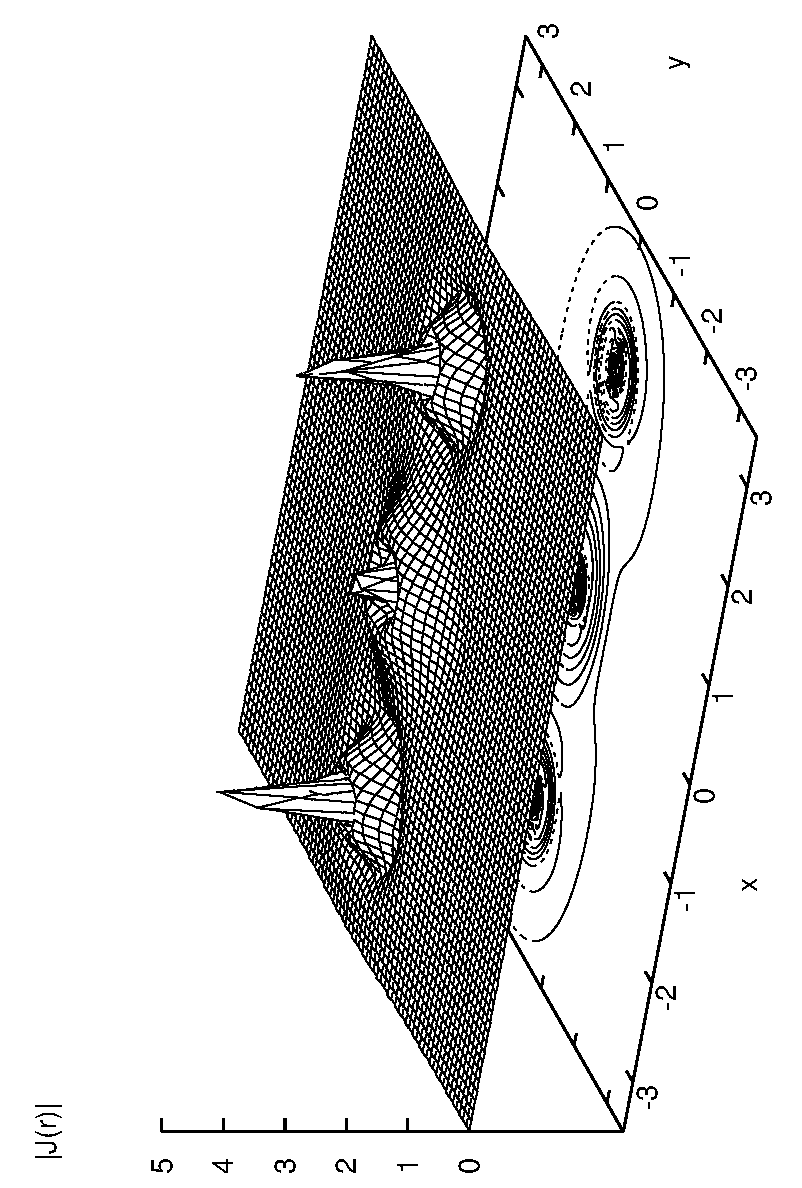
\includegraphics[clip=0,scale=0.33,angle=-90]{co2_modsurf}}
\subfigure[]{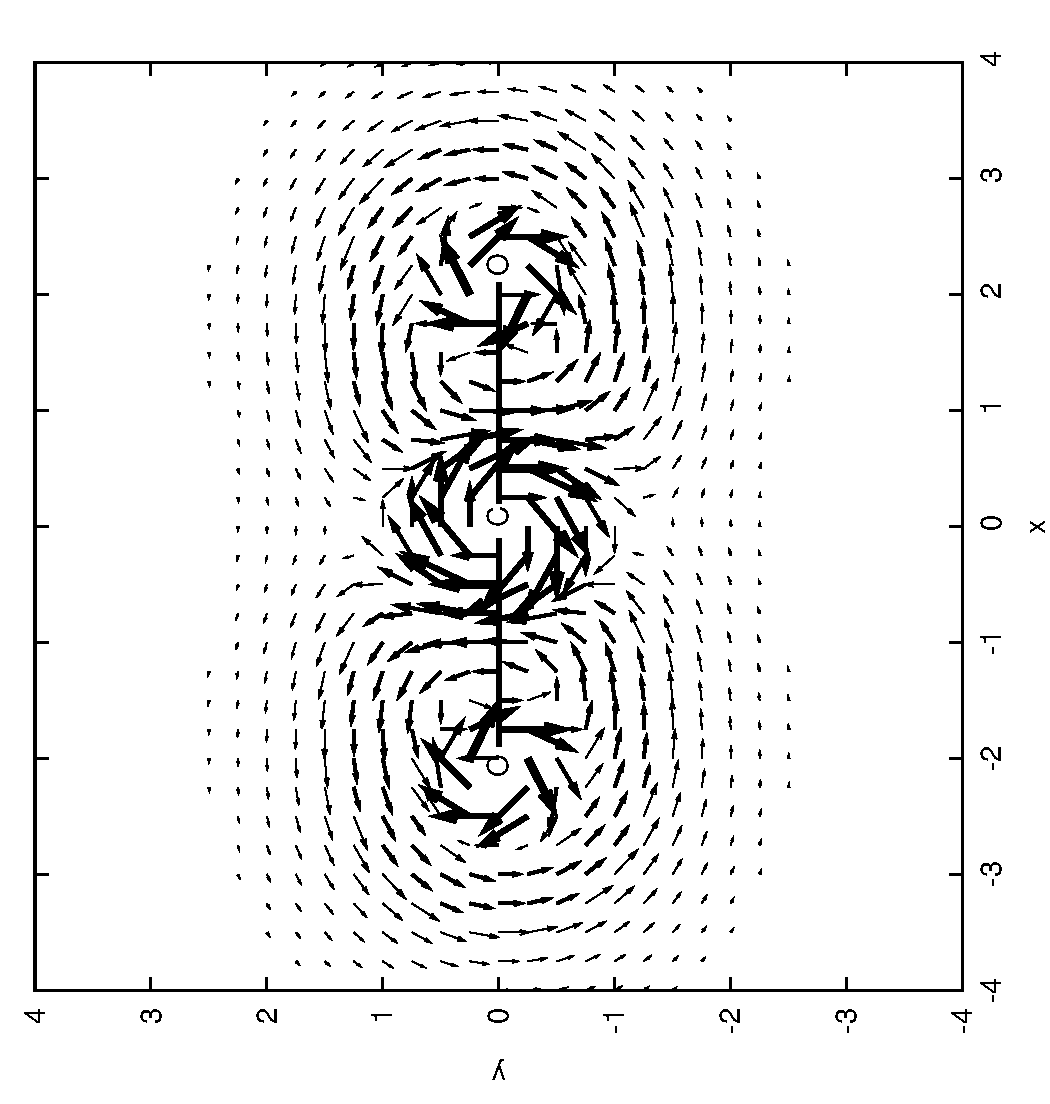
\includegraphics[clip=0,scale=0.33,angle=-90]{co2_jvec}}
\caption{The magnitude (a) and direction (b) of the induced current
density (in au) calculated in the molecular plane of CO$_2$ at 
the CCSDT/TZP level.}
\label{co2_fig}
\end{center}
\end{figure}

\subsection{Integration of current densities}
\label{sec:int}
Although the current density is a proper quantum mechanical observable, it has
not been directly observed experimentally. As such, current-density maps can
convey new, otherwise inaccessible, information about molecules, thus aiding
the understanding of the current paths in the molecule.  However,
current-density plots do not provide any quantifiable measures of the current
strengths nor are they suitable for comparing  current strengths in different
molecular systems.  By integration
over the current flow passing through specific bonds, it is possible to obtain
the net current strengths around a molecular ring or through a bond.  In
non-cyclic molecules, the net current flow must be zero, in order
for the law of charge conservation to hold. 

Integration of the current density is done using 
two-dimensional Gaussian or Lobatto quadrature \cite{Abramowitz:65} over a
bond cross section (see \Fig{bondcross}).  
The Gauss integration points $x_i$ are given by the nodes
of the Legendre polynomials $P_n(x)$, while the integration weights $w_i^{G}$
are obtained from the differentiated polynomials,
$\left(\frac{dP_n(x_i)}{dx}\right)$.  In one dimension, Gauss quadrature
yields 
\begin{equation}
\int_{a}^{b} f(x)dx=
\sum_{k=1}^{m} \left(\sum_{i=1}^{n}w_i^{G}f_{k}(x_i)\right),
\end{equation}
where the sum over $k$ originates from the piecewise integration and $f_k$ is
the function $f$ shifted to $[-1,1]$ on the $k$th interval.  The integration
weights are given by
\begin{equation}
w_i^{G}=\frac{2}{1-x_i^2}\left(\frac{dP_n(x_i)}{dx}\right)^2.
\end{equation}

\begin{figure}
\begin{center}
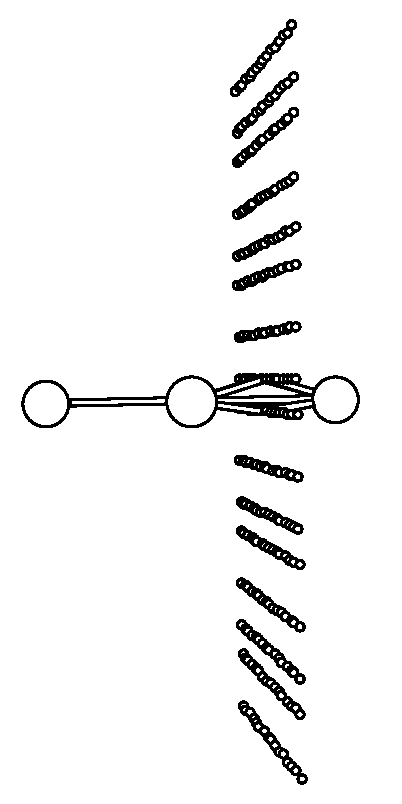
\includegraphics[clip=0,scale=0.25,angle=0]{bond_int}
\caption{A typical integration grid through a bond.}
\label{bondcross}
\end{center}
\end{figure}
In the Lobatto integration, the integration points are determined via the
nodes of the first derivative of the Legendre polynomials of order $n-1$,
$\left(\frac{dP_{n-1}(x)}{dx}\right)$.  In addition, the function values at
the end points of the interval are also considered in the Lobatto integration.
The integration weights $w_i^{L}$ are obtained from  $P_{n-1}(x_i)$. The
one-dimensional Lobatto quadrature then reads
\begin{equation}
\int_{a}^{b} f(x)dx=
\sum_{k=1}^m\left(w_1^{L}f_{k}(-1)+w_n^{L}f_{k}(1)+
\sum_{i=2}^{n-1}w_i^{L}f_{k}(x_i)\right),
\label{lobwgt}
\end{equation}
with the corresponding weights given by
\begin{equation}
w_i^{L}=\frac{2}{n(n-1)\left(P_{n-1}(x_i)\right)^2},
\end{equation}
and the integration weights for the end points by
\begin{equation}
w_1^{L}=w_n^{L}=\frac{2}{n(n-1)}.
\end{equation}
Numerical values for the integration points and weights are tabulated in
Ref.~\cite{Abramowitz:65}. Alternatively they can be obtained by solving 
the roots to the derivative of the Legendre polynomials, using for example
Newton's method.

Cyclic systems such as aromatic molecules can sustain a net current that flows
around the molecular rings. The net current should in principle be independent 
of where in the ring it is calculated. Due to practical issues, this is not
necessarily always the case. In the numerical integration of the currents
passing a given bond, one has to be careful where and how to cut the bond.
The choice of grid and method of integration is, by far, less critical.  For
benzene, a fairly good convergence of the integrated current is achieved with
a grid that starts in the ring center, passes through the center of the bond,
and is perpendicular to the molecular plane. The integration area has to be
extended to about 5 Bohr outside the bond and 5 Bohr above and below the ring.
Then, it incorporates the most significant part of the current flow.  In
principle, it does not matter for which bond cross section the ring current is
integrated, but it is recommended to use cross sections containing the bond
midpoint. The reason is that due to the poles at the nuclei the 
current-density vector field can be rather strong in the vicinity,
which thus renders integration more difficult. 
Dense grids are then needed to converge the integrals, while,
for integrations over bond cross sections containing the bond midpoint, as few
as 20 grid points in each direction are often sufficient for obtaining
accurate integral values. The divergence problem discussed in the next
subsection also suggests that the integration plane is chosen as far away from
the nuclei as possible.

For non-cyclic molecules (e.g. carbon dioxide, ozone) the net current is 
necessarily zero. In spite of this, it is still possible to obtain the
strength  of the current in individual bonds by splitting the integral into 
positive and negative contributions, or alternatively, by integrating over only 
half of the bond cross section. Currents obtained in such a way are however
dependent on the location of the cut-plane. Such ''bond currents'' might prove
useful as a measure of electron delocalization.

\subsection{Current conservation in the GIMIC method}
As mentioned earlier, the current obeys the law of charge conservation, {\it
i.e.}~the divergence of the current, $\nabla\cdot\mbf{J}$, must be zero at
{\em every} point of
space\footnote{This requirement holds for time-independent systems. For
time-dependent systems, the divergence must be equal to a corresponding change
of the density at time $t$.}.  Alternatively, the law of charge conservation
can be expressed using the Sambe-Epstein integral condition for charge-current
conservation \cite{Lazzeretti:00}  
\begin{equation}
\int \mbf{J(r)}\cdot d{\bf r} = 0.
\end{equation}
For molecules with a center of inversion this integral is for 
symmetry reasons equal to zero, whereas for molecules of low symmetry, 
\Eq{SambeEpstein} is fulfilled only when charge is conserved. Requiring the 
divergence to be zero is thus a better criterion, 
as it is a local measure of charge conservation.

The law of charge conservation can also be viewed as a consequence of gauge
invariance \cite{Epstein:73}. Thus, if true gauge invariance is not achieved,
the calculated current will to some extent be divergent. Epstein has shown
that the use of GIAOs does not necessarily lead to the desired current
conservation \cite{Epstein:73} even though the magnetic shielding tensor is
gauge-origin independent. This is not surprising, since the GIAO approach can
be viewed as a recipe for the unique definition of a set of local
gauge-origins for the basis functions.  Gauge-origin dependence is in this way
eliminated, but gauge invariance cannot achieved in this manner.

By calculating the divergence of the current ($\nabla\cdot\mbf J(\mbf r)$) in
selected points of space, one can obtain a measure of the gauge-independence 
errors, and thus of the basis-set completeness. In our work, the divergence is
calculated by using numerical differentiation on a locally tight grid. 

Calculations of the divergence for H$_2$ and CO$_2$ at the HF-SCF
level showed that the divergence of the current significantly deviates
from zero in the vicinity of the nuclei, and in regions where the direction of
the current changes rapidly. By systematically augmenting the basis sets 
with functions of higher $l$-quantum numbers,
the divergence converges towards small values even close to
the nuclei [see Figure~\ref{divj_fig}(b) and (c)]. 
For H$_2$, the use of a basis set of cc-pV5Z quality to 
reduces the maximum value of the  divergence to a value
which is for all practical purposes equal to zero. The same quality basis for
CO$_2$ still yields non-zero divergence near the nuclei. Discouraging as
this may seem, a corresponding HF-SCF/SVP calculation without GIAOs  
and with the gauge origin at the carbon atom yields a maximum
value of the divergence which is more than factor of fifteen 
times larger than the largest divergence of the GIAO calculation. 
In the conventional calculation, the divergence also has
a much broader spatial distribution. The effect of the GIAOs on
the divergence can clearly be seen in Figure~\ref{divj_fig} (a) and (b).

\begin{figure}
\begin{center}
\subfigure[]{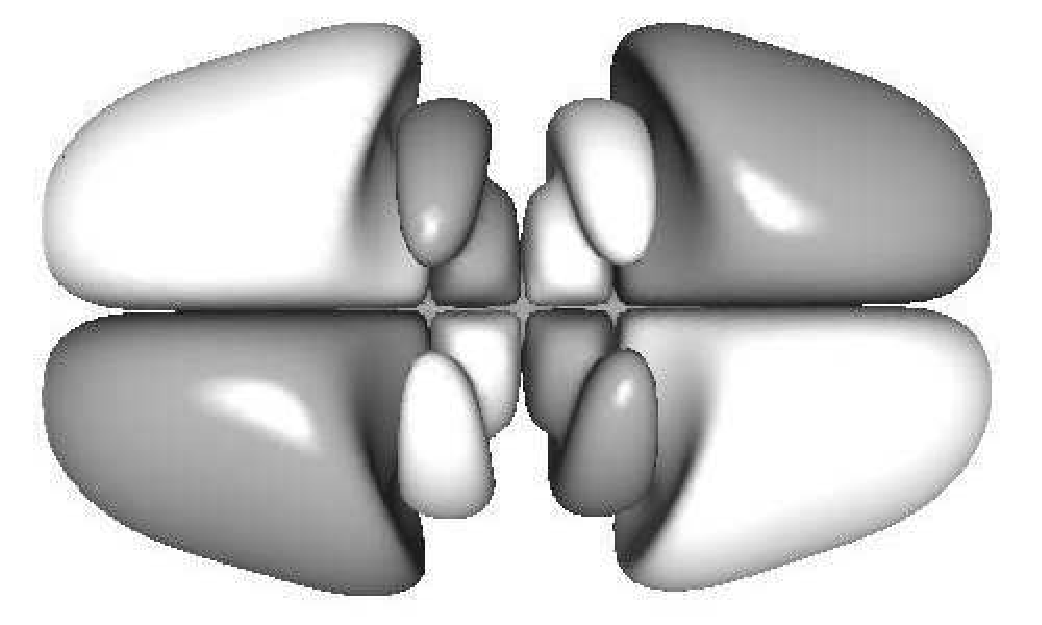
\includegraphics[clip=0,scale=0.23]{divj_svp_conv}}
\subfigure[]{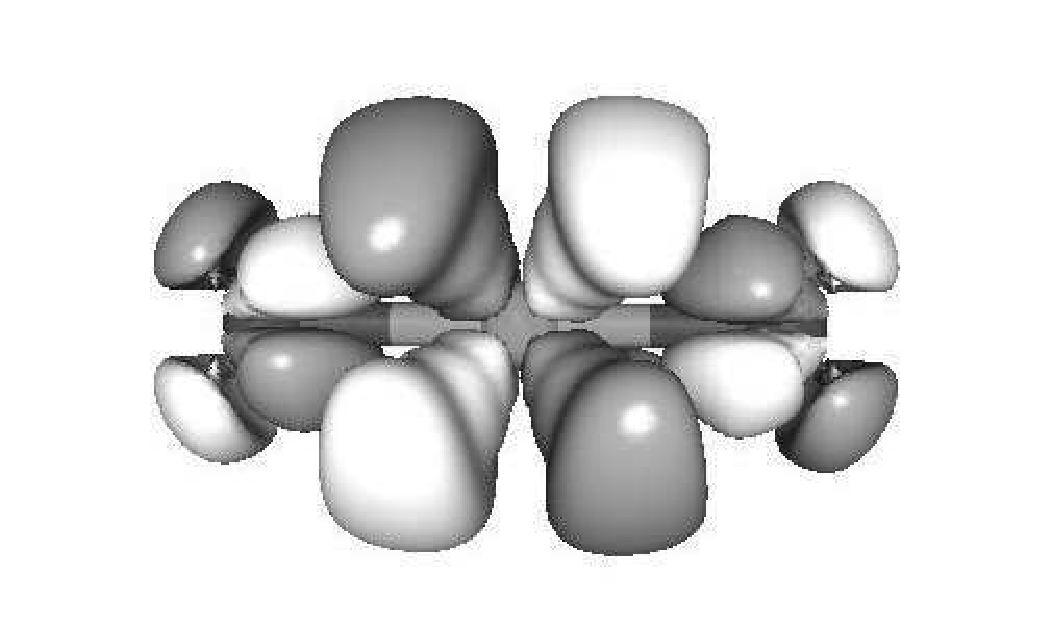
\includegraphics[clip=0,scale=0.23]{divj_svp}}
\subfigure[]{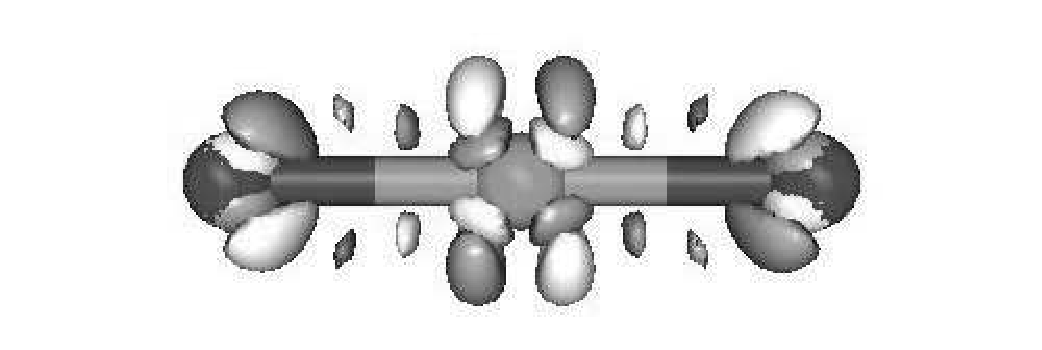
\includegraphics[clip=0,scale=0.23]{divj_pv5z}}
\caption{The divergence of the current in CO$_2$ obtained in 
a conventional HF-SCF/SVP calculation (a). The corresponding 
divergence plots obtained at the GIAO HF-SCF/SVP 
and the GIAO HF-SCF/cc-pV5Z levels are depicted in (b) and (c),
respectively.  The iso-surfaces
have been drawn to encompass any divergence larger than 0.01.}
\label{divj_fig}
\end{center}
\end{figure}

Judging whether a divergence is large or not always easy. 
Therefore, one has to examine other properties of the current to be 
able to evaluate the quality of the results. 
The difference in the currents calculated at the HF-SCF/SVP and HF-SCF/cc-pV5Z
levels is found to be small. 
%(see Figures~\ref{co2_fig},
%\ref{diff_divj_fig}. 
%\begin{figure}[H]
%\begin{center}
%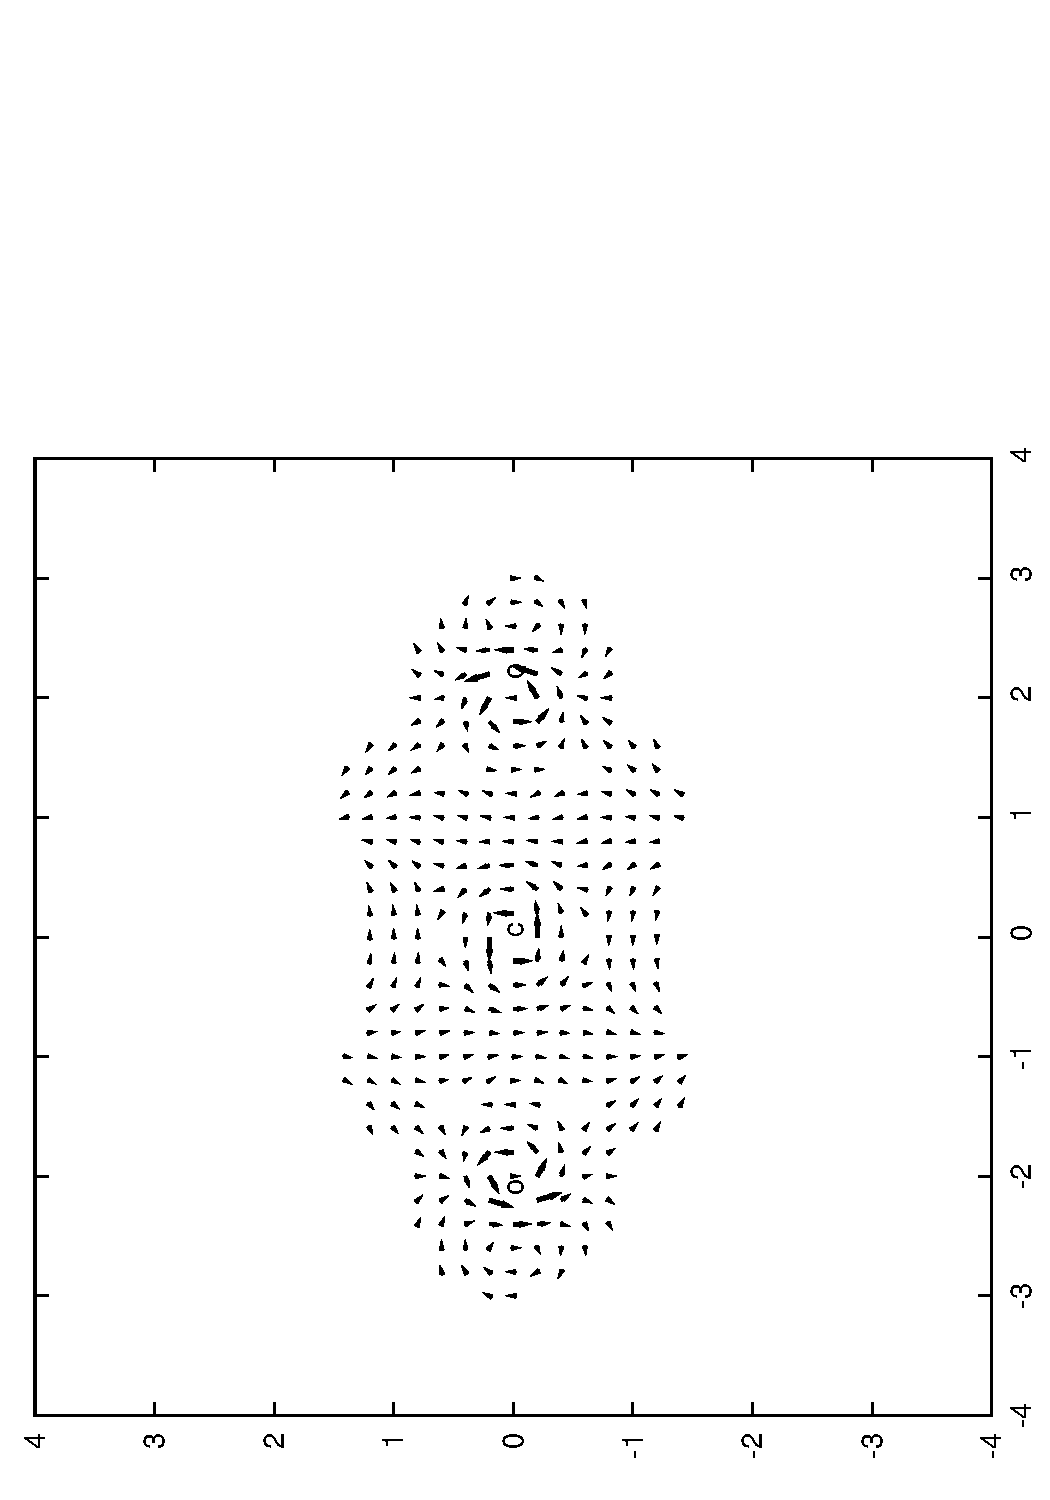
\includegraphics[clip=0,scale=0.25, angle=-90]{co2_diff_divj1.ps}
%
%\caption{The difference between induced current in CO$_2$ obtained 
%using the SVP and cc-pV5Z basis sets.}
%\label{diff_divj_fig}
%\end{center}
%\end{figure}

By studying the
convergence of the integrated current through a bond, one finds that the induced
current only changes by few percent when increasing the basis-set size from
SVP to cc-pV5Z. At the HF-SCF level, the integrated value for the current
passing half of the bond in CO$_2$ decreases from 10.03 to 9.81~nAT$^{-1}$ when
increasing the basis-set size from SVP to cc-pV5Z. For non-cyclic molecules,
for which the symmetry does not constrain the total current to
be zero, the effects of the non-zero divergence can be seen more clearly.
In water and ozone, which belong to the  C$_{2v}$ point group,  
the integrated current through the symmetry plane is particularly hard 
to converge to zero, because the cut plane goes through a 
nucleus where the divergence is large. For water, the difference between
positive and negative current contributions calculated at the HF-SCF/SVP level
is 0.68 nAT$^{-1}$ as compared to the individual contributions of 
24.67 nAT$^{-1}$ and -23.99 nAT$^{-1}$, 
respectively. The corresponding values obtained in a HF-SCF/cc-pV5Z calculation 
are 0.0002 nAT$^{-1}$, 23.4171 nAT$^{-1}$ and -23.4169 nAT$^{-1}$, 
respectively.
By evaluating the Sambe-Epstein condition in Eq.~(\ref{SambeEpstein})
separately for each tensor component, one can estimate the
total current leakage. At the HF-SCF/SVP level, the total leakage 
of the $xy$ and $yx$ components of the current tensor is -3.95 
and 2.45 nAT$^{-1}$ for water, respectively, whereas at the HF-SCF/cc-pV5Z
level, the corresponding values are -0.2295 nAT$^{-1}$ and 0.0044 nAT$^{-1}$.
Thus, even though the divergence is not equal to zero in every point in space
and the current leakage does not seem to be negligible, the integrated
currents are pretty well converged even when using fairly small standard basis
sets. 

\begin{figure}[!hb]
\begin{center}
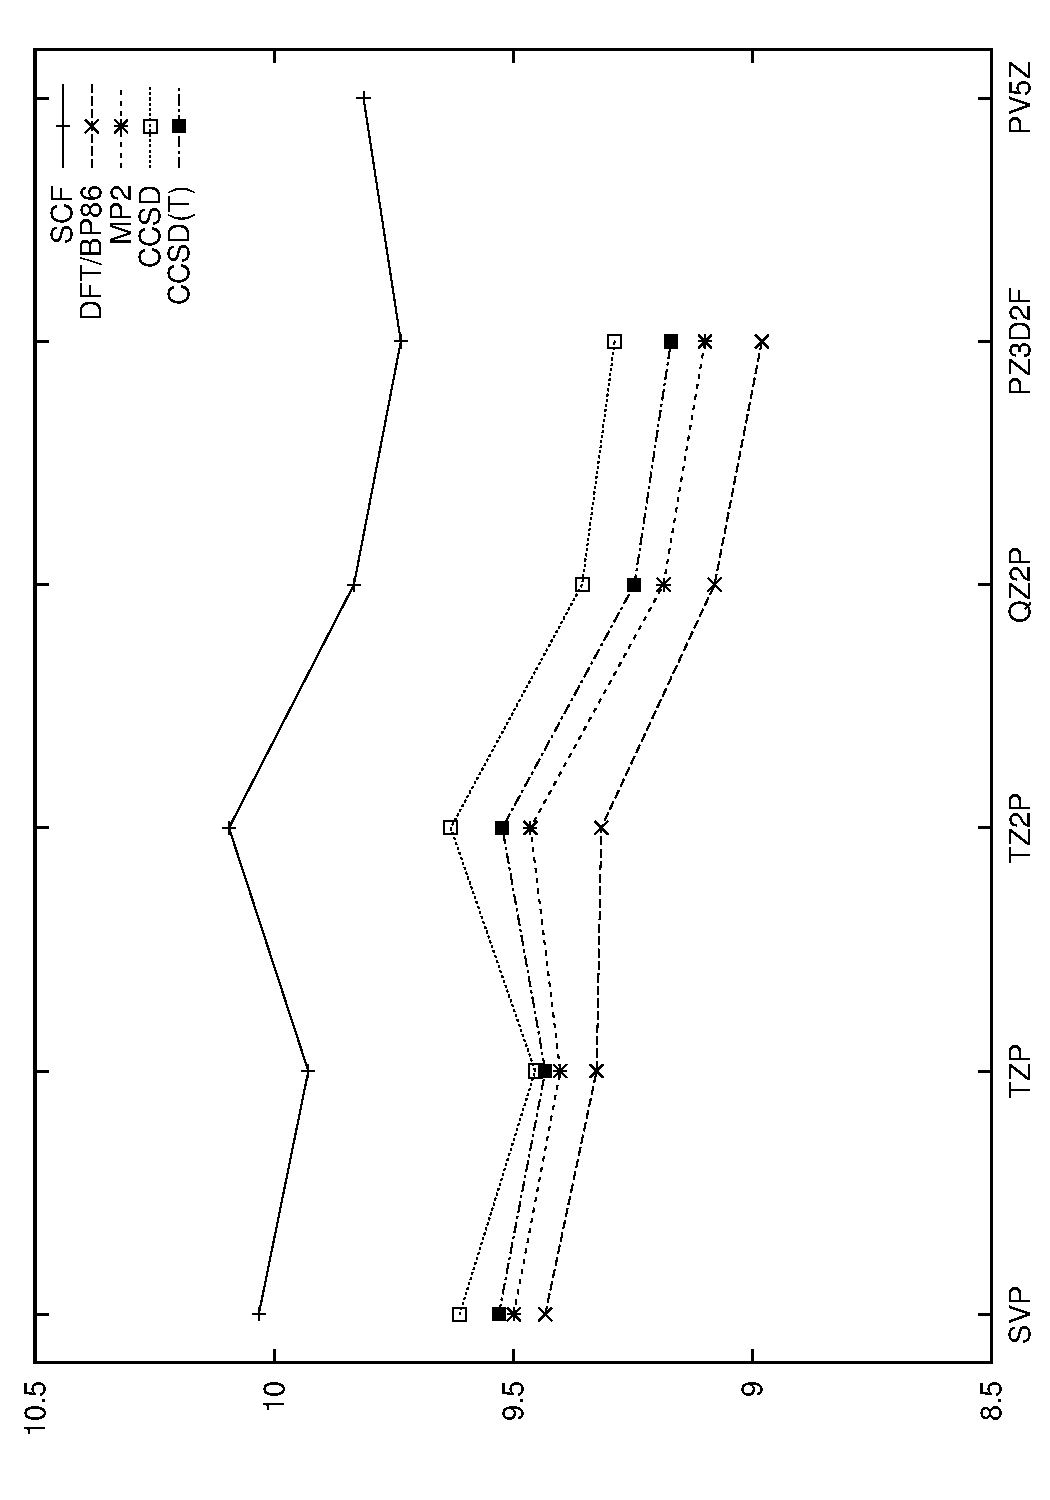
\includegraphics[clip=0,scale=0.3,angle=-90]{co2_bconv}
\caption{The basis-set convergence for the induced current (in nAT$^{-1}$)
calculated at the HF-SCF, DFT-BP86, MP2, CCSD, and CCSD(T) levels for CO$_2$.
}

\label{co2_bset}
\end{center}
\end{figure}
\chapter{Summary and outlook}
\label{ch:synopsis}
When the work upon which this thesis is based was started, we were
interested in the aromaticity and the aromatic pathways of free-base 
porphyrins. We set out trying to analyze the aromaticity using the, then
new, NICS method. Quite soon we found ourselves head deep in data which proved
very hard to draw any final conclusions from. Instead of drawing far-fetched 
conclusions, we started experimenting with the NICS approach, adding NICS
points in the direction perpendicular to the molecular plane. 
This experimenting lead to the ARCS method which is
presented in \citetalias{Juselius:t99}. In this paper we developed the ARCS
analysis and applied it to a number of simple aromatic and non-aromatic
molecules. 

At this stage, we were confident that we had a much more reliable
method than the original NICS method. In \citetalias{Juselius:t00} 
we returned to the porphyrin
problem, and using the ARCS method we analyzed the aromaticity and the current
pathways. To resolve the current pathways in these fused-ring 
systems, we saturated certain bonds, effectively preventing any current to take
that route. By calculating the current strengths, we were able to deduce the
preferred paths indirectly.  In the original ARCS paper, we had also tried to
use a 2D-NICS, in which two-dimensional layers of NICS points were calculated
at some distance from the molecular plane. This approach, which we called
Planar ARCS (PARCS), came in handy for giving additional evidence for our
conclusions. It is interesting to note that our conclusions about free-base
porphyrin, were later verified using the GIMIC method \cite{Juselius:t04}. In 
\citetalias{Juselius:t00a} we studied the aromaticity of magnesium porphyrins.
In this paper, we asked the question, of the significance of the inner
hydrogen pair 
for the ring current. This paper was in a sense an extension of the previous
paper.  In retrospect it is maybe not very surprising that the effect of the
inner hydrogens was quite small. This could be anticipated, as the ring
current was not much affected by the position of the inner hydrogens in most
cases.

Having studied a number of aromatic systems, next we turned our interest to
some antiaromatic and potentially antiaromatic molecules. In
\citetalias{Juselius:t01} we
studied the ring-current strengths of dehydro[12]annulenes and
dehydro[18]annulenes, which are the building blocks of some new carbon
allotropes which have been proposed \cite{Haley:97,Eickmeier:97,Wan:00,
Diederich:92}. We found that the unsubstituted
dehydro[12]annulene indeed was antiaromatic, but also, that when fused with
benzene or cyclobutadiene rings, the antiaromaticity was destroyed in favor of
aromaticity of the fused rings. Dehydro[18]annulene was found to be diatropic,
but like dehydro[12]annulene, the overall ring current was destroyed upon fusion
with benzene or cyclobutadiene. These findings make it unlikely that graphyne
or graphdiyne, if ever synthezised, will have any particularly exalted
magnetic properties.

In 2001, Wang {\em et al.} synthesized a new and exciting group of molecules,
containing small four membered aluminum rings \cite{Li:01}. 
The general structure of these
molecules is Al$_4^{-}$M where M=Li$^+$, Na$^+$ or Cu$^+$. Based on
photo-electron spectra and calculations, they concluded that these molecules
had significant aromatic character. In \citetalias{Juselius:t01a}, 
we used the ARCS method to
study the ring-current strengths of Al$_4^{2-}$, and also the group III
analogues Ga$_4^{2-}$, In$_4^{2-}$ and Tl$_4^{2-}$, and found that they are
indeed aromatic. Furthermore, we also proposed a number of new, and neutral,
Al$_4^{2-}$ analogues, Si$_2$B$_2$, Si$_2$Al$_2$ and Si$_2$Ga$_2$ all of which
should be aromatic.  In a forthcoming paper \cite{Juselius:t04} we have studied
a number of Al$_4^{2-}$ and Al$_4^{4-}$ species using the GIMIC method, and
found that the diamagnetic part of the ring-current comes from the
$\sigma$-electrons. In Al$_4^{2-}$ the $\pi$-electrons also contribute to the
diamagnetic current, making the magnetic response diamagnetic overall. In
Al$_4^{4-}$, however, the $\pi$-electrons give rise to a paramagnetic current,
effectively canceling the total current. Still, Al$_4^{4-}$ seem to
sustain {\em both} a diatropic and a paratropic current in the same system!

The last class of molecules we studied primarily using the ARCS method, was a
group of potentially homoaromatic molecules of the general form
C$_n$H$_{n+1}^x$, with n=4-13 and x=-1,0,+1,+2. These molecules 
are significantly non-planar since the conjugated ring is interrupted
by single bonds. The concept of homoaromaticity has been much debated, and
in \citetalias{Juselius:t03} we were able to show that of the studied
molecules, C$_8$H$_9^+$ (homotropylium cation), C$_9$H$_{10}^{2+}$,
C$_{10}$H$_{11}^-$ and C$_{12}$H$_{13}^+$ can sustain strong ring currents. 
\citetalias{Juselius:t03} also shows some spectacular shortcomings of the NICS
method.

The articles discussed so far form a logical whole. Starting from the
methodological paper, which included calculations on some simple test systems,
in the following papers we apply the method to a variety of systems of much
more demanding character, covering most aspects of aromaticity. Although the
ARCS method has proven to be very useful and quite reliable, it also became
evident that it has a number of limitations. During the work done on porphyrins,
it became evident that resolving the ring-current pathways is far from trivial
using the ARCS method. Some of the aluminum rings posed their own problems,
when the aromatic ring was hindered by counter-ions, making the ARCS analysis
tricky. Finally the work on homoaromatic molecules drew our attention to the
problems of non-planar molecules. In these molecules, it is not {\em a priori}
clear how to define an origin for the ARCS points nor the direction which is
perpendicular to the ring.

These shortcomings lead to the conclusion that what was needed was an explicit
method to calculate the induced current in molecules. Instead of calculating
the current indirectly, direct integration of the current through a dividing
surface gives a precise measure of the net current in aromatic molecules. 
\citetalias{Juselius:t04} discusses the explicit calculation of magnetically
induced currents, presenting the GIMIC method in detail. 
In the GIMIC paper, we showed how to calculate the
current in terms of derivative theory. Using a density matrix formalism, we
were able to calculate currents at various levels of theory. The need for
correlated wave functions arises when studying difficult species like the
Al$_4$ rings, which require an accurate CCSD wave function to give good
results.

The work presented in this thesis is the result of many fruitful
collaborations. My own contribution to
the methods presented in this thesis has been substantial. When we developed
the ARCS method (Articles I and II), 
I was intimately involved in both developing the ideas for
the method as well as in the writing process of the article that resulted. I
also single-handedly wrote all the software needed to do the ARCS and PARCS
analysis. I was also very much involved in the work, that led to the three 
papers on porphyrins, magnesium porphyrins and dehydroannulenes (Articles
II-IV). My input involved ideas on how to resolve the structure of the
current, doing the actual calculations and also partially writing the
articles. My contribution to the papers on Al$_4^{2-}$ and homoaromatic
molecules (Articles V and VI) is more technical, doing part of the
calculations and all of the ARCS calculations, and I do not want to claim much
credit for the original ideas presented in the papers. Finally, already while
working on the ARCS method, I realized the need for a method capable of
explicitly calculating the induced current density and integrating the
current, on order to obtain a better aromaticity index. The ideas of how this
could be done, were born in a collaboration with Dage Sundholm and J�rgen
Gauss. During my first visit to Mainz I derived the necessary theory needed
for a computer implementation. Subsequently I implemented the theory in the
computer program {\sc Gimic}, which has been used for all explicit current
calculations presented in this thesis. The paper on the GIMIC method (Article
VII), is to a large extent written by myself.

\newpage
\renewcommand\bibname{References}
\addcontentsline{toc}{chapter}{\bibname}
\bibliography{thesis}

%\addcontentsline{toc}{chapter}{\indexname}
%\printindex

%\chapter*{Appendix}
%\addcontentsline{toc}{chapter}{Appendix}

\ifappendix
\newcommand{\myart}[1]{%
\ifcase#1
Juselius:t99\or 
Juselius:t00\or
Juselius:t00a\or 
Juselius:t01\or
Juselius:t01a\or
Juselius:t03\or 
Juselius:t04\or 
Juselius:t04c\fi
}%

\newpage
\newcounter{foo}
\setcounter{foo}{0}

\pagestyle{empty}
\whiledo{\value{foo}<7}{
%    \addcontentsline{toc}{chapter}{\citetalias{\myart\thefoo}}
%    \vspace*{6cm}
%    {\hfill\huge\bf \citetalias{\myart\thefoo}}
%    \vspace{1.5cm}
	
	\chapter*{\vspace*{5cm}\centerline{\citetalias{\myart\thefoo}}}
	\thispagestyle{empty}

	\begin{centering}
	{\large\bibentry{\myart\thefoo}.}
	\end{centering}
	\vfill\eject\newpage
	\ifpdf
	\phantom,
	\vfill\eject\newpage
%    \includepdf[pages=-]{Article\thefoo.pdf}
	\fi

	\addtocounter{foo}{1}
}
\fi


\end{document}

